\documentclass{bts-report-ar}

%% ============================================================
%% إعدادات الميتاداتا ومعلومات المذكرة
%% ============================================================
\themeAr{تصميم وإنجاز تطبيق ويب لتسيير ومعايرة معدات القياس والمترولوجيا الصناعية}
\themeFr{Conception et R\'ealisation d'une Application Web de Gestion de la Calibration des \'Equipements de Mesure et de M\'etrologie Industrielle}
\hostorg{المخبر الوطني للمعايرة والمترولوجيا الصناعية (LNEMI)}
\supervisor{الأستاذة بن عياش سميرة}
\promoter{السيد سمير محالبي}
\students{خنشالي محمد باسيم (Khanchali Mohamed Bassem)}
\promotion{2024 / 2026}

\begin{document}
\setRTL

%% ============================================================
%% صفحة الغلاف الرسمية
%% ============================================================
\maketitlepage

%% ============================================================
%% الصفحات التمهيدية (ترقيم روماني)
%% ============================================================
\pagenumbering{roman}
\setcounter{page}{1}

%% ------------------------------------------------------------
%% شكر وعرفان
%% ------------------------------------------------------------
\begin{shokr}
أود أن أتقدم أولاً بالشكر الجزيل لله سبحانه وتعالى على ما أنعم به علينا من توفيق وصحة وعزيمة لإتمام هذا العمل المتواضع والوصول إلى نهاية هذا المسار التكويني الواعد.

كما أعبر عن عميق امتناني وتقديري للأستاذة المشرفة \textbf{بن عياش سميرة} على دعمها المستمر وتوجيهاتها القيمة ونصائحها السديدة طوال فترة إنجاز هذا المشروع.

وأخص بالشكر المؤطر في المؤسسة المستقبلة \textbf{السيد سمير محالبي} على جهوده القيمة، وتعاونه البناء، وحرصه الدائم على تزويدنا بكل ما يفيد لإنجاح هذا العمل وربطه بالمعايير الصناعية المعتمدة.

كما أتوجه بالشكر والتقدير إلى السادة أعضاء لجنة المناقشة والتحكيم لتفضلهم بقبول تقييم هذه المذكرة، وإلى كافة الأساتذة وأعضاء هيئة التدريس والإدارة في \textbf{المعهد الوطني المتخصص في التكوين المهني (INSFP) رحمانية - سيدي عبد الله}، على ما بذلوه من جهد لتوفير أفضل الظروف لتكويننا طيلة فترة دراستنا.

وأخيراً، أتقدم بالشكر إلى جميع الزملاء والأصدقاء وكل من ساهم من قريب أو من بعيد في إنجاز هذا المشروع.
\end{shokr}

%% ------------------------------------------------------------
%% إهداء
%% ------------------------------------------------------------
\begin{ihda}
\begin{center}
\vspace*{2cm}
{\itshape
أهدي هذا العمل المتواضع :

إلى الينبوع الذي لا ينضب من الحنان والعطاء، إلى من رعتني بصبرها ودعواتها المباركة، إلى أغلى ما أملك في الوجود : \textbf{أمي الغالية}.

إلى من علمني الكفاح وعزة النفس وغرس في نفسي حب العلم والعمل، إلى قدوتي ومثلي الأعلى، إلى من غاب عن عيني وبقيت ذكراه حية في قلبي : \textbf{روحي والدي الطاهرة} (رحمه الله وأسكنه فسيح جناته).

إلى إخوتي وأخواتي الأعزاء، على مساندتهم الدائمة وتشجيعهم المستمر لي في كافة مراحل دراستي.

إلى عائلتي الكريمة وأقاربي على دعمهم المعنوي.

إلى كل أصدقائي وزملائي في الدراسة الذين تقاسمت معهم أجمل اللحظات.

إلى كل من يسعى في طلب العلم وخدمة المجتمع.
}
\end{center}
\end{ihda}

%% ------------------------------------------------------------
%% الملخصات (عربي، فرنسي، إنجليزي)
%% ------------------------------------------------------------
\begin{abstractar}
تعتبر المترولوجيا الصناعية والمعايرة الدورية لمعدات وأدوات القياس من الركائز الاستراتيجية الأساسية لضمان جودة المنتجات، ودقة التصنيع، وتحقيق مطابقة المعايير الدولية (ISO/IEC 17025). 

يقدم هذا العمل تصميم وإنجاز تطبيق ويب متكامل ومخصص لتسيير دورة الحياة الشاملة لعمليات معايرة وتدقيق الأجهزة القياسية عبر ستة مجالات فيزيائية رئيسية (الضغط، الحرارة، الكهرباء، الأبعاد، الوزن والكتلة، وعزم الدوران). تسمح هذه المنصة بالربط الفعال والمباشر بين الزبائن من المؤسسات الصناعية، المصلحة التجارية، مسؤولي مخبر المترولوجيا، والتقنيين المؤهلين لتنفيذ التجارب. 

تم تطوير النظام وفق معمارية برمجية حديثة تعتمد على إطار العمل \textbf{Laravel 12} مع تقنية \textbf{Inertia.js} ومكتبة \textbf{React 19} ولغة \textbf{TypeScript}، وقاعدة بيانات \textbf{MySQL}، مع إدماج نظام صلاحيات محكم (RBAC)، وعزل كامل لبيانات الزبائن، وضمان عدم قابلية تعديل شهادات المعايرة النهائية، ومتابعة آلية لصلاحية العتاد المرجعي، وسجل تدقيق أمني شامل لكافة العمليات. تم تأكيد موثوقية التطبيق من خلال 67 اختباراً مؤتمتاً بنجاح تام.

\vspace{0.6cm}
\noindent\textbf{الكلمات المفتاحية :} معايرة المعدات، مترولوجيا صناعية، Laravel، React، Inertia.js، شهادات المعايرة، الأمان الرقمي، تدقيق العمليات.
\end{abstractar}

\begin{abstractfr}
La m\'etrologie industrielle et l'\'etalonnage p\'eriodique des \'equipements de mesure constituent un pilier strat\'egique incontournable pour garantir la conformit\'e aux normes de qualit\'e internationales (ISO/IEC 17025). Ce m\'emoire pr\'esente la conception et la r\'ealisation d'une application web d'entreprise d\'edi\'ee \`a la gestion int\'egrale du cycle de vie des op\'erations de calibration couvrant six domaines physiques (pression, temp\'erature, \'electricit\'e, dimensionnel, pesage et couple). D\'evelopp\'ee avec Laravel, Inertia.js, React 19, TypeScript et MySQL, la plateforme int\`egre un contr\^ole d'acc\`es RBAC, l'immutabilit\'e des certificats d\'efinitifs, le suivi des \'etalons de r\'ef\'erence et une piste d'audit inalt\'erable. Une suite de 67 tests automatis\'es valide la fiabilit\'e du syst\`eme \`a 100\%.

\vspace{0.6cm}
\noindent\textbf{Mots-cl\'es :} Calibration d'\'equipements, M\'etrologie industrielle, Laravel, Inertia.js, React, Certificats officiels, Immutabilit\'e, Piste d'audit.
\end{abstractfr}

\begin{abstracten}
Industrial metrology and periodic equipment calibration represent a vital foundation for ensuring precision manufacturing, operational safety, and compliance with international quality standards such as ISO/IEC 17025. This thesis presents the comprehensive design and engineering of an enterprise web platform managing the end-to-end lifecycle of measurement equipment calibration across six physical domains (pressure, temperature, electrical, dimensional, mass, and torque). Built with Laravel, Inertia.js, React 19, TypeScript, and MySQL, the platform enforces role-based authorization (RBAC), multi-tenant client isolation, strict immutability of finalized calibration certificates, automated reference standards expiration alerts, and comprehensive audit trail logging verified by 67 automated tests.

\vspace{0.6cm}
\noindent\textbf{Keywords :} Equipment Calibration, Industrial Metrology, Laravel, Inertia.js, React, Digital Certificates, Immutability, Audit Trail.
\end{abstracten}

%% ------------------------------------------------------------
%% فهارس المحتويات والأشكال والجداول
%% ------------------------------------------------------------
\tableofcontents
\listoffigures
\listoftables

%% ------------------------------------------------------------
%% قائمة الاختصارات
%% ------------------------------------------------------------
\chapter*{قائمة الاختصارات (Glossaire)}
\addcontentsline{toc}{chapter}{قائمة الاختصارات}

\begin{abbrevtablear}
  \ucfieldar{BTS}{شهادة تقني سامي (Brevet de Technicien Supérieur)}
  \ucfieldar{INSFP}{المعهد الوطني المتخصص في التكوين المهني}
  \ucfieldar{LNEMI}{المخبر الوطني للمعايرة والمترولوجيا الصناعية}
  \ucfieldar{ISO}{المنظمة الدولية للتقييس (International Organization for Standardization)}
  \ucfieldar{IEC}{اللجنة الكهروتقنية الدولية (International Electrotechnical Commission)}
  \ucfieldar{UML}{لغة النمذجة الموحدة (Unified Modeling Language)}
  \ucfieldar{UP}{المنهجية الموحدة للتطوير (Unified Process)}
  \ucfieldar{MVC}{نمط المعمارية البرمجية: نموذج - واجهة - متحكم (Model - View - Controller)}
  \ucfieldar{SPA}{تطبيق الصفحة الواحدة (Single Page Application)}
  \ucfieldar{API}{واجهة برمجة التطبيقات (Application Programming Interface)}
  \ucfieldar{RBAC}{التحكم في الوصول المعتمد على الأدوار (Role-Based Access Control)}
  \ucfieldar{ORM}{رسم الخرائط العلائقية للكائنات (Object-Relational Mapping)}
  \ucfieldar{LEMP}{حزمة خادم الويب: Linux, Nginx, MySQL, PHP}
  \ucfieldar{CSRF}{حماية ضد تزوير الطلبات عبر المواقع (Cross-Site Request Forgery)}
  \ucfieldar{XSS}{حماية ضد البرمجة النصية عبر المواقع (Cross-Site Scripting)}
  \ucfieldar{ACID}{خصائص الموثوقية في قواعد البيانات: الذرية، التناسق، العزل، والديمومة}
  \ucfieldar{HTTP/HTTPS}{بروتوكول نقل النص الفائق الآمن (HyperText Transfer Protocol Secure)}
  \ucfieldar{TLS}{أمان طبقة النقل والتشفير (Transport Layer Security)}
\end{abbrevtablear}


%% ============================================================
%% المتن الرئيسي (ترقيم عربي يبدأ من المقدمة العامة)
%% ============================================================
\pagenumbering{arabic}
\setcounter{page}{1}

%% ============================================================
%% المقدمة العامة
%% ============================================================
\chapter*{المقدمة العامة}
\addcontentsline{toc}{chapter}{المقدمة العامة}

\section*{السياق العام}
في ظل التطور السريع الذي يشهده العالم في مجال تكنولوجيا المعلومات والاتصال، أصبحت الأنظمة الرقمية من أهم الوسائل المعتمدة داخل المؤسسات لتحسين الأداء وتسهيل مختلف العمليات الإدارية والتنظيمية. فقد ساهم التحول الرقمي في تبسيط طرق التسيير، تسريع الوصول إلى المعلومات، وضمان دقة أكبر في معالجة البيانات مقارنة بالطرق التقليدية.

ومع التزايد المستمر في حجم البيانات وتنوع الخدمات داخل المؤسسات الصناعية والخدمية، أصبح من الضروري الاعتماد على حلول معلوماتية حديثة تسمح بتنظيم العمل وتوفير بيئة رقمية فعالة تساعد المستخدمين على أداء مهامهم بسهولة ومرونة.

وتكتسي عمليات المعايرة والمترولوجيا الصناعية أهمية قصوى داخل المنشآت الإنتاجية، حيث أن دقة أدوات القياس (مثل مقاييس الضغط، مجسات الحرارة، أجهزة القياس الكهربائية، وأجهزة الوزن) تحدد بشكل مباشر جودة المنتجات وسلامة المنشآت ومطابقتها للمعايير الدولية الصارمة مثل معيار \textbf{ISO/IEC 17025}. 

وانطلاقًا من هذا الواقع، جاءت فكرة مشروعنا المتمثلة في تصميم وإنجاز تطبيق ويب خاص بـ \textbf{تسيير ومعايرة معدات القياس والمترولوجيا الصناعية}، بهدف تقديم حل رقمي متكامل يساهم في تحسين عملية التسيير، وتتبع مسار المعدات، وإصدار شهادات المعايرة الرسمية بطريقة موثوقة وغير قابلة للتلاعب.

\section*{الإشكالية وفرضية العمل}
رغم التطور التكنولوجي الكبير، إلا أن العديد من مخابر المعايرة والوحدات الصناعية ما تزال تعتمد على طرق تقليدية وشبه يدوية في تسيير بياناتها، مثل السجلات الورقية، وجداول البيانات المنفصلة (Excel)، والمراسلات عبر البريد الإلكتروني العادي. وهو ما يؤدي إلى عدة مشاكل جوهرية:
\begin{itemize}
  \item بطء معالجة الطلبات وطول فترة الانتظار بين تقديم الطلب وإصدار الفواتير التقديرية.
  \item صعوبة التنسيق بين الزبائن والمصلحة التجارية والمسؤولين التقنيين حول مواعيد التدخل.
  \item الخطر المترولوجي المتمثل في احتمال استعمال عتاد مرجعي (Étalons) منتهي الصلاحية دون انتباه المشرفين.
  \item غياب نظام تدقيق أمني يثبت هوية وتاريخ كل تعديل يطرأ على تقارير المعايرة.
  \item بطء تسليم شهادات المعايرة للزبائن مما يعطل عمليات التدقيق والإنتاج لديهم.
\end{itemize}

ومن هذا المنطلق نطرح الإشكالية التالية:
\begin{quote}
\itshape
\og كيف يمكن تصميم وتطوير تطبيق ويب فعال وآمن يساعد على رقمنة وتسيير دورة الحياة الكاملة لعمليات معايرة معدات القياس، مع ضمان سهولة الاستخدام، والسرعة، وعزل بيانات الزبائن، وعدم قابلية تعديل الشهادات النهائية، وتوفير سجل تدقيق أمني شامل لكافة العمليات؟ \fg
\end{quote}

وتقوم فرضية العمل على أن بناء منصة ويب تعتمد على معمارية العميل والخادم الحديثة من خلال دمج إطار العمل \textbf{Laravel 12} مع تقنية \textbf{Inertia.js} ومكتبة \textbf{React 19}، وتطبيق نظام صارم لإدارة الصلاحيات (RBAC)، سيسمح بأتمتة تدفق العمليات، وإلغاء الأخطاء البشرية، وتوفير بيئة موثوقة تحفظ الوثائق القانونية وتضمن تتبعاً تاماً وفق متطلبات الجودة العالمية.

\section*{أهداف المشروع}
يهدف هذا المشروع إلى تحقيق الأهداف الرئيسية التالية:
\begin{enumerate}
  \item رقمنة عملية تسجيل طلبات المعايرة والسماح للزبون بإدخال مجموعة من المعدات المتنوعة في طلب واحد.
  \item تسيير المعالجة التجارية للطلبات من خلال إعداد الفواتير الشكلية (Devis) وتحديد الرسوم القانونية تلقائياً.
  \item إتاحة التنسيق والاتفاق الإلكتروني بين الزبون والمخبر حول تاريخ ومكان المعايرة (في المخبر أو في موقع الزبون).
  \item تنظيم توزيع المهام وجدولة تدخلات التقنيين المترولوجيين ومتابعة مراحل الإنجاز.
  \item المراجعة النوعية للتقارير مع إمكانية طلب تصحيحات تقنية معللة (\textit{Rework}) قبل الاعتماد.
  \item إصدار شهادات معايرة رسمية مؤمنة بنظام يمنع تعديلها أو حذفها نهائياً بمجرد اعتمادها الرسمي (\texttt{is\_final = true}).
  \item تتبع العتاد والأدوات المرجعية للمخبر وتنبيه المشرفين آلياً عند انتهاء صلاحية أي أداة ومنع استخدامها.
  \item توفير سجل تدقيق شامل وغير قابل للإلغاء (\textit{Audit Trail}) يوثق تاريخ واسم صاحب كل عملية وتفاصيل التغييرات.
\end{enumerate}

\section*{خطة المذكرة}
تم تقسيم هذه المذكرة إلى أربعة فصول رئيسية بالإضافة إلى المقدمة العامة والخاتمة العامة، وذلك وفق ما يلي:
\begin{itemize}
  \item \textbf{الفصل الأول: المفاهيم العامة والأسس النظرية :} يتناول المفاهيم الأساسية لشبكة الإنترنت والويب، معمارية العميل والخادم، ونظرة تفصيلية على التقنيات المستعملة في الواجهة الأمامية والخلفية والأمان.
  \item \textbf{الفصل الثاني: الدراسة التمهيدية :} يختص بتقديم المؤسسة المستقبلة (المخبر الوطني للمعايرة)، وهيكلها التنظيمي، ونقد الوضع الحالي، وتحديد المتطلبات الوظيفية والتقنية والمنهجية المتبعة.
  \item \textbf{الفصل الثالث: التحليل والتصميم :} يركز على نمذجة النظام بواسطة لغة UML، من خلال مخططات حالات الاستخدام، والبطاقات الوصفية، ومخططات التسلسل، ومخطط الحالات والانتقالات، ومخطط الفئات وقاموس المعطيات ومخطط النشر.
  \item \textbf{الفصل الرابع: الإنجاز والاختبارات :} يعرض بيئة التطوير، والهيكلة البرمجية، وواجهات التطبيق المنجزة، والنتائج الكاملة لحزمة الاختبارات الآلية المؤكدة لسلامة النظام.
\end{itemize}


%% ============================================================
%% الفصل الأول : المفاهيم العامة والأسس النظرية
%% ============================================================
\chapter{المفاهيم العامة والأسس النظرية}

\section*{مقدمة الفصل}
في ظل التطور التكنولوجي السريع الذي يشهده العالم في السنوات الأخيرة، أصبحت تطبيقات الويب تحتل مكانة أساسية في مختلف المجالات، حيث ساهمت بشكل كبير في تسهيل العمليات اليومية وتحسين أداء المؤسسات والأفراد. فقد أصبحت المواقع والتطبيقات الإلكترونية أداة رئيسية لتقديم الخدمات، تبادل المعلومات، وإدارة مختلف الأنشطة بطريقة أكثر فعالية وسرعة.

ويعتمد نجاح أي تطبيق ويب على مجموعة من المفاهيم والتقنيات الأساسية التي تشكل البنية التحتية لعملية التطوير، بدءًا من شبكة الإنترنت والويب، مرورًا بهندسة العميل والخادم، ووصولًا إلى قواعد البيانات واستضافة المواقع. يهدف هذا الفصل إلى تقديم أهم المفاهيم النظرية المتعلقة بعالم تطوير الويب، والتي تعتبر قاعدة أساسية لفهم مختلف الجوانب التقنية الخاصة بمشروعنا.

\section{تعريف الإنترنت والويب}
\subsection{تعريف الإنترنت}
الإنترنت هي شبكة عالمية ضخمة تربط بين ملايين أجهزة الحاسوب والشبكات حول العالم، وتسمح بتبادل المعلومات والبيانات بين المستخدمين باستخدام حزمة بروتوكولات موحدة أهمها بروتوكول \textbf{TCP/IP}. وتوفر الإنترنت العديد من الخدمات المتنوعة مثل البريد الإلكتروني، ونقل الملفات، والاتصال الصوتي والمرئي، والخدمات السحابية.

\subsection{تعريف الويب}
الويب (\textit{World Wide Web}) هو أحد أهم الخدمات والتطبيقات التي تعمل فوق شبكة الإنترنت، حيث يسمح للمستخدمين بتصفح وثائق ومستندات مترابطة تشعبياً تحتوي على نصوص، وصور، وفيديوهات باستخدام متصفحات الويب الحديثة، والاعتماد على محددات الموارد الموحدة (URL).

\subsection{الفرق بين الإنترنت والويب}
رغم أن الكثير يخلط بين المفهومين في الاستعمال اليومي، إلا أن هناك فرقاً جوهرياً بينهما:
\begin{itemize}
  \item \textbf{الإنترنت :} تمثل البنية التحتية المادية والشبكة العالمية الشاملة التي تربط الأجهزة والخوادم ببعضها.
  \item \textbf{الويب :} هو خدمة ومنظومة برمجية تعمل فوق الإنترنت وتسمح بعرض الصفحات والمواقع وتداول البيانات التفاعلية.
\end{itemize}

\section{أنواع تطبيقات الويب وهندسة العميل والخادم}
\subsection{المواقع الثابتة والديناميكية}
\begin{itemize}
  \item \textbf{المواقع الثابتة (Static Websites) :} تعرض محتوى ثابتاً ومبرمجاً مسبقاً لا يتغير بناءً على تفاعل المستخدم، وتعتمد فقط على لغات العرض مثل HTML و CSS.
  \item \textbf{المواقع والتطبيقات الديناميكية (Dynamic Web Applications) :} تعتمد على خوادم المعالجة وقواعد البيانات لتوليد محتوى مخصص ومتغير في الوقت الفعلي حسب رغبة وهوية المستخدم، وتسمح بإجراء عمليات الحفظ، التعديل، والحساب المعقد، وهو النمط الذي يندرج ضمنه مشروعنا.
\end{itemize}

\subsection{معمارية العميل والخادم ونموذج 3-Tiers}
يقوم النموذج التقليدي لمعمارية العميل والخادم على طرفين أساسيين: \textbf{العميل (Client)} وهو المتصفح أو الجهاز الذي يرسل الطلبات، و\textbf{الخادم (Server)} وهو الجهاز أو التطبيق المركزي الذي يستقبل الطلبات، يعالجها برمجياً، ويرجع النتائج المناسبة.

وقد تم تطوير تطبيقنا بالاعتماد على معمارية الطبقات الثلاث (\textbf{3-Tiers}) التي تضمن تنظيماً محكماً وفصلاً تاماً بين المسؤوليات:
\begin{enumerate}
  \item \textbf{طبقة العرض (Tier 1 - Presentation) :} متصفح الويب لدى المستخدم، ويعتمد على مكونات React 19 ولغة TypeScript لتوفير واجهات تفاعلية وسريعة.
  \item \textbf{طبقة المعالجة والمنطق البرمجي (Tier 2 - Application Server) :} خادم التطبيق المعتمد على إطار العمل Laravel 12، ويتولى فحص المدخلات، وتطبيق الصلاحيات، وإدارة دورة العمليات.
  \item \textbf{طبقة البيانات (Tier 3 - Database) :} نظام إدارة قواعد البيانات MySQL 8.0، المسؤول عن الحفظ الآمن، والالتزام بمعايير المعاملات الموثوقة (ACID).
\end{enumerate}

\begin{figure}[H]
  \centering
  \begin{LTR}
  \resizebox{\textwidth}{!}{\begin{tikzpicture}[>=stealth, node distance=1.5cm and 2cm,
    tier/.style={draw=blue!70!black, fill=blue!5, rounded corners=4pt, line width=1pt, minimum width=3.2cm, minimum height=1.6cm, align=center, font=\small},
    db/.style={draw=orange!80!black, fill=orange!10, rounded corners=4pt, line width=1pt, minimum width=3.2cm, minimum height=1.6cm, align=center, font=\small},
    arrow/.style={->, thick, >=stealth, color=darkgray}
]
\node[tier] (client) {\textbf{Tier 1 : Client}\\[2pt]Navigateur Web / Client\\React 19 + TypeScript\\Tailwind CSS v4};
\node[tier, right=2.2cm of client] (server) {\textbf{Tier 2 : Serveur}\\[2pt]Serveur Web \& API\\Laravel 12/13 (PHP 8.2+)\\Inertia.js + Auth RBAC};
\node[db, right=2.2cm of server] (database) {\textbf{Tier 3 : Donn\'ees}\\[2pt]Syst\`eme SGBD\\MySQL 8.0+ / Eloquent\\Int\'egrit\'e ACID \& Audit};

\draw[arrow] (client.north east) -- node[above, font=\footnotesize, align=center] {Requ\^etes HTTPS / JSON\\(Inertia Visits)} (server.north west);
\draw[arrow] (server.south west) -- node[below, font=\footnotesize, align=center] {Props JSON \& Vues\\Rendu R\'eactif} (client.south east);

\draw[arrow] (server.north east) -- node[above, font=\footnotesize, align=center] {Requ\^etes SQL\\ORM Eloquent} (database.north west);
\draw[arrow] (database.south west) -- node[below, font=\footnotesize, align=center] {R\'esultats \& Curseurs\\Transactions} (server.south east);
\end{tikzpicture}
}
  \end{LTR}
  \caption{معمارية العميل والخادم 3-Tiers لتطبيق معايرة المعدات}
  \label{fig:web-arch}
\end{figure}

\subsection{تقنية الوساطة Inertia.js}
تعتبر تقنية \textbf{Inertia.js} نقلة نوعية في تطوير تطبيقات الويب الحديثة، حيث تتيح الجمع بين مزايا التطبيقات أحادية الصفحة (\textit{Single Page Applications}) وسهولة وبساطة التطوير الأحادي التقليدي (\textit{Classic Monolith}).

فبدلاً من الاضطرار لبناء واجهة برمجية منفصلة بالكامل (REST API) وإعادة كتابة عمليات التحقق وتسيير الرموز الأمنية، تسمح تقنية Inertia باستعمال نظام التوجيه والمتحكمات الأصيل الخاص بـ Laravel، مع إرسال استجابات البيانات بتنسيق JSON إلى مكونات React دون الحاجة إلى إعادة تحميل الصفحة بالكامل عند الانتقال بين الشاشات.

\begin{figure}[H]
  \centering
  \begin{LTR}
  \resizebox{\textwidth}{!}{\begin{tikzpicture}[>=Stealth,
    block/.style={draw=blue!70!black, fill=blue!15, rounded corners=3pt, line width=0.8pt, minimum width=4.0cm, minimum height=1.6cm, align=center, font=\footnotesize},
    bridge/.style={draw=orange!80!black, fill=orange!10, rounded corners=3pt, line width=0.8pt, minimum width=4.0cm, minimum height=1.6cm, align=center, font=\footnotesize},
    backend/.style={draw=blue!70!black, fill=blue!5, rounded corners=3pt, line width=0.8pt, minimum width=4.0cm, minimum height=1.6cm, align=center, font=\footnotesize},
    arrow/.style={->, line width=0.8pt, >=Stealth, color=darkgray}
]
\node[block] (react) {\textbf{Frontend React 19}\\[2pt]Composants UI / Pages\\State Management};
\node[bridge, right=2.6cm of react] (inertia) {\textbf{Passerelle Inertia.js}\\[2pt]Protocole X-Inertia\\Routage Hybride Monolithique};
\node[backend, right=2.6cm of inertia] (laravel) {\textbf{Backend Laravel 12}\\[2pt]Contr\^oleurs / Middleware\\Mod\`eles Eloquent};

\draw[arrow] (react.east) -- node[above, font=\footnotesize] {Inertia.visit()} (inertia.west);
\draw[arrow] (inertia.east) -- node[above, font=\footnotesize] {Route / Action} (laravel.west);
\draw[arrow] ([yshift=-0.35cm]laravel.south west) to[bend left=35] node[below, font=\footnotesize] {Inertia::render('Page', \$props)} ([yshift=-0.35cm]react.south east);
\end{tikzpicture}}
  \end{LTR}
  \caption{آلية عمل تقنية Inertia.js للربط بين Laravel و React}
  \label{fig:inertia-bridge}
\end{figure}

\section{التقنيات المستعملة في الواجهة الأمامية (Frontend)}
\subsection{مكتبة React 19 ولغة TypeScript}
\textbf{React 19} هي مكتبة برمجية رائدة مفتوحة المصدر طورتها شركة Meta، وتعتمد على تقسيم واجهة المستخدم إلى مكونات برمجية مستقلة وقابلة لإعادة الاستخدام (\textit{Component-Based Architecture}). وتستعمل تقنية الـ \textit{Virtual DOM} لتحديث الأجزاء المتغيرة من الصفحة فقط بأعلى كفاءة ممكنة.

ولتأمين جودة الكود البرمجي، تم استخدام لغة \textbf{TypeScript} التي تضيف التحقق الصارم من الأنواع (\textit{Static Typing}) فوق لغة JavaScript. مما يمنع حدوث الأخطاء أثناء وقت التشغيل ويسهل التعامل مع البيانات المترولوجية الدقيقة.

\subsection{إطار التنسيق Tailwind CSS v4 وأداة البناء Vite}
\textbf{Tailwind CSS v4} هو إطار عمل حديث يعتمد على فئات التصميم الوظيفية (\textit{Utility-First})، مما يمنح مرونة تامة في بناء واجهات عصرية ومتجاوبة مع مختلف مقاسات الشاشات دون الحاجة لكتابة ملفات CSS مخصصة ومعقدة. 

ويتم تجميع وإدارة أصول الواجهة الأمامية عبر أداة \textbf{Vite 8} فائقة السرعة، والتي تضمن تجربة تطوير سلسة بفضل خاصية الاستبدال الفوري للمكونات أثناء التعديل (\textit{Hot Module Replacement}).

\section{التقنيات المستعملة في الواجهة الخلفية (Backend)}
\subsection{لغة PHP 8.2+ ونمط المعمارية MVC}
تم بناء خادم التطبيق باستخدام لغة \textbf{PHP} في إصداراتها الحديثة، والتي تتميز بسرعة التنفيذ بفضل محرك JIT والتحقق المتقدم من الأنواع. ويتبع النظام معمارية \textbf{MVC} التي تقسم البرنامج إلى:
\begin{itemize}
  \item \textbf{النموذج (Model) :} يمثل جداول وقواعد البيانات وقواعد الأعمال.
  \item \textbf{الواجهة (View) :} شاشات العرض والتفاعل التي يشاهدها المستخدم.
  \item \textbf{المتحكم (Controller) :} الرابط الذي يستقبل الطلبات وينسق بين البيانات وواجهات العرض.
\end{itemize}

\subsection{إطار العمل Laravel 12 ومحرك Eloquent ORM}
يعد إطار العمل \textbf{Laravel} البيئة الأكثر اكتمالاً واحترافية لتطوير تطبيقات المؤسسات بلغة PHP. يوفر محرك الـ \textbf{Eloquent ORM} سهولة بالغة في التعامل مع قواعد البيانات من خلال كائنات برمجية، وإجراء الاستعلامات المترابطة، وحماية النظام من ثغرات الحقن (SQL Injection). كما يدير Laravel نظام التهجير (Migrations) الذي يوثق تاريخ وتطور بنية قاعدة البيانات.

\section{أمن التطبيقات ونظام إدارة الصلاحيات (RBAC)}
لحماية سرية البيانات الصناعية، تم تزويد التطبيق بنظام أمني متقدم يرتكز على التحقق من الهوية وإدارة الوصول المعتمدة على الأدوار (\textbf{RBAC}) :

\begin{figure}[H]
  \centering
  \begin{LTR}
  \begin{tikzpicture}[
    >=Stealth,
    line width=0.8pt,
    role/.style={draw=blue!70!black, fill=blue!10, rounded corners=3pt, minimum width=2.8cm, align=center, font=\footnotesize\bfseries},
    perm/.style={draw=gray!60!black, fill=gray!10, rounded corners=3pt, text width=3.2cm, align=center, font=\scriptsize},
    hier/.style={->, >=Stealth, line width=0.8pt},
    permarr/.style={->, >=Stealth, line width=0.8pt, dashed}
]
% --- r\^oles ---
\node[role] (admin) at (0, 0) {Administrateur IT};
\node[role] (manager) at (-4.5, -2.5) {Responsable M\'etrologie};
\node[role] (comm) at (0, -2.5) {Commercial};
\node[role] (tech) at (4.5, -2.5) {Technicien M\'etrologue};
\node[role] (delegate) at (-4.5, -5) {M\'etrologue D\'el\'egu\'e};
\node[role] (client) at (0, -5) {Client Externe};

% --- permissions ---
\node[perm] (p_admin) at (4.5, 0) {G\'erer utilisateurs \textbullet{} R\^oles\\Audit \textbullet{} \'Etalons};
\node[perm] (p_manager) at (-6.5, -7.5) {Affecter \textbullet{} Revue\\Valider certificat};
\node[perm] (p_comm) at (2, -10) {Qualifier \textbullet{} \'Emettre devis\\Contrats};
\node[perm] (p_tech) at (4.5, -7.5) {Prise en charge\\Upload rapports};
\node[perm] (p_delegate) at (-6.5, -10) {Valider certificats\\(Mode d\'el\'egation trac\'e)};
\node[perm] (p_client) at (0, -7.5) {Cr\'eer demandes\\T\'el\'echarger certificats};

% --- hi\'erarchie des r\^oles ---
\draw[hier] (admin.south) |- (manager.north);
\draw[hier] (admin.south) -- (comm.north);
\draw[hier] (admin.south) |- (tech.north);
\draw[hier] (manager.south) -- (delegate.north);

% --- permissions par r\^ole ---
\draw[permarr] (admin.east) -- (p_admin.west);
\draw[permarr] (manager.west) -- (-6.5, -3) -- (p_manager.north);
\draw[permarr] (delegate.south) |- (p_delegate.north);
\draw[permarr] (comm.south) -- (2, -3) -- (p_comm.north);
\draw[permarr] (client.south) -- (p_client.north);
\draw[permarr] (tech.south) -- (p_tech.north);
\end{tikzpicture}
  \end{LTR}
  \caption{هيكل الأدوار ومصفوفة الصلاحيات (RBAC)}
  \label{fig:rbac-model}
\end{figure}

ويضمن النظام الآليات الأمنية التالية:
\begin{itemize}
  \item حماية شاملة ضد هجمات تزوير الطلبات عبر المواقع (CSRF) بتوليد رموز أمنية متجددة مع كل جلسة.
  \item التشفير التام لكلمات المرور باستخدام خوارزمية التجزئة الآمنة \textbf{bcrypt}.
  \item عزل تام لبيانات الزبائن بحيث يمنع أي مستخدم خارجي من الوصول إلى ملفات أو شهادات مؤسسة أخرى.
\end{itemize}

\section*{خاتمة الفصل الأول}
تناول هذا الفصل الأول الأسس والمفاهيم النظرية الضرورية لفهم بنية تطبيقات الويب الحديثة، واستعرض المعمارية التقنية للمشروع بمختلف مستوياتها. وسيتطرق الفصل الثاني إلى الدراسة التمهيدية للمشروع وتقديم المؤسسة المستقبلة وتحليل الاحتياجات الوظيفية.


%% ============================================================
%% الفصل الثاني : الدراسة التمهيدية
%% ============================================================
\chapter{الدراسة التمهيدية}

\section*{مقدمة الفصل}
بعد التطرق في الفصل السابق إلى أهم المفاهيم النظرية المتعلقة بعالم تطوير الويب والتقنيات الحديثة المستعملة في هذا المجال، سنتناول في هذا الفصل الدراسة التمهيدية الخاصة بمشروعنا، والتي تهدف إلى تقديم الإطار العام للمشروع وتحليل السياق الذي جاء فيه. 

حيث سنقوم أولاً بتقديم المؤسسة المستقبِلة التي احتضنت فترة التربص ومجالات تخصصها، ثم عرض الهيكل التنظيمي للمؤسسة، قبل الانتقال إلى تحليل الوضع الحالي ونقده من أجل إبراز الحاجة الفعلية إلى الحل الرقمي المقترح وتحديد المتطلبات الوظيفية وغير الوظيفية.

\section{تقديم المؤسسة المستقبِلة}
\subsection{تعريف المؤسسة ونشاطها}
تعتبر المؤسسة المستقبِلة، \textbf{المخبر الوطني للمعايرة والمترولوجيا الصناعية (LNEMI)}، من المؤسسات المرجعية الرائدة في قطاع الصناعة والقياس في الجزائر. تسعى المؤسسة إلى تقديم خدمات المعايرة، والضبط، والتدقيق لمختلف أدوات وأجهزة القياس الصناعية المستعملة في قطاعات الطاقة، والبتروكيماويات، والصناعات الغذائية، ومصانع الأدوية.

وتعمل المؤسسة وفق معايير الجودة الدولية المعتمدة لمخابر المعايرة والاختبار \textbf{ISO/IEC 17025}، مما يضمن الاعتراف بصلاحية وموثوقية الشهادات الممنوحة للمتعاملين الصناعيين.

\subsection{المجالات المترولوجية المعتمدة في المخبر}
يقدم المخبر خدمات المعايرة في ستة مجالات فيزيائية رئيسية:
\begin{enumerate}
  \item \textbf{مجال الضغط (Pression) :} معايرة مقاييس الضغط (Manomètres)، ومحولات الضغط التفاضلي، والمستشعرات الهيدروليكية من نطاق التفريغ حتى 1000 بار.
  \item \textbf{مجال الحرارة (Température) :} معايرة المجسات الحرارية (Pt100)، والمزدوجات الحرارية (Thermocouples)، ومقاييس الحرارة الرقمية في نطاق من -50 درجة مئوية إلى 1200 درجة مئوية.
  \item \textbf{مجال الكهرباء (Électricité) :} معايرة أجهزة القياس الرقمية متعددة الأغراض (Multimètres)، والملاقط الأمبيرمترية، والمقاومات القياسية.
  \item \textbf{مجال الأبعاد (Dimensionnel) :} معايرة الكتل المرجعية للأطوال، والفرجار الورني (Pieds à coulisse)، والميكرومترات، ومقارنات الدقة العالية.
  \item \textbf{مجال الوزن والكتلة (Pesage et Masse) :} فحص ومطابقة كتل العيار من الرتب الدقيقة ومعايرة الموازين المخبرية وموازين الشاحنات الصناعية.
  \item \textbf{مجال عزم الدوران (Couple) :} معايرة المفاتيح الدينامومترية ومفكات البراغي المحددة للعزم.
\end{enumerate}

\section{الهيكل التنظيمي للمؤسسة}
يتكون الهيكل التنظيمي للمخبر من مصالح متكاملة تضمن الفصل بين الجانب الإداري التجاري والجانب الفني المستقل:

\begin{figure}[H]
  \centering
  \begin{LTR}
  \begin{tikzpicture}[>=stealth,
    box/.style={draw=black!70, fill=gray!10, rounded corners=3pt, line width=0.8pt, minimum width=3.4cm, minimum height=0.9cm, align=center, font=\footnotesize},
    mainbox/.style={draw=blue!80!black, fill=blue!15, rounded corners=4pt, line width=1.1pt, minimum width=4cm, minimum height=1cm, align=center, font=\small\bfseries},
    arrow/.style={-, thick, color=gray!80}
]
\node[mainbox] (dg) {Direction G\'en\'erale / ALICEF SPA};
\node[box, below=0.9cm of dg, xshift=-4.2cm] (qualite) {\textbf{D\'epartement Qualit\'e}\\[2pt]Norme ISO/IEC 17025};
\node[box, below=0.9cm of dg, xshift=0cm] (technique) {\textbf{Laboratoire M\'etrologie}\\[2pt]Pression, T$^\circ$, \'Elec, Masse};
\node[box, below=0.9cm of dg, xshift=4.2cm] (comm) {\textbf{Service Commercial}\\[2pt]Relation Client \& Devis};

\node[box, below=0.8cm of technique, xshift=-1.8cm] (techniciens) {Techniciens d'\'Etalonnage};
\node[box, below=0.8cm of technique, xshift=1.8cm] (etalons) {Gestionnaire des \'Etalons};

\draw[arrow] (dg.south) -- ++(0,-0.4) -| (qualite.north);
\draw[arrow] (dg.south) -- ++(0,-0.4) -| (technique.north);
\draw[arrow] (dg.south) -- ++(0,-0.4) -| (comm.north);
\draw[arrow] (technique.south) -- ++(0,-0.3) -| (techniciens.north);
\draw[arrow] (technique.south) -- ++(0,-0.3) -| (etalons.north);
\end{tikzpicture}

  \end{LTR}
  \caption{الهيكل التنظيمي للمخبر الوطني للمعايرة (LNEMI)}
  \label{fig:org-chart}
\end{figure}

\begin{itemize}
  \item \textbf{الإدارة العامة :} مسؤولة عن التسيير الاستراتيجي وتوفير الموارد.
  \item \textbf{دائرة ضمان الجودة :} تسهر على تطبيق دليل الجودة الصارم ومطابقة المعيار ISO 17025.
  \item \textbf{مخبر المترولوجيا الفني :} يضم المهندسين والتقنيين المترولوجيين ومسؤول صيانة الأدوات المرجعية.
  \item \textbf{المصلحة التجارية :} مكلفة باستقبال طلبات الزبائن وإصدار الفواتير التقديرية والعقود.
\end{itemize}

\section{دراسة الوضع الحالي ونقده}
\subsection{وصف الإجراءات اليدوية السابقة}
كانت إدارة عمليات المعايرة تجري بطرق يدوية وتعتمد على السجلات الورقية والمستندات الفردية:
\begin{enumerate}
  \item يرسل الزبون قائمة الأدوات عبر البريد الإلكتروني العادي أو الفاكس.
  \item يسجل المكلف التجاري البيانات يدوياً في ملف Excel غير متصل بالشبكة.
  \item يتم الاتفاق على موعد الزيارة هاتفياً مما يؤدي إلى غياب التوثيق الرسمي للمواعيد.
  \item يملأ التقني بطاقة عمل ورقية أثناء إجراء التجارب، ثم يسلمها للمسؤول.
  \item تتم طباعة الشهادة الورقية وتوقيعها وختمها يدوياً مع خطر ضياع الملفات أو تلفها.
\end{enumerate}

\subsection{نقد الوضع القائم ونقاط الضعف}
أبرزت الدراسة الميدانية عدة اختلالات واضحة:
\begin{itemize}
  \item تشتت البيانات وضياع الكثير من الوقت في المعاملات الإدارية المتكررة.
  \item غياب آلية رقابية تمنع التقني من استخدام عتاد مرجعي انتهت صلاحيته المخبرية.
  \item انعدام الشفافية وصعوبة تتبع الزبون لمراحل تقدم طلبه في الوقت الحقيقي.
  \item خطر تزوير أو تغيير بيانات شهادات المعايرة المكتوبة ورقياً.
\end{itemize}

\begin{figure}[H]
  \centering
  \begin{LTR}
  \begin{tikzpicture}[>=stealth,
    oldproc/.style={draw=red!70!black, fill=red!5, rounded corners=3pt, minimum width=4.5cm, minimum height=0.8cm, align=center, font=\scriptsize},
    newproc/.style={draw=green!70!black, fill=green!5, rounded corners=3pt, minimum width=4.5cm, minimum height=0.8cm, align=center, font=\scriptsize},
    arr/.style={->, thick, >=stealth}
]
\node[draw=red!80, fill=red!15, font=\small\bfseries, minimum width=5cm] (hold) {\'Etat des Lieux Traditionnel (Existant)};
\node[oldproc, below=0.4cm of hold] (o1) {Fiches de demande papier / emails dispers\'es};
\node[oldproc, below=0.4cm of o1] (o2) {Saisie manuelle sur tableurs Excel non partag\'es};
\node[oldproc, below=0.4cm of o2] (o3) {Planification t\'el\'ephonique sujette aux d\'esaccords};
\node[oldproc, below=0.4cm of o3] (o4) {Risque d'emploi d'\'etalons expir\'es non trac\'es};
\node[oldproc, below=0.4cm of o4] (o5) {Retard de transmission des certificats d'essai};

\node[draw=green!80!black, fill=green!15, font=\small\bfseries, minimum width=5cm, right=2.2cm of hold] (hnew) {Syst\`eme Web Propos\'e (Projet)};
\node[newproc, below=0.4cm of hnew] (n1) {Portail client unifi\'e multi-\'equipements};
\node[newproc, below=0.4cm of n1] (n2) {Base de donn\'ees centralis\'ee MySQL \& ACID};
\node[newproc, below=0.4cm of n2] (n3) {Validation concert\'ee des dates en ligne};
\node[newproc, below=0.4cm of n3] (n4) {Blocage automatique des \'etalons p\'erim\'es};
\node[newproc, below=0.4cm of n4] (n5) {Certificats num\'eriques immuables t\'el\'echargeables};

\draw[arr, color=red!70] (o1) -- (o2);
\draw[arr, color=red!70] (o2) -- (o3);
\draw[arr, color=red!70] (o3) -- (o4);
\draw[arr, color=red!70] (o4) -- (o5);

\draw[arr, color=green!70!black] (n1) -- (n2);
\draw[arr, color=green!70!black] (n2) -- (n3);
\draw[arr, color=green!70!black] (n3) -- (n4);
\draw[arr, color=green!70!black] (n4) -- (n5);
\end{tikzpicture}

  \end{LTR}
  \caption{مقارنة شاملة بين مسار العمل اليدوي القديم والنظام الرقمي الجديد}
  \label{fig:process-comparison}
\end{figure}

\section{الحل المقترح ومواصفات الاحتياجات}
\subsection{الحل الرقمي المعتمد}
يتمثل الحل المقترح في إنشاء منصة ويب مركزية موحدة تضمن الربط التفاعلي الآني بين الزبائن وكافة مصالح المخبر، مع رقمنة كاملة لدورة حياة طلبات المعايرة، وإصدار شهادات إلكترونية رسمية مؤمنة ومغلقة تماماً ضد التعديل فور اعتمادها النهائي.

\subsection{المتطلبات الوظيفية (Besoins Fonctionnels)}
\begin{itemize}
  \item إتاحة تسجيل طلبات متعددة المعدات دفعة واحدة للزبائن.
  \item أتمتة حساب الفواتير الشكلية وإشعار المصلحة التجارية فور وصول الطلبات.
  \item التنسيق الإلكتروني لمواعيد وأماكن التدخل (في المخبر أو في موقع العميل).
  \item إدارة وتوزيع مهام التقنيين ومتابعة عبء العمل.
  \item التحقق الآلي من صلاحية الأجهزة المرجعية ومنع المنتهية منها.
  \item مراجعة تقارير المعايرة والمصادقة عليها أو طلب تصحيح معلل.
  \item قفل وتثبيت شهادات المعايرة إلكترونياً ومنع تعديلها نهائياً.
\end{itemize}

\subsection{المتطلبات غير الوظيفية (Besoins Non-Fonctionnels)}
\begin{itemize}
  \item الأمان العالي وعزل حسابات وبيانات كل مؤسسة صناعية بشكل تام.
  \item سرعة الاستجابة وسلاسة التنقل بفضل تقنية Inertia.js.
  \item التوافق الكامل مع الهواتف الذكية والأجهزة اللوحية.
\end{itemize}

\section{المنهجية المتبعة في تطوير المشروع}
اعتمدنا في إنجاز هذا المشروع على \textbf{المنهجية الموحدة (UP - Unified Process)} المعززة بلغة النمذجة \textbf{UML}، لكونها منهجية تكرارية، موجهة بالاستعمال، ومبنية على معمارية متينة، مما يسمح باختبار النظام تدريجياً وتفادي المخاطر التقنية.

\section*{خاتمة الفصل الثاني}
مكنتنا الدراسة التمهيدية من ضبط الإطار التنظيمي للمشروع، وتشخيص نقائص الوضع القديم بدقة، وتحديد أهداف الحل الرقمي البديل. وسيتولى الفصل الثالث ترجمة هذه المتطلبات إلى نمذجة تحليلية وتصميمية متكاملة.


%% ============================================================
%% الفصل الثالث : التحليل والتصميم
%% ============================================================
\chapter{التحليل والتصميم}

\section*{مقدمة الفصل}
تعد مرحلة التحليل والتصميم المرحلة الأهم في هندسة البرمجيات، حيث يتم خلالها تحويل المتطلبات الوظيفية إلى نماذج تخطيطية دقيقة تحدد بنية النظام وسلوكه وعلاقات كائناته. يخصص هذا الفصل لتقديم النمذجة الكاملة للتطبيق باستخدام لغة UML، من خلال استعراض الفاعلين ومخطط حالات الاستخدام، والبطاقات الوصفية التفصيلية، ومخططات التسلسل، ومخطط الحالات والانتقالات، ومخطط الفئات وقاموس المعطيات ومخطط النشر.

\section{تحديد الفاعلين والمخطط العام لحالات الاستخدام}
\subsection{الفاعلون في النظام}
تم تحديد ستة فاعلين أساسيين يتفاعلون مع المنصة:
\begin{enumerate}
  \item \textbf{الزبون (Client) :} يمثل المؤسسة الصناعية؛ يقوم بتسجيل الطلبات وتتبع مسارها وقبول المواعيد وتحميل الشهادات النهائية.
  \item \textbf{المكلف التجاري (Commercial) :} يدرس الطلبات ويربطها بأسعار الدليل ويصدر الفواتير الشكلية والعقود.
  \item \textbf{مسؤول المترولوجيا (Responsable Métrologie) :} يحدد المواعيد، يوزع المهام على التقنيين، يراجع تقارير الاختبارات، ويعتمد الشهادات الرسمية.
  \item \textbf{التقني المترولوجي (Technicien Métrologue) :} ينفذ القياسات المخبرية ويرفع تقرير نتائج الاختبار بصيغة PDF.
  \item \textbf{التقني المفوض (Délégué) :} تقني يحمل تفويضاً رسمياً لاعتماد الشهادات أثناء غياب المسؤول مع تسجيل اسمه الكامل في سجل التدقيق.
  \item \textbf{مسؤول النظام (Administrateur) :} يدير الحسابات والصلاحيات ويتابع سجل الأمان والتدقيق.
\end{enumerate}

\subsection{المخطط العام لحالات الاستخدام}
يوضح الشكل التالي المخطط الشامل لحالات الاستخدام وتوزيعها بين الفاعلين:

\begin{figure}[H]
  \centering
  \begin{LTR}
  \begin{tikzpicture}[>=Stealth, line width=0.8pt,
    actor/.style={draw=blue!70!black, fill=blue!10, rounded corners=3pt,
        minimum width=2.0cm, minimum height=1cm, align=center, font=\footnotesize\bfseries},
    uc/.style={draw=blue!70!black, fill=blue!10, ellipse,
        minimum width=3.0cm, text width=2.6cm, align=center, font=\scriptsize, inner sep=2pt},
    conn/.style={-, draw=blue!70!black, line width=0.8pt}
]
% --- System boundary ---
\node[draw=blue!70!black, rounded corners=4pt, line width=0.8pt,
    minimum width=12.0cm, minimum height=10.7cm, inner sep=0pt] (sys) at (8.8, 4.15) {};
\node[font=\scriptsize\bfseries, blue!70!black] at (8.8, 9.2)
    {Syst\`eme : Plateforme de Gestion de Calibration};

% --- Actors ---
\node[actor] (client) at (0, 8) {Client};
\node[actor] (comm) at (0, 6) {Commercial};
\node[actor] (manager) at (0, 4) {Responsable\\M\'etrologie};
\node[actor] (tech) at (0, 2) {Technicien\\M\'etrologue};
\node[actor] (admin) at (0, 0) {Administrateur};

% --- Use cases ---
\node[uc] (uc01) at (4.6, 3.8) {UC01 : Authentification\\\& Session};
\node[uc] (uc02) at (7.5, 8) {UC02 : Consulter\\Catalogue};
\node[uc] (uc03) at (13.0, 8) {UC03 : Cr\'eer Demande\\Multi-\'Equipements};
\node[uc] (uc04) at (13.0, 6.4) {UC04 : Qualifier \&\\\'Emettre Devis};
\node[uc] (uc05) at (7.5, 4.8) {UC05 : N\'egocier /\\Valider Date};
\node[uc] (uc06) at (13.0, 4.8) {UC06 : Affecter\\Technicien};
\node[uc] (uc07) at (7.5, 1.6) {UC07 : Effectuer\\\'Etalonnage};
\node[uc] (uc08) at (13.0, 1.6) {UC08 : Uploader Rapport\\d'Essai};
\node[uc] (uc09) at (7.5, 3.2) {UC09 : Revue Qualit\'e\\\& Rework};
\node[uc] (uc10) at (13.0, 3.2) {UC10 : Valider Certificat\\Immuable};
\node[uc] (uc11) at (7.5, 6.4) {UC11 : T\'el\'echarger\\Certificat};
\node[uc] (uc12) at (7.5, 0) {UC12 : Audit \&\\\'Etalons};

% --- UC01 : diagonals from the five actors ---
\draw[conn] (client.east) -- (uc01.west);
\draw[conn] (comm.east) -- (uc01.west);
\draw[conn] (manager.east) -- (uc01.west);
\draw[conn] (tech.east) -- (uc01.west);
\draw[conn] (admin.east) -- (uc01.west);

% --- Client ---
\draw[conn] (client.east) -- (uc02.west);
\draw[conn] (client.north) -- (0, 8.6) -- (13.0, 8.6) -- (uc03.north);
\draw[conn] (client.east) -- (uc11.west);
\draw[conn] (client.east) -- (uc05.west);

% --- Commercial ---
\draw[conn] (comm.east) -- (1.0, 5.6) -- (11, 5.6) -- (11, 6.4) -- (uc04.west);

% --- Responsable M\'etrologie ---
\draw[conn] (manager.east) -- (1.0, 4.6) -- (6.0, 4.6) -- (6.0, 4.8) -- (uc05.west);
\draw[conn] (manager.east) -- (1.0, 3.1) -- (uc09.west);
\draw[conn] (manager.east) -- (1.0, 2.6) -- (11.5, 2.6) -- (11.5, 4.8) -- (uc06.west);
\draw[conn] (manager.east) -- (1.0, 2.4) -- (11, 2.4) -- (11, 3.2) -- (uc10.west);
\draw[conn] (manager.east) -- (1.0, 3.5) -- (2.5, 3.5) -- (2.5, -0.6) -- (7.5, -0.6) -- (uc12.south);

% --- Technicien M\'etrologue ---
\draw[conn] (tech.east) -- (uc07.west);
\draw[conn] (tech.east) -- (2.7, 2) -- (2.7, 2.2) -- (11, 2.2) -- (11, 1.6) -- (uc08.west);

% --- Administrateur ---
\draw[conn] (admin.east) -- (uc12.west);
\end{tikzpicture}
  \end{LTR}
  \caption{المخطط العام لحالات الاستخدام في المنصة}
  \label{fig:uc-general}
\end{figure}

\section{بطاقات وصف حالات الاستخدام}
فيما يلي الوصف التفصيلي لحالات الاستخدام الأساسية وفق الجدول المعتمد في المعهد:

%% بطاقة 1
\begin{usecasetablear}{بطاقة وصف حالة الاستخدام - تسجيل الدخول وإدارة الجلسة (UC01)}
  \ucfieldar{العنوان}{تسجيل الدخول وإدارة الجلسة (UC01)}
  \ucfieldar{الفاعلون}{جميع الفاعلين (الزبون، التجاري، مسؤول المترولوجيا، التقني، المشرف)}
  \ucfieldar{الشروط المسبقة}{وجود حساب مسجل ومفعل في قاعدة البيانات.}
  \ucfieldar{السيناريو الاسمي}{
    1. يدخل المستخدم إلى صفحة الدخول (/login).\\
    2. يكتب البريد الإلكتروني وكلمة المرور.\\
    3. يتحقق النظام من صحة البيانات وتطابق كلمة المرور المشفرة.\\
    4. يفتح النظام جلسة آمنة ويجدد رمز الحماية CSRF.\\
    5. يتم توجيه المستخدم إلى لوحة التحكم الخاصة برتبته.
  }
  \ucfieldar{السيناريوهات البديلة}{
    3.أ بيانات خاطئة : يعرض النظام رسالة تنبيه بالخطأ ويفرغ حقل كلمة المرور.
  }
  \ucfieldar{الشروط اللاحقة}{فتح الجلسة بنجاح وتفعيل الصلاحيات المناسبة.}
\end{usecasetablear}
% مخطط النشاط UC01
\begin{figure}[H]
  \centering
  \begin{LTR}
  \begin{tikzpicture}[font=\scriptsize, >=Stealth,
  start/.style={circle, fill=black, inner sep=0pt, minimum size=3mm},
  end/.style={circle, draw=black, double, double distance=1.5pt, inner sep=0pt, minimum size=3mm},
  action/.style={rectangle, rounded corners=3pt, draw=blue!70!black, fill=blue!10, minimum width=3.6cm, minimum height=0.65cm, align=center, font=\scriptsize},
  decision/.style={diamond, draw=orange!80!black, fill=orange!10, aspect=1.6, text width=2.4cm, align=center, font=\scriptsize, inner sep=1pt},
  edgelabel/.style={font=\tiny, fill=white, inner sep=1pt}]

\node[start] (debut) at (-2.6, 0) {};
\node[action] (ouvrir) at (-2.6, -1.7) {Ouvrir la page\\\texttt{/login}};
\node[action] (saisir) at (-2.6, -3.4) {Saisir l'email et\\le mot de passe};
\node[decision] (creds) at (-2.6, -5.1) {Credentials\\valides ?};
\node[action] (hash) at (-2.6, -6.8) {V\'erifier le hash\\bcrypt};
\node[action] (session) at (-2.6, -8.5) {Ouvrir la session s\'ecuris\'ee,\\r\'eg\'en\'erer le CSRF};
\node[action] (redirect) at (-2.6, -10.2) {Rediriger vers le tableau\\de bord du r\^ole};
\node[end] (fin) at (-2.6, -11.9) {};
\node[action] (erreur) at (2.6, -5.1) {Afficher l'erreur et\\vider le mot de passe};

\draw[->] (debut) -- (ouvrir);
\draw[->] (ouvrir) -- (saisir);
\draw[->] (saisir) -- (creds);
\draw[->] (creds.south) -- node[edgelabel, right=4pt] {Oui} (hash.north);
\draw[->] (creds.east) -- node[edgelabel, above] {Non} (erreur.west);
\draw[->] (erreur.north) |- (saisir.east);
\draw[->] (hash) -- (session);
\draw[->] (session) -- (redirect);
\draw[->] (redirect) -- (fin);
\end{tikzpicture}
  \end{LTR}
  \caption{مخطط النشاط : تسجيل الدخول والتحقق من الصلاحيات}
  \label{fig:act-01}
\end{figure}


%% بطاقة 2
\begin{usecasetablear}{بطاقة وصف حالة الاستخدام - تصفح دليل المعايرة (UC02)}
  \ucfieldar{العنوان}{تصفح دليل خدمات المعايرة (UC02)}
  \ucfieldar{الفاعلون}{الزبون، الزائر العام}
  \ucfieldar{الشروط المسبقة}{الوصول إلى الموقع الإلكتروني.}
  \ucfieldar{السيناريو الاسمي}{
    1. يفتح المستخدم صفحة الدليل المترولوجي.\\
    2. يعرض النظام المجالات الستة المعتمدة (الضغط، الحرارة، الكهرباء، إلخ).\\
    3. يختار المستخدم مجاله المطلوب ويبحث عن الأجهزة المناسبة.\\
    4. يعرض النظام نطاق القياس، وحدود الخطأ المسموحة، والسعر الفردي التقديري.
  }
  \ucfieldar{السيناريوهات البديلة}{
    4.أ لا توجد نتائج للبحث : يقترح النظام إعادة ضبط معايير التصفية.
  }
  \ucfieldar{الشروط اللاحقة}{تحديد الخدمات المترولوجية المطلوبة للزبون.}
\end{usecasetablear}
% مخطط النشاط UC02
\begin{figure}[H]
  \centering
  \begin{LTR}
  \begin{tikzpicture}[font=\scriptsize, >=Stealth,
  start/.style={circle, fill=black, inner sep=0pt, minimum size=3mm},
  end/.style={circle, draw=black, double, double distance=1.5pt, inner sep=0pt, minimum size=3mm},
  action/.style={rectangle, rounded corners=3pt, draw=blue!70!black, fill=blue!10, minimum width=3.6cm, minimum height=0.65cm, align=center, font=\scriptsize},
  decision/.style={diamond, draw=orange!80!black, fill=orange!10, aspect=1.6, text width=2.4cm, align=center, font=\scriptsize, inner sep=1pt},
  edgelabel/.style={font=\tiny, fill=white, inner sep=1pt}]

\node[start] (debut) at (-2.6, 0) {};
\node[action] (cata) at (-2.6, -1.7) {Ouvrir le catalogue\\m\'etrologique};
\node[action] (dom) at (-2.6, -3.4) {Afficher les 6 domaines\\de mesure};
\node[action] (sel) at (-2.6, -5.1) {S\'electionner un domaine};
\node[decision] (res) at (-2.6, -6.8) {R\'esultats\\trouv\'es ?};
\node[action] (aff) at (-2.6, -8.5) {Afficher l'\'etendue, la tol\'erance\\et le tarif unitaire};
\node[end] (fin) at (-2.6, -10.2) {};
\node[action] (reset) at (2.6, -6.8) {Proposer de r\'einitialiser\\les filtres};

\draw[->] (debut) -- (cata);
\draw[->] (cata) -- (dom);
\draw[->] (dom) -- (sel);
\draw[->] (sel) -- (res);
\draw[->] (res.south) -- node[edgelabel, right=4pt] {Oui} (aff.north);
\draw[->] (res.east) -- node[edgelabel, above] {Non} (reset.west);
\draw[->] (reset.north) |- (sel.east);
\draw[->] (aff) -- (fin);
\end{tikzpicture}
  \end{LTR}
  \caption{مخطط النشاط : تصفح دليل خدمات المعايرة}
  \label{fig:act-02}
\end{figure}


%% بطاقة 3
\begin{usecasetablear}{بطاقة وصف حالة الاستخدام - تقديم طلب معايرة متعدد المعدات (UC03)}
  \ucfieldar{العنوان}{إنشاء وتقديم طلب معايرة متعدد المعدات (UC03)}
  \ucfieldar{الفاعلون}{الزبون}
  \ucfieldar{الشروط المسبقة}{تسجيل الدخول في فضاء الزبون.}
  \ucfieldar{السيناريو الاسمي}{
    1. ينقر الزبون على زر "طلب معايرة جديد".\\
    2. يضيف الزبون تباعاً المعدات المطلوبة (الاسم، الرقم التسلسلي، الصانع، نطاق القياس، الدقة المطلوبة).\\
    3. يحدد الزبون مكان التدخل المفضل (في المخبر أو في مصنع الزبون).\\
    4. يؤكد الزبون إرسال الطلب.\\
    5. ينشئ النظام المرجع التلقائي REQ-YYYY-XXXX، ويسجل الطلب بحالة SUBMITTED ويشعر المصلحة التجارية.
  }
  \ucfieldar{السيناريوهات البديلة}{
    4.أ القائمة فارغة : يمنع النظام الحفظ ويطلب إدراج أداة قياس واحدة على الأقل.
  }
  \ucfieldar{الشروط اللاحقة}{تسجيل الطلب وحفظ المعدات في قاعدة البيانات.}
\end{usecasetablear}
% مخطط النشاط UC03
\begin{figure}[H]
  \centering
  \begin{LTR}
  \begin{tikzpicture}[font=\scriptsize, >=Stealth,
  start/.style={circle, fill=black, inner sep=0pt, minimum size=3mm},
  end/.style={circle, draw=black, double, double distance=1.5pt, inner sep=0pt, minimum size=3mm},
  action/.style={rectangle, rounded corners=3pt, draw=blue!70!black, fill=blue!10, minimum width=3.6cm, minimum height=0.65cm, align=center, font=\scriptsize},
  decision/.style={diamond, draw=orange!80!black, fill=orange!10, aspect=1.6, text width=2.4cm, align=center, font=\scriptsize, inner sep=1pt},
  edgelabel/.style={font=\tiny, fill=white, inner sep=1pt}]

\node[start] (debut) at (-2.6, 0) {};
\node[action] (nouvelle) at (-2.6, -1.7) {Cliquer sur ``Nouvelle\\demande''};
\node[action] (ajouter) at (-2.6, -3.4) {Ajouter les \'equipements};
\node[decision] (au_moins) at (-2.6, -5.1) {Au moins un\\\'equipement ?};
\node[action] (lieu) at (-2.6, -6.8) {Choisir le lieu\\(laboratoire / sur site)};
\node[action] (soumettre) at (-2.6, -8.5) {Soumettre la demande};
\node[action] (req) at (-2.6, -10.2) {G\'en\'erer \texttt{REQ-YYYY-XXXX},\\statut \texttt{SUBMITTED}};
\node[action] (notif) at (-2.6, -11.9) {Notifier le commercial};
\node[end] (fin) at (-2.6, -13.6) {};
\node[action] (bloc) at (2.6, -5.1) {Bloquer\\l'enregistrement};

\draw[->] (debut) -- (nouvelle);
\draw[->] (nouvelle) -- (ajouter);
\draw[->] (ajouter) -- (au_moins);
\draw[->] (au_moins.south) -- node[edgelabel, right=4pt] {Oui} (lieu.north);
\draw[->] (au_moins.east) -- node[edgelabel, above] {Non} (bloc.west);
\draw[->] (bloc.north) |- (ajouter.east);
\draw[->] (lieu) -- (soumettre);
\draw[->] (soumettre) -- (req);
\draw[->] (req) -- (notif);
\draw[->] (notif) -- (fin);
\end{tikzpicture}
  \end{LTR}
  \caption{مخطط النشاط : إنشاء وتقديم طلب معايرة متعدد المعدات}
  \label{fig:act-03}
\end{figure}


%% بطاقة 4
\begin{usecasetablear}{بطاقة وصف حالة الاستخدام - التأهيل التجاري وإصدار الفاتورة الشكلية (UC04)}
  \ucfieldar{العنوان}{التأهيل التجاري وإصدار الفاتورة الشكلية (UC04)}
  \ucfieldar{الفاعلون}{المكلف التجاري}
  \ucfieldar{الشروط المسبقة}{وجود طلب جديد في قائمة الانتظار.}
  \ucfieldar{السيناريو الاسمي}{
    1. يفتح المكلف التجاري ملف الطلب.\\
    2. يطابق كل معدة مع خدمة المعايرة المناسبة في الدليل.\\
    3. يحسب النظام المجموع دون رسوم، ويضيف نسبة الرسم على القيمة المضافة 19\%، ويستخرج المجموع الكلي.\\
    4. يؤكد التجاري إصدار الفاتورة التقديرية بالمرجع DEV-YYYY-XXXX.\\
    5. يتغير مسار الطلب ويتم إشعار الزبون بالمبلغ.
  }
  \ucfieldar{السيناريوهات البديلة}{
    2.أ جهاز خارج اختصاص المخبر : يرفض المكلف الجهاز المعني مع تدوين السبب.
  }
  \ucfieldar{الشروط اللاحقة}{إتاحة الفاتورة الشكلية في حساب الزبون.}
\end{usecasetablear}
% مخطط النشاط UC04
\begin{figure}[H]
  \centering
  \begin{LTR}
  \begin{tikzpicture}[font=\scriptsize, >=Stealth,
  start/.style={circle, fill=black, inner sep=0pt, minimum size=3mm},
  end/.style={circle, draw=black, double, double distance=1.5pt, inner sep=0pt, minimum size=3mm},
  action/.style={rectangle, rounded corners=3pt, draw=blue!70!black, fill=blue!10, minimum width=3.6cm, minimum height=0.65cm, align=center, font=\scriptsize},
  decision/.style={diamond, draw=orange!80!black, fill=orange!10, aspect=1.6, text width=2.4cm, align=center, font=\scriptsize, inner sep=1pt},
  edgelabel/.style={font=\tiny, fill=white, inner sep=1pt}]

\node[start] (debut) at (-2.6, 0) {};
\node[action] (dossier) at (-2.6, -1.7) {Ouvrir le dossier};
\node[action] (associer) at (-2.6, -3.4) {Associer chaque \'equipement\\\`a une prestation};
\node[decision] (hors) at (-2.6, -5.1) {\'Equipement hors\\p\'erim\`etre ?};
\node[action] (calcul) at (-2.6, -6.8) {Calculer\\\texttt{HT + TVA 19\% + TTC}};
\node[action] (devis) at (-2.6, -8.5) {Confirmer le devis\\\texttt{DEV-YYYY-XXXX}};
\node[action] (flux) at (-2.6, -10.2) {Mettre \`a jour le flux\\et notifier};
\node[end] (fin) at (-2.6, -11.9) {};
\node[action] (rejet) at (2.6, -5.1) {Rejeter avec motif\\et ignorer};

\draw[->] (debut) -- (dossier);
\draw[->] (dossier) -- (associer);
\draw[->] (associer) -- (hors);
\draw[->] (hors.south) -- node[edgelabel, right=4pt] {Non} (calcul.north);
\draw[->] (hors.east) -- node[edgelabel, above] {Oui} (rejet.west);
\draw[->] (rejet.south) |- node[edgelabel, pos=0.5, below] {ignorer} (calcul.south);
\draw[->] (calcul) -- (devis);
\draw[->] (devis) -- (flux);
\draw[->] (flux) -- (fin);
\end{tikzpicture}
  \end{LTR}
  \caption{مخطط النشاط : التأهيل التجاري وإصدار الفاتورة الشكلية}
  \label{fig:act-04}
\end{figure}


%% بطاقة 5
\begin{usecasetablear}{بطاقة وصف حالة الاستخدام - جدولة والاتفاق على موعد المعايرة (UC05)}
  \ucfieldar{العنوان}{جدولة والاتفاق على موعد المعايرة (UC05)}
  \ucfieldar{الفاعلون}{مسؤول المترولوجيا، الزبون}
  \ucfieldar{الشروط المسبقة}{قبول الفاتورة التقديرية للطلب.}
  \ucfieldar{السيناريو الاسمي}{
    1. يدرس مسؤول المترولوجيا جدول توفر مخابر القياس.\\
    2. يقترح تاريخاً محدداً للمعايرة مع تأكيد مكان التدخل.\\
    3. يتلقى الزبون إشعاراً بالمقترح، ويدخل لحسابه ويوافق على الموعد.\\
    4. ينقل النظام الطلب آلياً إلى حالة مجدول (SCHEDULED).
  }
  \ucfieldar{السيناريوهات البديلة}{
    3.أ رفض التاريخ من الزبون : يرفض الزبون الموعد مع اقتراح تاريخ بديل، ويعود الملف للتفاوض.
  }
  \ucfieldar{الشروط اللاحقة}{تثبيت موعد المعايرة رسمياً بين الطرفين.}
\end{usecasetablear}
% مخطط النشاط UC05
\begin{figure}[H]
  \centering
  \begin{LTR}
  \begin{tikzpicture}[font=\scriptsize, >=stealth,
  startstop/.style={rectangle, rounded corners=3pt, fill=gray!20, draw=black, minimum width=2.2cm, minimum height=0.65cm, align=center},
  action/.style={rectangle, rounded corners=3pt, fill=blue!10, draw=black, minimum width=3.6cm, minimum height=0.65cm, align=center},
  decision/.style={diamond, draw=black, fill=orange!10, aspect=2, text width=2.6cm, align=center, inner sep=1pt},
  edgelabel/.style={font=\tiny, fill=white, inner sep=1pt}]

\node[startstop] (debut) at (-2.6, 0) {D\'ebut};
\node[action] (disp) at (-2.6, -1.5) {Consulter la disponibilit\'e\\des laboratoires};
\node[action] (proposer) at (-2.6, -3.0) {Proposer une date et un lieu};
\node[action] (notifier) at (-2.6, -4.5) {Notifier le client};
\node[decision] (accepte) at (-2.6, -6.0) {Le client\\accepte ?};
\node[action] (scheduled) at (-2.6, -7.5) {Statut \texttt{SCHEDULED}};
\node[startstop] (fin) at (-2.6, -9.0) {Fin};
\node[action] (autre) at (2.6, -6.0) {Le client propose\\une autre date};

\draw[->] (debut) -- (disp);
\draw[->] (disp) -- (proposer);
\draw[->] (proposer) -- (notifier);
\draw[->] (notifier) -- (accepte);
\draw[->] (accepte.south) -- node[edgelabel, right=4pt] {Oui} (scheduled.north);
\draw[->] (accepte.east) -- node[edgelabel, above] {Non} (autre.west);
\draw[->] (autre.north) |- (proposer.east);
\draw[->] (scheduled) -- (fin);
\end{tikzpicture}
  \end{LTR}
  \caption{مخطط النشاط : جدولة والاتفاق على موعد المعايرة}
  \label{fig:act-05}
\end{figure}


%% بطاقة 6
\begin{usecasetablear}{بطاقة وصف حالة الاستخدام - تعيين العملية للتقني المختص (UC06)}
  \ucfieldar{العنوان}{تعيين العملية للتقني المختص (UC06)}
  \ucfieldar{الفاعلون}{مسؤول المترولوجيا}
  \ucfieldar{الشروط المسبقة}{وصول الطلب إلى مرحلة الجدولة.}
  \ucfieldar{السيناريو الاسمي}{
    1. يفتح المسؤول لوحة متابعة عبء عمل التقنيين.\\
    2. يختار التقني المؤهل لمجال القياس المطلوب (مثال: تقني معتمد في الضغط).\\
    3. يربط العملية بالتقني المختار.\\
    4. يحول النظام حالة العملية إلى قيد الإنجاز (\LR{IN\_PROGRESS}) ويشعر التقني.
  }
  \ucfieldar{السيناريوهات البديلة}{
    2.أ التقني في حالة تشبع : يختار المسؤول تقنياً بديلاً يملك نفس التأهيل.
  }
  \ucfieldar{الشروط اللاحقة}{ظهور العملية في قائمة مهام التقني المعني.}
\end{usecasetablear}
% مخطط النشاط UC06
\begin{figure}[H]
  \centering
  \begin{LTR}
  \begin{tikzpicture}[font=\scriptsize, >=Stealth,
  start/.style={circle, fill=black, inner sep=0pt, minimum size=3mm},
  end/.style={circle, draw=black, double, double distance=1.5pt, inner sep=0pt, minimum size=3mm},
  action/.style={rectangle, rounded corners=3pt, draw=blue!70!black, fill=blue!10, minimum width=3.6cm, minimum height=0.65cm, align=center, font=\scriptsize},
  decision/.style={diamond, draw=orange!80!black, fill=orange!10, aspect=1.6, text width=2.4cm, align=center, font=\scriptsize, inner sep=1pt},
  edgelabel/.style={font=\tiny, fill=white, inner sep=1pt}]

\node[start] (debut) at (-2.6, 0) {};
\node[action] (charge) at (-2.6, -1.7) {Ouvrir le tableau de charge};
\node[action] (choisir) at (-2.6, -3.4) {Choisir le technicien qualifi\'e};
\node[decision] (deborde) at (-2.6, -5.1) {Technicien\\d\'ebord\'e ?};
\node[action] (affecter) at (-2.6, -6.8) {Affecter l'op\'eration};
\node[action] (progress) at (-2.6, -8.5) {Statut \texttt{IN\_PROGRESS}\\et notifier};
\node[end] (fin) at (-2.6, -10.2) {};
\node[action] (alt) at (2.6, -5.1) {Choisir un technicien\\alternatif};

\draw[->] (debut) -- (charge);
\draw[->] (charge) -- (choisir);
\draw[->] (choisir) -- (deborde);
\draw[->] (deborde.south) -- node[edgelabel, right=4pt] {Non} (affecter.north);
\draw[->] (deborde.east) -- node[edgelabel, above] {Oui} (alt.west);
\draw[->] (alt.north) |- (choisir.east);
\draw[->] (affecter) -- (progress);
\draw[->] (progress) -- (fin);
\end{tikzpicture}
  \end{LTR}
  \caption{مخطط النشاط : تعيين العملية للتقني المختص}
  \label{fig:act-06}
\end{figure}


%% بطاقة 7
\begin{usecasetablear}{بطاقة وصف حالة الاستخدام - تنفيذ المعايرة المخبرية (UC07)}
  \ucfieldar{العنوان}{تنفيذ المعايرة المخبرية (UC07)}
  \ucfieldar{الفاعلون}{التقني المترولوجي}
  \ucfieldar{الشروط المسبقة}{تعيين العملية للتقني.}
  \ucfieldar{السيناريو الاسمي}{
    1. يؤكد التقني استلام المعدة وبدء التدخل.\\
    2. يختار الأجهزة المرجعية العيارية المطلوبة للتجربة.\\
    3. يتحقق النظام آلياً من سريان صلاحية الأجهزة العيارية.\\
    4. ينجز التقني نقاط المعايرة المحددة في الإجراء الفني ويسجل النتائج.
  }
  \ucfieldar{السيناريوهات البديلة}{
    3.أ جهاز مرجعي منتهي الصلاحية : يحظر النظام متابعة العملية بالأداة المنتهية وينبه التقني والمسؤول.
  }
  \ucfieldar{الشروط اللاحقة}{إتمام القياسات الفيزيائية بنجاح.}
\end{usecasetablear}
% مخطط النشاط UC07
\begin{figure}[H]
  \centering
  \begin{LTR}
  \begin{tikzpicture}[font=\scriptsize, >=Stealth,
  start/.style={circle, fill=black, inner sep=0pt, minimum size=3mm},
  end/.style={circle, draw=black, double, double distance=1.5pt, inner sep=0pt, minimum size=3mm},
  action/.style={rectangle, rounded corners=3pt, draw=blue!70!black, fill=blue!10, minimum width=3.6cm, minimum height=0.65cm, align=center, font=\scriptsize},
  blocked/.style={rectangle, rounded corners=3pt, draw=red!70!black, fill=red!10, minimum width=3.6cm, minimum height=0.65cm, align=center, font=\scriptsize},
  decision/.style={diamond, draw=orange!80!black, fill=orange!10, aspect=1.6, text width=2.4cm, align=center, font=\scriptsize, inner sep=1pt},
  edgelabel/.style={font=\tiny, fill=white, inner sep=1pt}]

\node[start] (debut) at (-2.6, 0) {};
\node[action] (reception) at (-2.6, -1.7) {Confirmer la r\'eception /\\le d\'ebut de l'op\'eration};
\node[action] (etalons) at (-2.6, -3.4) {Choisir les \'etalons\\de r\'ef\'erence};
\node[decision] (valides) at (-2.6, -5.1) {\'Etalons\\valides ?};
\node[action] (mesure) at (-2.6, -6.8) {Effectuer les points\\de mesure};
\node[action] (resultats) at (-2.6, -8.5) {Enregistrer les r\'esultats};
\node[end] (fin) at (-2.6, -10.2) {};
\node[blocked] (bloquer) at (2.6, -5.1) {Bloquer l'op\'eration};
\node[blocked] (alerter) at (2.6, -6.8) {Alerter le technicien\\et le responsable};
\node[end, draw=red!70!black] (finbloquee) at (2.6, -8.5) {};
\node[font=\scriptsize, anchor=west] at ([xshift=3mm]finbloquee.east) {Fin (bloqu\'ee)};

\draw[->] (debut) -- (reception);
\draw[->] (reception) -- (etalons);
\draw[->] (etalons) -- (valides);
\draw[->] (valides.south) -- node[edgelabel, right=4pt] {Oui} (mesure.north);
\draw[->] (valides.east) -- node[edgelabel, above] {Non} (bloquer.west);
\draw[->] (bloquer) -- (alerter);
\draw[->] (alerter) -- (finbloquee);
\draw[->] (mesure) -- (resultats);
\draw[->] (resultats) -- (fin);
\end{tikzpicture}
  \end{LTR}
  \caption{مخطط النشاط : تنفيذ المعايرة المخبرية}
  \label{fig:act-07}
\end{figure}


%% بطاقة 8
\begin{usecasetablear}{بطاقة وصف حالة الاستخدام - رفع تقرير المعايرة (UC08)}
  \ucfieldar{العنوان}{رفع تقرير نتائج المعايرة (UC08)}
  \ucfieldar{الفاعلون}{التقني المترولوجي}
  \ucfieldar{الشروط المسبقة}{إنهاء التجارب وحساب الارتياب في القياس.}
  \ucfieldar{السيناريو الاسمي}{
    1. يدخل التقني لواجهة العملية.\\
    2. يرفع الملف الفني المنجز لنتائج المعايرة (PDF).\\
    3. يسجل ملاحظاته الفنية ويؤكد الإيداع.\\
    4. يفحص النظام امتداد الملف ويحفظه في مسار التخزين الآمن.\\
    5. يتغير وضع التقرير إلى مقدم (SUBMITTED) ويشعر المسؤول للتدقيق.
  }
  \ucfieldar{السيناريوهات البديلة}{
    4.أ صيغة غير مسموحة : يرفض النظام الملف ويطلب بصيغة PDF فقط.
  }
  \ucfieldar{الشروط اللاحقة}{إتاحة التقرير للرقابة النوعية.}
\end{usecasetablear}
% مخطط النشاط UC08
\begin{figure}[H]
  \centering
  \begin{LTR}
  \begin{tikzpicture}[font=\scriptsize, >=Stealth,
  start/.style={circle, fill=black, inner sep=0pt, minimum size=3mm},
  end/.style={circle, draw=black, double, double distance=1.5pt, inner sep=0pt, minimum size=3mm},
  action/.style={rectangle, rounded corners=3pt, draw=blue!70!black, fill=blue!10, minimum width=3.6cm, minimum height=0.65cm, align=center, font=\scriptsize},
  decision/.style={diamond, draw=orange!80!black, fill=orange!10, aspect=1.6, text width=2.4cm, align=center, font=\scriptsize, inner sep=1pt},
  edgelabel/.style={font=\tiny, fill=white, inner sep=1pt}]

\node[start] (debut) at (-2.6, 0) {};
\node[action] (interface) at (-2.6, -1.7) {Ouvrir l'interface d'op\'eration};
\node[action] (upload) at (-2.6, -3.4) {T\'el\'everser le rapport\\\texttt{PDF}};
\node[action] (notes) at (-2.6, -5.1) {Saisir les notes techniques};
\node[decision] (ext) at (-2.6, -6.8) {Extension\\valide ?};
\node[action] (stocker) at (-2.6, -8.5) {Stocker dans un chemin\\s\'ecuris\'e};
\node[action] (submitted) at (-2.6, -10.2) {Statut \texttt{SUBMITTED}};
\node[action] (notifier) at (-2.6, -11.9) {Notifier le responsable};
\node[end] (fin) at (-2.6, -13.6) {};
\node[action] (rejet) at (2.6, -6.8) {Rejeter et exiger\\un fichier \texttt{PDF}};

\draw[->] (debut) -- (interface);
\draw[->] (interface) -- (upload);
\draw[->] (upload) -- (notes);
\draw[->] (notes) -- (ext);
\draw[->] (ext.south) -- node[edgelabel, right=4pt] {Oui} (stocker.north);
\draw[->] (ext.east) -- node[edgelabel, above] {Non} (rejet.west);
\draw[->] (rejet.north) |- (upload.east);
\draw[->] (stocker) -- (submitted);
\draw[->] (submitted) -- (notifier);
\draw[->] (notifier) -- (fin);
\end{tikzpicture}
  \end{LTR}
  \caption{مخطط النشاط : رفع تقرير نتائج المعايرة}
  \label{fig:act-08}
\end{figure}


%% بطاقة 9
\begin{usecasetablear}{بطاقة وصف حالة الاستخدام - المراجعة النوعية وقبول التقرير أو طلب تصحيحه (UC09)}
  \ucfieldar{العنوان}{المراجعة النوعية وقبول التقرير أو طلب تصحيحه (UC09)}
  \ucfieldar{الفاعلون}{مسؤول المترولوجيا}
  \ucfieldar{الشروط المسبقة}{إيداع التقرير من قبل التقني.}
  \ucfieldar{السيناريو الاسمي}{
    1. يفتح المسؤول التقرير ويراجع الحسابات والارتيابات المسجلة.\\
    2. يجد البيانات مطابقة للمواصفات المعيارية.\\
    3. ينقر على "قبول واعتماد التقرير".\\
    4. تتحول حالة التقرير إلى APPROVED وتتجهز مرحلة استخراج الشهادة.
  }
  \ucfieldar{السيناريوهات البديلة}{
    2.أ وجود نقص أو خطأ في القياس : ينقر على "طلب إعادة المعالجة (Rework)"، ويدخل تعليلاً فنياً إجبارياً، ويرجع النظام الملف للتقني لمعالجته.
  }
  \ucfieldar{الشروط اللاحقة}{الموافقة الفنية على النتائج أو توجيهها للتصحيح.}
\end{usecasetablear}
% مخطط النشاط UC09
\begin{figure}[H]
  \centering
  \begin{LTR}
  \begin{tikzpicture}[font=\scriptsize, >=Stealth,
  start/.style={circle, fill=black, inner sep=0pt, minimum size=3mm},
  end/.style={circle, draw=black, double, double distance=1.5pt, inner sep=0pt, minimum size=3mm},
  action/.style={rectangle, rounded corners=3pt, draw=blue!70!black, fill=blue!10, minimum width=3.6cm, minimum height=0.65cm, align=center, font=\scriptsize},
  decision/.style={diamond, draw=orange!80!black, fill=orange!10, aspect=1.6, text width=2.4cm, align=center, font=\scriptsize, inner sep=1pt},
  edgelabel/.style={font=\tiny, fill=white, inner sep=1pt}]

\node[start] (debut) at (-2.6, 0) {};
\node[action] (verif) at (-2.6, -1.7) {Ouvrir le rapport et v\'erifier\\les calculs et incertitudes};
\node[decision] (conformes) at (-2.6, -3.4) {Donn\'ees\\conformes ?};
\node[action] (approuver) at (-2.6, -5.1) {Approuver le rapport};
\node[action] (approved) at (-2.6, -6.8) {Statut \texttt{APPROVED}};
\node[action] (prete) at (-2.6, -8.5) {Pr\^et pour la g\'en\'eration\\du certificat};
\node[end] (fin) at (-2.6, -10.2) {};
\node[action] (rework) at (2.6, -3.4) {Cliquer sur ``Rework'',\\motif obligatoire};
\node[action] (retour) at (2.6, -5.1) {Retour au technicien};
\node[end] (finrework) at (2.6, -6.8) {};

\draw[->] (debut) -- (verif);
\draw[->] (verif) -- (conformes);
\draw[->] (conformes.south) -- node[edgelabel, right=4pt] {Oui} (approuver.north);
\draw[->] (conformes.east) -- node[edgelabel, above] {Non} (rework.west);
\draw[->] (rework) -- (retour);
\draw[->] (retour) -- (finrework);
\draw[->] (approuver) -- (approved);
\draw[->] (approved) -- (prete);
\draw[->] (prete) -- (fin);
\end{tikzpicture}
  \end{LTR}
  \caption{مخطط النشاط : المراجعة النوعية وقبول التقرير أو طلب تصحيحه}
  \label{fig:act-09}
\end{figure}


%% بطاقة 10
\begin{usecasetablear}{بطاقة وصف حالة الاستخدام - إنشاء وتثبيت شهادة المعايرة الرسمية (UC10)}
  \ucfieldar{العنوان}{إنشاء وتثبيت شهادة المعايرة الرسمية (UC10)}
  \ucfieldar{الفاعلون}{مسؤول المترولوجيا / التقني المفوض}
  \ucfieldar{الشروط المسبقة}{اعتماد تقرير المعايرة.}
  \ucfieldar{السيناريو الاسمي}{
    1. يفتح المسؤول صفحة توليد الشهادة الرسمية.\\
    2. يولد النظام مسودة الشهادة بالبيانات الدقيقة.\\
    3. يراجع المسؤول التفاصيل وينقر على "اعتماد وتثبيت نهائي".\\
    4. يمنح النظام الشهادة رقماً معيارياً فريداً CERT-DOM-YYYY-XXXXX، ويضبط القفل الحصري (\LR{is\_final = true}).\\
    5. تسجل العملية واسم الموقع في سجل التدقيق غير القابل للتعديل، وتصبح حالة الطلب مكتملة (COMPLETED).
  }
  \ucfieldar{السيناريوهات البديلة}{
    3.أ التوقيع بتفويض : يوثق النظام في السجل أن العملية تمت تحت نظام التفويض المعتمد.
  }
  \ucfieldar{الشروط اللاحقة}{قفل الشهادة نهائياً ومنع أي تعديل لاحق عليها.}
\end{usecasetablear}
% مخطط النشاط UC10
\begin{figure}[H]
  \centering
  \begin{LTR}
  \begin{tikzpicture}[font=\scriptsize, >=Stealth,
  start/.style={circle, fill=black, inner sep=0pt, minimum size=3mm},
  end/.style={circle, draw=black, double, double distance=1.5pt, inner sep=0pt, minimum size=3mm},
  action/.style={rectangle, rounded corners=3pt, draw=blue!70!black, fill=blue!10, minimum width=3.6cm, minimum height=0.65cm, align=center, font=\scriptsize},
  decision/.style={diamond, draw=orange!80!black, fill=orange!10, aspect=1.6, text width=2.4cm, align=center, font=\scriptsize, inner sep=1pt},
  edgelabel/.style={font=\tiny, fill=white, inner sep=1pt}]

\node[start] (debut) at (-2.6, 0) {};
\node[action] (ouvrir) at (-2.6, -1.3) {Ouvrir la g\'en\'eration\\de certificat};
\node[action] (brouillon) at (-2.6, -2.6) {G\'en\'erer le brouillon};
\node[decision] (deleguee) at (-2.6, -4.3) {Signature\\d\'el\'egu\'ee ?};
\node[action] (details) at (-2.6, -6.0) {V\'erifier les d\'etails};
\node[action] (finale) at (-2.6, -7.3) {Confirmer la ``validation\\finale''};
\node[action] (numero) at (-2.6, -8.6) {Num\'ero\\\texttt{CERT-DOM-YYYY-XXXXX}};
\node[action] (verrou) at (-2.6, -9.9) {Verrouiller\\\texttt{is\_final = true}};
\node[action] (completed) at (-2.6, -11.2) {Statut \texttt{COMPLETED}};
\node[action] (audit) at (-2.6, -12.5) {Audit};
\node[end] (fin) at (-2.6, -13.8) {};
\node[action] (journaliser) at (2.6, -4.3) {Journaliser la\\d\'el\'egation (suite)};

\draw[->] (debut) -- (ouvrir);
\draw[->] (ouvrir) -- (brouillon);
\draw[->] (brouillon) -- (deleguee);
\draw[->] (deleguee.south) -- node[edgelabel, right=4pt] {Non} (details.north);
\draw[->] (deleguee.east) -- node[edgelabel, above] {Oui} (journaliser.west);
\draw[->] (journaliser.south) |- (details.south);
\draw[->] (details) -- (finale);
\draw[->] (finale) -- (numero);
\draw[->] (numero) -- (verrou);
\draw[->] (verrou) -- (completed);
\draw[->] (completed) -- (audit);
\draw[->] (audit) -- (fin);
\end{tikzpicture}
  \end{LTR}
  \caption{مخطط النشاط : إنشاء وتثبيت شهادة المعايرة الرسمية}
  \label{fig:act-10}
\end{figure}


%% بطاقة 11
\begin{usecasetablear}{بطاقة وصف حالة الاستخدام - تحميل الشهادة المعتمدة (UC11)}
  \ucfieldar{العنوان}{تحميل الشهادة المعتمدة (UC11)}
  \ucfieldar{الفاعلون}{الزبون}
  \ucfieldar{الشروط المسبقة}{تثبيت الشهادة بحالة نهائية.}
  \ucfieldar{السيناريو الاسمي}{
    1. يدخل الزبون إلى حسابه بعد تلقي إشعار الإتمام.\\
    2. يستعرض قائمة أجهزته التي تحمل شارة "معايرة معتمدة".\\
    3. ينقر على "تحميل شهادة المعايرة".\\
    4. يتأكد النظام من ملكية الزبون للملف، ويزيد عداد التحميل، ويرسل ملف PDF المؤمن.
  }
  \ucfieldar{السيناريوهات البديلة}{
    4.أ محاولة تحميل شهادة لزبون آخر : منع فوري وتسجيل محاولة خرق أمني.
  }
  \ucfieldar{الشروط اللاحقة}{حصول الزبون على الشهادة الرسمية لمطابقة الجودة لديه.}
\end{usecasetablear}
% مخطط النشاط UC11
\begin{figure}[H]
  \centering
  \begin{LTR}
  \begin{tikzpicture}[font=\scriptsize, >=stealth,
  startstop/.style={rectangle, rounded corners=3pt, fill=gray!20, draw=black, minimum width=2.2cm, minimum height=0.65cm, align=center},
  action/.style={rectangle, rounded corners=3pt, fill=blue!10, draw=black, minimum width=3.6cm, minimum height=0.65cm, align=center},
  decision/.style={diamond, draw=black, fill=orange!10, aspect=2, text width=2.6cm, align=center, inner sep=1pt},
  edgelabel/.style={font=\tiny, fill=white, inner sep=1pt}]

\node[startstop] (debut) at (-2.6, 0) {D\'ebut};
\node[action] (connecter) at (-2.6, -1.5) {Se connecter dans l'espace\\client};
\node[action] (liste) at (-2.6, -3.0) {Afficher la liste des\\\'equipements certifi\'es};
\node[action] (telecharger) at (-2.6, -4.5) {Cliquer sur ``T\'el\'echarger\\le certificat''};
\node[decision] (proprio) at (-2.6, -6.0) {Client\\propri\'etaire ?};
\node[action] (compteur) at (-2.6, -7.5) {Incr\'ementer le compteur};
\node[action] (pdf) at (-2.6, -9.0) {Servir le PDF s\'ecuris\'e};
\node[startstop] (fin) at (-2.6, -10.5) {Fin};
\node[action] (bloquer) at (2.6, -6.0) {Bloquer et journaliser\\la tentative};
\node[startstop] (finbloquer) at (2.6, -7.5) {Fin};

\draw[->] (debut) -- (connecter);
\draw[->] (connecter) -- (liste);
\draw[->] (liste) -- (telecharger);
\draw[->] (telecharger) -- (proprio);
\draw[->] (proprio.south) -- node[edgelabel, right=4pt] {Oui} (compteur.north);
\draw[->] (proprio.east) -- node[edgelabel, above] {Non} (bloquer.west);
\draw[->] (bloquer) -- (finbloquer);
\draw[->] (compteur) -- (pdf);
\draw[->] (pdf) -- (fin);
\end{tikzpicture}
  \end{LTR}
  \caption{مخطط النشاط : تحميل الشهادة المعتمدة}
  \label{fig:act-11}
\end{figure}


%% بطاقة 12
\begin{usecasetablear}{بطاقة وصف حالة الاستخدام - متابعة صلاحية العتاد المرجعي (UC12)}
  \ucfieldar{العنوان}{متابعة صلاحية العتاد المرجعي (UC12)}
  \ucfieldar{الفاعلون}{مسؤول المترولوجيا، مدير النظام}
  \ucfieldar{الشروط المسبقة}{تسجيل الدخول بصلاحية المشرف.}
  \ucfieldar{السيناريو الاسمي}{
    1. يفتح المشرف جدول الأجهزة العيارية للمخبر.\\
    2. يستعرض النظام تواريخ آخر رصد وتاريخ انتهاء الصلاحية لكل عتاد.\\
    3. يميز النظام بالألوان الأجهزة القريبة من الانتهاء، ويقفل تلقائياً الأجهزة المنتهية.\\
    4. يسجل المشرف شهادات المعايرة الجديدة العائدة من هيئات التقييس الوطنية.
  }
  \ucfieldar{السيناريوهات البديلة}{
    --
  }
  \ucfieldar{الشروط اللاحقة}{استمرار مطابقة عتاد المخبر لمعايير ISO 17025.}
\end{usecasetablear}
% مخطط النشاط UC12
\begin{figure}[H]
  \centering
  \begin{LTR}
  \begin{tikzpicture}[font=\scriptsize, >=stealth,
  startstop/.style={rectangle, rounded corners=3pt, fill=gray!20, draw=black, minimum width=2.2cm, minimum height=0.65cm, align=center},
  action/.style={rectangle, rounded corners=3pt, fill=blue!10, draw=black, minimum width=3.6cm, minimum height=0.65cm, align=center},
  decision/.style={diamond, draw=black, fill=orange!10, aspect=2, text width=2.6cm, align=center, inner sep=1pt},
  edgelabel/.style={font=\tiny, fill=white, inner sep=1pt}]

\node[startstop] (debut) at (-2.6, 0) {D\'ebut};
\node[action] (table) at (-2.6, -1.5) {Ouvrir la table des \'etalons};
\node[action] (infos) at (-2.6, -3.0) {Afficher les derni\`eres\\calibrations et expirations};
\node[action] (distinguer) at (-2.6, -4.5) {Distinguer les \'etalons \`a expiration\\proche, verrouiller les p\'erim\'es};
\node[decision] (nouvelle) at (-2.6, -6.0) {Nouvelle certification\\d'\'etalon \`a enregistrer ?};
\node[action] (date) at (-2.6, -7.5) {Enregistrer la nouvelle date};
\node[action] (validite) at (-2.6, -9.0) {Mettre \`a jour la validit\'e};
\node[startstop] (fin) at (-2.6, -10.5) {Fin};
\node[startstop] (finnon) at (2.6, -6.0) {Fin};

\draw[->] (debut) -- (table);
\draw[->] (table) -- (infos);
\draw[->] (infos) -- (distinguer);
\draw[->] (distinguer) -- (nouvelle);
\draw[->] (nouvelle.south) -- node[edgelabel, right=4pt] {Oui} (date.north);
\draw[->] (nouvelle.east) -- node[edgelabel, above] {Non} (finnon.west);
\draw[->] (date) -- (validite);
\draw[->] (validite) -- (fin);
\end{tikzpicture}
  \end{LTR}
  \caption{مخطط النشاط : متابعة صلاحية العتاد المرجعي}
  \label{fig:act-12}
\end{figure}


%% بطاقة 13
\begin{usecasetablear}{بطاقة وصف حالة الاستخدام - سجل التدقيق الأمني الشامل (UC13)}
  \ucfieldar{العنوان}{سجل التدقيق الأمني الشامل (UC13)}
  \ucfieldar{الفاعلون}{مدير النظام، مسؤول المترولوجيا}
  \ucfieldar{الشروط المسبقة}{صلاحيات الاطلاع على السجلات الأمنية.}
  \ucfieldar{السيناريو الاسمي}{
    1. يفتح مدير النظام قسم سجل التدقيق (Audit Trail).\\
    2. يعرض النظام قائمة موثقة لكافة العمليات الحساسة مرتبة زمنياً.\\
    3. يمكن البحث والتصفية حسب الكيان، أو المستخدم، أو التاريخ.\\
    4. يعرض النظام تفاصيل كل حركة: هوية الفاعل، عنوان IP، التوقيت بالثواني، والقيم السابقة والجديدة بتنسيق JSON.
  }
  \ucfieldar{السيناريوهات البديلة}{
    --
  }
  \ucfieldar{الشروط اللاحقة}{توثيق كامل لكافة العمليات للرجوع إليها في التدقيق الدولي.}
\end{usecasetablear}
% مخطط النشاط UC13
\begin{figure}[H]
  \centering
  \begin{LTR}
  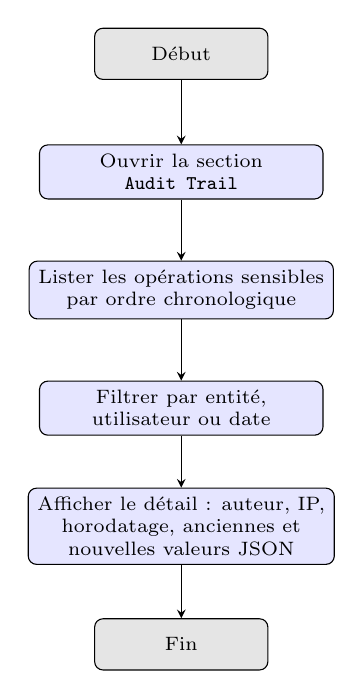
\begin{tikzpicture}[font=\scriptsize, >=stealth,
  startstop/.style={rectangle, rounded corners=3pt, fill=gray!20, draw=black, minimum width=2.2cm, minimum height=0.65cm, align=center},
  action/.style={rectangle, rounded corners=3pt, fill=blue!10, draw=black, minimum width=3.6cm, minimum height=0.65cm, align=center},
  decision/.style={diamond, draw=black, fill=orange!10, aspect=2, text width=2.6cm, align=center, inner sep=1pt},
  edgelabel/.style={font=\tiny, fill=white, inner sep=1pt}]

\node[startstop] (debut) at (0, 0) {D\'ebut};
\node[action] (ouvrir) at (0, -1.5) {Ouvrir la section\\\texttt{Audit Trail}};
\node[action] (lister) at (0, -3.0) {Lister les op\'erations sensibles\\par ordre chronologique};
\node[action] (filtrer) at (0, -4.5) {Filtrer par entit\'e,\\utilisateur ou date};
\node[action] (detail) at (0, -6.0) {Afficher le d\'etail : auteur, IP,\\horodatage, anciennes et\\nouvelles valeurs JSON};
\node[startstop] (fin) at (0, -7.5) {Fin};

\draw[->] (debut) -- (ouvrir);
\draw[->] (ouvrir) -- (lister);
\draw[->] (lister) -- (filtrer);
\draw[->] (filtrer) -- (detail);
\draw[->] (detail) -- (fin);
\end{tikzpicture}
  \end{LTR}
  \caption{مخطط النشاط : سجل التدقيق الأمني الشامل}
  \label{fig:act-13}
\end{figure}


\section{النمذجة الحركية (مخططات التسلسل)}
توضح مخططات التسلسل التالية الترتيب الزمني للرسائل المتبادلة بين الكائنات لتنفيذ أهم العمليات:

\subsection{مخطط تسلسل المصادقة والتحقق من الصلاحيات}
\begin{figure}[H]
  \centering
  \begin{LTR}
  \begin{tikzpicture}[>=Stealth,
    line/.style={dashed, color=gray!60, line width=0.5pt},
    actor/.style={draw=blue!70!black, fill=blue!10, rounded corners=3pt, minimum width=2.4cm, minimum height=0.8cm, align=center, font=\scriptsize\bfseries},
    sys/.style={draw=orange!80!black, fill=orange!10, rounded corners=3pt, minimum width=2.4cm, minimum height=0.8cm, align=center, font=\scriptsize\bfseries},
    db/.style={draw=gray!70!black, fill=gray!15, rounded corners=3pt, minimum width=2.4cm, minimum height=0.8cm, align=center, font=\scriptsize\bfseries},
    actbar/.style={fill=blue!30, draw=blue!50!black, line width=0.3pt},
    msg/.style={->, thick, >=Stealth, font=\scriptsize},
    reply/.style={<-, dashed, thick, >=Stealth, font=\scriptsize},
    mlabel/.style={above, fill=white, inner sep=1.5pt, font=\scriptsize},
    selfboxsys/.style={draw=orange!80!black, fill=orange!10, rounded corners=2pt, minimum height=0.55cm, align=center, inner sep=2pt, font=\scriptsize}
]
\node[actor] (u) at (0,0) {Utilisateur};
\node[sys] (c) at (5,0) {Syst\`eme / Auth Controller};
\node[db] (d) at (10,0) {Base MySQL};

\draw[line] (0,-0.4) -- (0,-5.4);
\draw[line] (5,-0.4) -- (5,-5.4);
\draw[line] (10,-0.4) -- (10,-5.4);

% Activation bars
\draw[actbar] (-0.06,-1) rectangle (0.06,-4.6);
\draw[actbar] (4.94,-1) rectangle (5.06,-4.6);
\draw[actbar] (9.94,-1.9) rectangle (10.06,-2.8);

% Messages
\draw[msg] (0,-1) -- node[mlabel] {1. POST /login (email, password)} (5,-1);
\draw[msg] (5,-1.9) -- node[mlabel] {2. SELECT user by email} (10,-1.9);
\draw[reply] (5,-2.8) -- node[mlabel] {3. User record \& hash} (10,-2.8);
\node[selfboxsys, anchor=west] (self4) at (5.4,-3.7) {4. V\'erification Hash \& R\^ole};
\draw[msg] (5,-3.7) -- (self4.west);
\draw[reply] (0,-4.6) -- node[mlabel] {5. Redirection Dashboard selon R\^ole} (5,-4.6);
\end{tikzpicture}
  \end{LTR}
  \caption{مخطط التسلسل : عملية المصادقة وتوجيه الجلسة}
  \label{fig:seq-auth}
\end{figure}

\subsection{مخطط تسلسل تقديم الطلب والتأهيل التجاري}
\begin{figure}[H]
  \centering
  \begin{LTR}
  \begin{tikzpicture}[>=Stealth,
    line/.style={dashed, color=gray!60, line width=0.5pt},
    actor/.style={draw=blue!70!black, fill=blue!10, rounded corners=3pt, minimum width=2.4cm, minimum height=0.8cm, align=center, font=\scriptsize\bfseries},
    sys/.style={draw=orange!80!black, fill=orange!10, rounded corners=3pt, minimum width=2.4cm, minimum height=0.8cm, align=center, font=\scriptsize\bfseries},
    actbar/.style={fill=blue!30, draw=blue!50!black, line width=0.3pt},
    msg/.style={->, thick, >=Stealth, font=\scriptsize},
    reply/.style={<-, dashed, thick, >=Stealth, font=\scriptsize},
    mlabel/.style={above, fill=white, inner sep=1.5pt, font=\scriptsize}
]
\node[actor] (cl) at (0,0) {Client};
\node[sys] (app) at (5.5,0) {Plateforme Web};
\node[actor] (co) at (11,0) {Commercial};

\draw[line] (0,-0.4) -- (0,-5.4);
\draw[line] (5.5,-0.4) -- (5.5,-5.4);
\draw[line] (11,-0.4) -- (11,-5.4);

% Activation bars
\draw[actbar] (-0.06,-1) rectangle (0.06,-4.6);
\draw[actbar] (5.44,-1) rectangle (5.56,-4.6);
\draw[actbar] (10.94,-1.9) rectangle (11.06,-3.7);

% Messages
\draw[msg] (0,-1) -- node[mlabel] {1. Soumission Demande Multi-\'Equipements} (5.5,-1);
\draw[msg] (5.5,-1.9) -- node[mlabel] {2. Notification nouvelle demande} (11,-1.9);
\draw[msg] (11,-2.8) -- node[mlabel] {3. Qualification \& Association Services} (5.5,-2.8);
\draw[msg] (11,-3.7) -- node[mlabel] {4. \'Emission du Devis / Contrat} (5.5,-3.7);
\draw[reply] (0,-4.6) -- node[mlabel] {5. Notification Devis disponible} (5.5,-4.6);
\end{tikzpicture}
  \end{LTR}
  \caption{مخطط التسلسل : تقديم الطلب ودراسته التجارية}
  \label{fig:seq-request}
\end{figure}

\subsection{مخطط تسلسل تنفيذ المعايرة، رفع التقرير والمراجعة}
\begin{figure}[H]
  \centering
  \begin{LTR}
  \begin{tikzpicture}[>=Stealth,
    line/.style={dashed, color=gray!60, line width=0.5pt},
    actor/.style={draw=blue!70!black, fill=blue!10, rounded corners=3pt, minimum width=2.4cm, minimum height=0.8cm, align=center, font=\scriptsize\bfseries},
    sys/.style={draw=orange!80!black, fill=orange!10, rounded corners=3pt, minimum width=2.4cm, minimum height=0.8cm, align=center, font=\scriptsize\bfseries},
    actbar/.style={fill=blue!30, draw=blue!50!black, line width=0.3pt},
    msg/.style={->, thick, >=Stealth, font=\scriptsize},
    reply/.style={<-, dashed, thick, >=Stealth, font=\scriptsize},
    mlabel/.style={above, fill=white, inner sep=1.5pt, font=\scriptsize},
    selfbox/.style={draw=blue!70!black, fill=blue!10, rounded corners=2pt, minimum height=0.55cm, align=center, inner sep=2pt, font=\scriptsize}
]
\node[actor] (m) at (0,0) {Responsable};
\node[sys] (app) at (5.3,0) {Syst\`eme};
\node[actor] (t) at (10.6,0) {Technicien};

\draw[line] (0,-0.4) -- (0,-6.3);
\draw[line] (5.3,-0.4) -- (5.3,-6.3);
\draw[line] (10.6,-0.4) -- (10.6,-6.3);

% Activation bars
\draw[actbar] (-0.06,-1) rectangle (0.06,-5.5);
\draw[actbar] (5.24,-1) rectangle (5.36,-5.5);
\draw[actbar] (10.54,-1.9) rectangle (10.66,-3.7);

% Messages
\draw[msg] (0,-1) -- node[mlabel] {1. Affectation de l'op\'eration} (5.3,-1);
\draw[msg] (5.3,-1.9) -- node[mlabel] {2. Notification t\^ache affect\'ee} (10.6,-1.9);
\node[selfbox, anchor=west] (self3) at (11.0,-2.8) {3. Prise en charge \& Mesures};
\draw[msg] (10.6,-2.8) -- (self3.west);
\draw[msg] (10.6,-3.7) -- node[mlabel] {4. T\'el\'eversement Rapport d'Essai (PDF)} (5.3,-3.7);
\draw[reply] (0,-4.6) -- node[mlabel] {5. Revue qualit\'e du rapport} (5.3,-4.6);
\draw[msg] (0,-5.5) -- node[mlabel] {6. Approbation ou Demande de Rework} (5.3,-5.5);
\end{tikzpicture}
  \end{LTR}
  \caption{مخطط التسلسل : التنفيذ المخبري ومراقبة الجودة}
  \label{fig:seq-calibration}
\end{figure}

\subsection{مخطط تسلسل الاعتماد النهائي للشهادة والتحميل}
\begin{figure}[H]
  \centering
  \begin{LTR}
  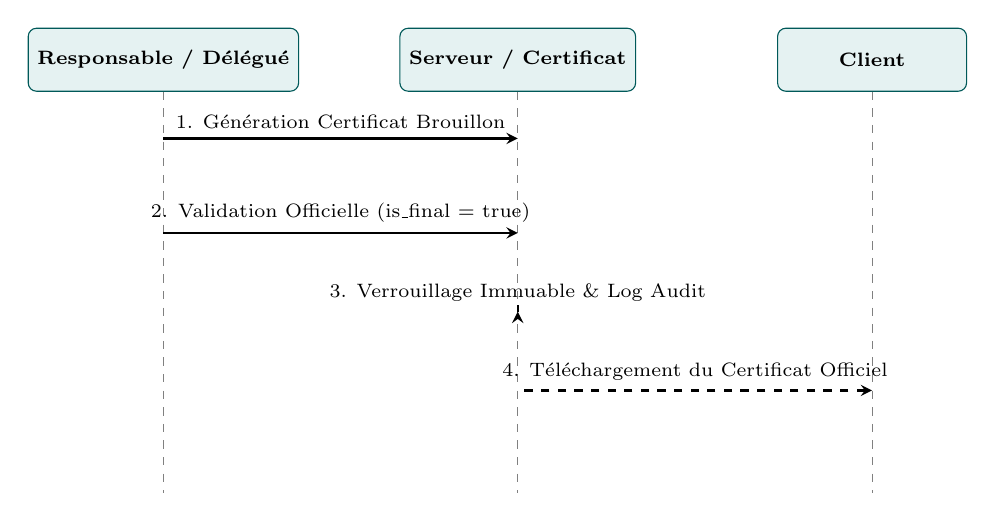
\begin{tikzpicture}[>=stealth,
    line/.style={dashed, color=gray},
    box/.style={draw=teal!70!black, fill=teal!10, rounded corners=3pt, minimum width=2.4cm, minimum height=0.8cm, align=center, font=\scriptsize\bfseries},
    msg/.style={->, thick, >=stealth, font=\scriptsize},
    reply/.style={<-, dashed, thick, >=stealth, font=\scriptsize}
]
\node[box] (m) at (0,0) {Responsable / D\'el\'egu\'e};
\node[box] (app) at (4.5,0) {Serveur / Certificat};
\node[box] (cl) at (9,0) {Client};

\draw[line] (m) -- (0,-5.5);
\draw[line] (app) -- (4.5,-5.5);
\draw[line] (cl) -- (9,-5.5);

\draw[msg] (0,-1) -- node[above] {1. G\'en\'eration Certificat Brouillon} (4.5,-1);
\draw[msg] (0,-2.2) -- node[above] {2. Validation Officielle (is\_final = true)} (4.5,-2.2);
\draw[msg] (4.5,-3.2) -- node[above] {3. Verrouillage Immuable \& Log Audit} (4.5,-3.2);
\draw[reply] (9,-4.2) -- node[above] {4. T\'el\'echargement du Certificat Officiel} (4.5,-4.2);
\end{tikzpicture}

  \end{LTR}
  \caption{مخطط التسلسل : تثبيت الشهادة وتحميلها للزبون}
  \label{fig:seq-certificate}
\end{figure}

\section{مخطط الحالات والانتقالات لدورة حياة الطلب}
تتغير حالة طلب المعايرة وفق دورة حياة منضبطة يوضحها مخطط الآلة ذات الحالات المنتهية التالي:

\begin{figure}[H]
  \centering
  \begin{LTR}
  \begin{tikzpicture}[
    >=Stealth,
    line width=0.8pt,
    state/.style={draw=blue!70!black, fill=blue!10, rounded corners=3pt, text width=4.3cm, align=center, minimum height=1.1cm, font=\footnotesize},
    terminal/.style={draw=red!70!black, fill=red!10, rounded corners=3pt, minimum width=2.8cm, align=center, font=\footnotesize},
    startnode/.style={circle, fill=black, minimum size=0.35cm, inner sep=0pt},
    endnode/.style={circle, draw=black, fill=black, minimum size=0.35cm, inner sep=0pt, double, double distance=1.5pt},
    arr/.style={->, >=Stealth, line width=0.8pt},
    lab/.style={font=\scriptsize, inner sep=1pt}
]
% --- \'etats : colonne gauche ---
\node[startnode] (init) at (0, 1.3) {};
\node[state] (s1)  at (0, 0)    {\textbf{Soumise}\\[2pt]\scriptsize\texttt{SUBMITTED}};
\node[state] (s2)  at (0, -2)   {\textbf{Transmise \`a la m\'etrologie}\\[2pt]\scriptsize\texttt{SENT\_TO\_METROLOGY}};
\node[state] (s3)  at (0, -4)   {\textbf{Date propos\'ee}\\[2pt]\scriptsize\texttt{DATE\_PROPOSED}};
\node[state] (s4)  at (0, -6)   {\textbf{En attente de confirmation du client}\\[2pt]\scriptsize\texttt{WAITING\_CLIENT\_CONFIRMATION}};
\node[state] (s5)  at (0, -8)   {\textbf{Accept\'ee}\\[2pt]\scriptsize\texttt{ACCEPTED}};
\node[state] (s6)  at (0, -10)  {\textbf{Sous contrat}\\[2pt]\scriptsize\texttt{CONTRACTED}};
\node[state] (s7)  at (0, -12)  {\textbf{Planifi\'ee}\\[2pt]\scriptsize\texttt{SCHEDULED}};

% --- \'etats : colonne droite ---
\node[state] (s8)  at (6.8, -12) {\textbf{Affect\'ee}\\[2pt]\scriptsize\texttt{ASSIGNED}};
\node[state] (s9)  at (6.8, -10) {\textbf{En cours de calibration}\\[2pt]\scriptsize\texttt{IN\_CALIBRATION}};
\node[state] (s10) at (6.8, -8)  {\textbf{Rapport t\'el\'evers\'e}\\[2pt]\scriptsize\texttt{REPORT\_UPLOADED}};
\node[state] (s11) at (6.8, -6)  {\textbf{En attente de certificat}\\[2pt]\scriptsize\texttt{WAITING\_CERTIFICATE}};
\node[state] (s12) at (6.8, -4)  {\textbf{Certificat g\'en\'er\'e}\\[2pt]\scriptsize\texttt{CERTIFICATE\_GENERATED}};
\node[state] (s13) at (6.8, -2)  {\textbf{Certificat valid\'e}\\[2pt]\scriptsize\texttt{CERTIFICATE\_VALIDATED}};
\node[state] (s14) at (6.8, 0)   {\textbf{Termin\'ee}\\[2pt]\scriptsize\texttt{COMPLETED}};

% --- \'etats terminaux ---
\node[terminal, minimum height=1.8cm] (rej) at (-4.6, -1) {\textbf{Rejet\'ee}\\[2pt]\scriptsize\texttt{REJECTED}};
\node[terminal, minimum height=3.2cm] (can) at (-4.6, -6) {\textbf{Annul\'ee}\\[2pt]\scriptsize\texttt{CANCELLED}};

\node[endnode] (fin) at (6.8, 1.3) {};

% --- transition initiale ---
\draw[arr] (init) -- (s1.north);
\node[lab] at (0.25, 1.0) {Soumission de la demande};

% --- chemin nominal : colonne gauche ---
\draw[arr] (s1) -- node[lab, right] {Transmission \`a la m\'etrologie} (s2);
\draw[arr] (s2) -- node[lab, right] {Proposition de date} (s3);
\draw[arr] (s3) -- node[lab, right] {En attente de l'accord client} (s4);
\draw[arr] (s4) -- node[lab, right] {Accord du client} (s5);
\draw[arr] (s5) -- node[lab, right] {Signature du contrat} (s6);
\draw[arr] (s6) -- node[lab, right] {Planification} (s7);

% --- chemin nominal : liaison basse ---
\draw[arr] (s7) -- node[lab, above] {Affectation du technicien} (s8);

% --- chemin nominal : colonne droite ---
\draw[arr] (s8)  -- node[lab, right] {D\'ebut de la calibration} (s9);
\draw[arr] (s9)  -- node[lab, right] {T\'el\'eversement du rapport} (s10);
\draw[arr] (s10) -- node[lab, right] {Attente du certificat} (s11);
\draw[arr] (s11) -- node[lab, right] {G\'en\'eration du certificat} (s12);
\draw[arr] (s12) -- node[lab, right] {Validation du certificat} (s13);
\draw[arr] (s13) -- node[lab, right] {Certificat immuable} (s14);

% --- transition finale ---
\draw[arr] (s14.north) -- (fin);

% --- boucle de correction du rapport ---
\draw[arr] (s10.west) -- (4.2, -8) -- (4.2, -10) -- (s9.west);
\node[lab] at (4.3, -9) {Rapport \`a corriger};

% --- rejet ---
\draw[arr] (s1.west) -- (-3.2, 0) -- (-3.2, -0.2);
\node[lab] at (-2.5, 0.15) {Rejet};
\draw[arr] (s2.west) -- (-3.2, -2) -- (-3.2, -1.8);
\node[lab] at (-2.5, -1.85) {Rejet};

% --- annulation ---
\draw[arr] (s3.west) -- (-3.2, -4) -- (-3.2, -4.6);
\node[lab] at (-2.5, -3.85) {Annulation};
\draw[arr] (s4.west) -- (-3.2, -6);
\node[lab] at (-2.5, -5.85) {Annulation};
\draw[arr] (s5.west) -- (-3.2, -8) -- (-3.2, -7.4);
\node[lab] at (-2.5, -7.85) {Annulation};
\end{tikzpicture}
  \end{LTR}
  \caption{مخطط الحالات والانتقالات لدورة حياة طلب المعايرة}
  \label{fig:state-request}
\end{figure}

\section{قواعد التسيير والترميز الموحد}
\subsection{قواعد الترميز الرسمي للوثائق}
تعتمد المنصة نظام ترميز موحداً يضمن تفرد كل وثيقة في قاعدة البيانات ويحافظ على إمكانية التتبع الكامل للمستندات. يوضح الجدول التالي تنسيق كل مرجع مع تفسير مكوناته ومثال تطبيقي:

\begin{codiftablear}{ترميز المراجع الرسمية للوثائق}
  \codifrowar{REQ-\textit{YYYY}-\textit{XXXX}}{مرجع طلب المعايرة: السنة (YYYY) ثم رقم تسلسلي من 4 أرقام}{REQ-2026-0012}
  \codifrowar{DEV-\textit{YYYY}-\textit{XXXX}}{مرجع الفاتورة التقديرية (الدراسة التجارية)}{DEV-2026-0012}
  \codifrowar{CTR-\textit{YYYY}-\textit{XXXX}}{مرجع العقد الموقع مع الزبون}{CTR-2026-0008}
  \codifrowar{CERT-\textit{DOM}-\textit{YYYY}-\textit{XXXXX}}{رقم شهادة المعايرة: رمز المجال، السنة، ثم رقم من 5 أرقام}{CERT-PRES-2026-00045}
  \codifrowar{ETL-\textit{DOM}-\textit{SERIE}}{رمز العتاد المرجعي المخبري (المجال + الرقم التسلسلي)}{ETL-PRES-WIKA-01}
  \codifrowar{SRV-\textit{DOM}-\textit{NN}}{رمز خدمة المعايرة في الدليل (المجال + تسلسل)}{SRV-PRES-01}
\end{codiftablear}

\subsection{قواعد التسيير المعتمدة (RG)}
\begin{itemize}
  \item \textbf{RG1 (تعدد المعدات) :} يجب أن يحتوي طلب المعايرة على معدة قياس واحدة على الأقل ($1..*$).
  \item \textbf{RG2 (تأكيد الموعد) :} يمنع الشروع في معايرة أي معدة قبل مصادقة الزبون الصريحة على تاريخ ومكان التدخل.
  \item \textbf{RG3 (تأهيل التقني) :} يشترط في التقني المترولوجي أن يكون حاصلاً على تأهيل معتمد في المجال الفيزيائي للأداة.
  \item \textbf{RG4 (تعليل التصحيح) :} كل قرار رفض لتقرير فني يوجب إدخال تبرير كتابي واضح يحدد النقائص التقنية المطلوبة للتصحيح.
  \item \textbf{RG5 (عدم قابلية تعديل الشهادات) :} بمجرد وضع علامة الاعتماد النهائي (\texttt{is\_final = true})، تصبح الشهادة محمية برمجياً ضد أي تعديل أو حذف في قاعدة البيانات.
  \item \textbf{RG6 (التفويض الموثق) :} في حال توقيع تقني مفوض بالنيابة عن المسؤول، يسجل النظام هويته وتاريخ التوقيع في سجل التدقيق الأمني.
  \item \textbf{RG7 (استبعاد العتاد المنتهي) :} يحظر النظام اختيار أي أداة عيارية مرجعية انتهت مدة صلاحيتها المخبرية.
\end{itemize}

\section{النمذجة الهيكلية وقاموس المعطيات}
\subsection{مخطط الفئات الخاص بالمجال المترولوجي}
يمثل مخطط الفئات التالي البنية الهيكلية لكائنات النظام وعلاقاتها:

\begin{figure}[H]
  \centering
  \begin{LTR}
  \begin{tikzpicture}[>=Stealth, line width=0.8pt,
    classbox/.style={draw=blue!70!black, fill=blue!10, rectangle, rounded corners=2pt,
        minimum width=3.6cm, align=left, font=\scriptsize, inner sep=3pt},
    assoc/.style={->, draw=blue!70!black, line width=0.8pt},
    mult/.style={font=\scriptsize}
]
% --- Row 1 : y = 9.5 ---
\node[classbox] (client) at (2, 9.5) {
\makebox[3.4cm][c]{\textbf{Client}}\\
\rule{3.4cm}{0.4pt}\\
+ id: int\\
+ company\_name: string\\
+ contact\_name: string\\
+ email: string\\
+ phone: string\\
+ tax\_id: string\\
\rule{3.4cm}{0.4pt}\\
+ createRequest()\\
+ manageContracts()
};

\node[classbox] (req) at (8, 9.5) {
\makebox[3.4cm][c]{\textbf{CalibrationRequest}}\\
\rule{3.4cm}{0.4pt}\\
+ id: int\\
+ request\_number: string\\
+ client\_id: int\\
+ status: string\\
+ scheduled\_date: date\\
+ location: string\\
\rule{3.4cm}{0.4pt}\\
+ items()\\
+ operations()\\
+ quotations()\\
+ schedule()
};

\node[classbox] (item) at (14, 9.5) {
\makebox[3.4cm][c]{\textbf{CalibrationRequestItem}}\\
\rule{3.4cm}{0.4pt}\\
+ id: int\\
+ equipment\_name: string\\
+ serial\_number: string\\
+ tolerance: string\\
+ quantity: int\\
\rule{3.4cm}{0.4pt}\\
+ validateTolerance()
};

% --- Row 2 : y = 4.5 ---
\node[classbox] (rep) at (2, 4.5) {
\makebox[3.4cm][c]{\textbf{CalibrationReport}}\\
\rule{3.4cm}{0.4pt}\\
+ id: int\\
+ report\_number: string\\
+ calibration\_operation\_id: int\\
+ file\_path: string\\
+ status: string\\
+ review\_notes: text\\
\rule{3.4cm}{0.4pt}\\
+ submit()\\
+ approve()\\
+ requestRework()
};

\node[classbox] (op) at (8, 4.5) {
\makebox[3.4cm][c]{\textbf{CalibrationOperation}}\\
\rule{3.4cm}{0.4pt}\\
+ id: int\\
+ operation\_number: string\\
+ calibration\_request\_id: int\\
+ technician\_id: int\\
+ status: string\\
\rule{3.4cm}{0.4pt}\\
+ assign()\\
+ start()\\
+ complete()
};

\node[classbox] (service) at (14, 4.5) {
\makebox[3.4cm][c]{\textbf{CalibrationService}}\\
\rule{3.4cm}{0.4pt}\\
+ id: int\\
+ code: string\\
+ name: string\\
+ measurement\_category: string\\
+ unit\_price: decimal\\
\rule{3.4cm}{0.4pt}\\
+ listByDomain()\\
+ updatePrice()
};

% --- Row 3 : y = -0.5 ---
\node[classbox] (user) at (2, -0.5) {
\makebox[3.4cm][c]{\textbf{User}}\\
\rule{3.4cm}{0.4pt}\\
+ id: int\\
+ name: string\\
+ email: string\\
+ role: string\\
+ is\_delegated\_manager: bool\\
+ client\_id: int\\
\rule{3.4cm}{0.4pt}\\
+ hasRole()\\
+ can()
};

\node[classbox] (cert) at (8, -0.5) {
\makebox[3.4cm][c]{\textbf{CalibrationCertificate}}\\
\rule{3.4cm}{0.4pt}\\
+ id: int\\
+ certificate\_number: string\\
+ calibration\_operation\_id: int\\
+ is\_final: bool\\
+ validated\_by: int\\
\rule{3.4cm}{0.4pt}\\
+ generate()\\
+ validate()\\
+ lock()
};

% --- Associations ---
\draw[assoc] (client.east) -- node[above, mult] {1} node[above, mult, pos=0.85] {0..*} (req.west);
\draw[assoc] (req.east) -- node[above, mult] {1} node[above, mult, pos=0.85] {1..*} (item.west);
\draw[assoc] (item.south) -- node[left, mult, pos=0.25] {1..*} node[left, mult, pos=0.75] {1} (service.north);
\draw[assoc] (req.south) -- node[right, mult, pos=0.25] {1} node[right, mult, pos=0.75] {0..*} (op.north);
\draw[assoc] (op.west) -- node[above, mult] {1} node[above, mult, pos=0.85] {0..1} (rep.east);
\draw[assoc] (op.south) -- node[right, mult, pos=0.25] {1} node[right, mult, pos=0.75] {0..1} (cert.north);
\draw[assoc] (item.south) -- (14, 6.9) -- (11, 6.9) -- (11, -0.5) -- node[above, mult, pos=0.9] {0..*} (cert.east);
\draw[assoc] (user.north) -- node[right, mult, pos=0.25] {1} node[right, mult, pos=0.75] {0..*} (rep.south);
\draw[assoc] (user.north) -- node[below, mult, pos=0.3] {1} node[below, mult, pos=0.85] {0..*} (op.south);
\end{tikzpicture}
  \end{LTR}
  \caption{مخطط فئات مجال المعايرة والمترولوجيا (Domain Class Diagram)}
  \label{fig:class-domain}
\end{figure}

\subsection{الجدول التركيبي للفئات الأساسية}
يلخص الجدول التالي أهم الخواص والأساليب السلوكية لكل فئة من فئات المجال:

\begin{summarytablear}{الجدول التركيبي للفئات الأساسية (Class Summary)}
  \summaryrowar{User}{id, name, email, password, role, is\_delegated\_manager, client\_id}{login(), logout(), assignRole()}
  \summaryrowar{Client}{id, company\_name, contact\_name, email, phone, tax\_id}{createRequest(), manageContracts()}
  \summaryrowar{CalibrationService}{id, code, name, domain, unit\_price}{listByDomain(), updatePrice()}
  \summaryrowar{CalibrationRequest}{id, reference, client\_id, status, scheduled\_date, location}{submit(), schedule(), statusFlow()}
  \summaryrowar{RequestItem}{id, request\_id, service\_id, name, serial, tolerance}{validateTolerance()}
  \summaryrowar{Quotation}{id, reference, request\_id, total\_ht, tva\_rate, total\_ttc}{computeTotals(), approve()}
  \summaryrowar{Contract}{id, contract\_number, client\_id, start\_date, end\_date}{archive()}
  \summaryrowar{CalibrationOperation}{id, request\_id, technician\_id, status}{assign(), start(), complete()}
  \summaryrowar{CalibrationReport}{id, operation\_id, file\_path, status, rejection\_reason}{submit(), approve(), requestRework()}
  \summaryrowar{Certificate}{id, number, operation\_id, is\_draft, is\_final}{generate(), validate(), lock()}
  \summaryrowar{MetrologyMaterial}{id, code, name, calibration\_date, expiration\_date}{checkValidity(), alertIfExpired()}
  \summaryrowar{AuditLog}{id, user\_id, action, entity\_type, old\_values, new\_values}{record(), query()}
\end{summarytablear}

\subsection{قاموس المعطيات للجداول الأساسية}
فيما يلي البنية التفصيلية لأهم جداول قاعدة البيانات:

%% جدول المستخدمين
\begin{dbtablear}{قاموس معطيات جدول المستخدمين (users)}
  \dbcolar{id}{bigint unsigned}{لا}{المعرف الرقمي الفريد (مفتاح رئيسي)}
  \dbcolar{name}{varchar(255)}{لا}{الاسم الكامل للمستخدم}
  \dbcolar{email}{varchar(255)}{لا}{البريد الإلكتروني (اسم المستخدم الفريد)}
  \dbcolar{password}{varchar(255)}{لا}{كلمة المرور المشفرة بتجزئة bcrypt}
  \dbcolar{role}{varchar(50)}{لا}{الرتبة في النظام (زبون، تجاري، مسؤول، إلخ)}
  \dbcolar{is\_delegated\_manager}{boolean}{لا}{مؤشر حق التفويض في توقيع الشهادات}
  \dbcolar{client\_id}{bigint unsigned}{نعم}{مفتاح أجنبي يربط المستخدم بمؤسسته}
\end{dbtablear}

%% جدول المؤسسات
\begin{dbtablear}{قاموس معطيات جدول المؤسسات والزبائن (clients)}
  \dbcolar{id}{bigint unsigned}{لا}{المعرف الفريد للمؤسسة}
  \dbcolar{company\_name}{varchar(255)}{لا}{التسمية الرسمية للشركة}
  \dbcolar{contact\_name}{varchar(255)}{لا}{اسم ولقب المسؤول المخول}
  \dbcolar{email}{varchar(255)}{لا}{البريد الإلكتروني للاتصال المهني}
  \dbcolar{phone}{varchar(50)}{لا}{رقم الهاتف الرسمي}
  \dbcolar{tax\_id}{varchar(100)}{نعم}{رقم التعريف الجبائي (NIF)}
\end{dbtablear}

%% جدول طلبات المعايرة
\begin{dbtablear}{قاموس معطيات جدول طلبات المعايرة (calibration\_requests)}
  \dbcolar{id}{bigint unsigned}{لا}{المعرف الفريد للطلب}
  \dbcolar{reference}{varchar(50)}{لا}{المرجع الرقمي للطلب (REQ-YYYY-XXXX)}
  \dbcolar{client\_id}{bigint unsigned}{لا}{مفتاح أجنبي يشير إلى الزبون صاحب الطلب}
  \dbcolar{status}{varchar(50)}{لا}{الحالة الحالية للطلب في مسار المعايرة}
  \dbcolar{scheduled\_date}{date}{نعم}{التاريخ المتفق عليه للتدخل}
  \dbcolar{location}{varchar(20)}{لا}{مكان التدخل (المخبر أو موقع الزبون)}
\end{dbtablear}

%% جدول شهادات المعايرة
\begin{dbtablear}{قاموس معطيات جدول الشهادات الرسمية (calibration\_certificates)}
  \dbcolar{id}{bigint unsigned}{لا}{المعرف الفريد للشهادة}
  \dbcolar{certificate\_number}{varchar(50)}{لا}{الرقم الرسمي المرجعي لشهادة المعايرة}
  \dbcolar{calibration\_operation\_id}{bigint unsigned}{لا}{مفتاح أجنبي يربط الشهادة بعملية الفحص}
  \dbcolar{is\_draft}{boolean}{لا}{مؤشر المسودة المؤقتة للشهادة}
  \dbcolar{is\_final}{boolean}{لا}{قفل عدم قابلية التعديل النهائي}
  \dbcolar{validated\_by}{bigint unsigned}{نعم}{معرف المسؤول الذي وقع الشهادة}
  \dbcolar{validated\_at}{timestamp}{نعم}{التوقيت الدقيق لاعتماد وتثبيت الشهادة}
\end{dbtablear}

%% جدول خدمات المعايرة
\begin{dbtablear}{قاموس معطيات جدول خدمات المعايرة (calibration\_services)}
  \dbcolar{id}{bigint unsigned}{لا}{المعرف الفريد للخدمة}
  \dbcolar{code}{varchar(50)}{لا}{رمز الخدمة في الدليل (SRV-DOM-NN)}
  \dbcolar{name}{varchar(255)}{لا}{التسمية الرسمية للخدمة}
  \dbcolar{domain}{varchar(50)}{لا}{المجال الفيزيائي (الضغط، الحرارة، الكهرباء...)}
  \dbcolar{unit\_price}{decimal(10,2)}{لا}{التعرفة الفردية دون رسوم}
  \dbcolar{description}{text}{نعم}{الوصف التقني للخدمة}
\end{dbtablear}

%% جدول عناصر الطلب (المعدات)
\begin{dbtablear}{قاموس معطيات جدول عناصر الطلب والعتاد (calibration\_request\_items)}
  \dbcolar{id}{bigint unsigned}{لا}{المعرف الفريد للعنصر}
  \dbcolar{calibration\_request\_id}{bigint unsigned}{لا}{مفتاح أجنبي يشير إلى الطلب الأب}
  \dbcolar{calibration\_service\_id}{bigint unsigned}{نعم}{مفتاح أجنبي يشير إلى الخدمة المطابقة}
  \dbcolar{equipment\_name}{varchar(255)}{لا}{تسمية الجهاز المراد معايرته}
  \dbcolar{serial\_number}{varchar(100)}{لا}{الرقم التسلسلي عند الصانع}
  \dbcolar{brand}{varchar(100)}{نعم}{العلامة التجارية}
  \dbcolar{model}{varchar(100)}{نعم}{الطراز}
  \dbcolar{measurement\_range}{varchar(100)}{نعم}{نطاق القياس (مثال 0-250 bar)}
  \dbcolar{tolerance}{varchar(100)}{نعم}{الحدود المسموحة (مثال ±0.5\%)}
  \dbcolar{quantity}{int}{لا}{الكمية المطلوبة (الافتراضي 1)}
\end{dbtablear}

%% جدول الفواتير التقديرية
\begin{dbtablear}{قاموس معطيات جدول الفواتير التقديرية (quotations)}
  \dbcolar{id}{bigint unsigned}{لا}{المعرف الفريد للفاتورة}
  \dbcolar{reference}{varchar(50)}{لا}{المرجع الرسمي (DEV-YYYY-XXXX)}
  \dbcolar{calibration\_request\_id}{bigint unsigned}{لا}{مفتاح أجنبي يربط الفاتورة بالطلب}
  \dbcolar{total\_ht}{decimal(12,2)}{لا}{المجموع الكلي دون رسوم}
  \dbcolar{tva\_rate}{decimal(5,2)}{لا}{نسبة الرسم على القيمة المضافة 19\%}
  \dbcolar{total\_ttc}{decimal(12,2)}{لا}{المجموع الكلي شاملاً الأعباء}
  \dbcolar{status}{varchar(30)}{لا}{الحالة (مسودة، مرسلة، مقبولة)}
\end{dbtablear}

%% جدول العقود
\begin{dbtablear}{قاموس معطيات جدول العقود (contracts)}
  \dbcolar{id}{bigint unsigned}{لا}{المعرف الفريد للعقد}
  \dbcolar{contract\_number}{varchar(50)}{لا}{رقم العقد الإطاري}
  \dbcolar{client\_id}{bigint unsigned}{لا}{مفتاح أجنبي يشير إلى الزبون المتعاقد}
  \dbcolar{start\_date}{date}{لا}{تاريخ بداية سريان العقد}
  \dbcolar{end\_date}{date}{لا}{تاريخ انتهاء العقد}
  \dbcolar{status}{varchar(30)}{لا}{حالة العقد (نشط، مؤرشف)}
\end{dbtablear}

%% جدول عمليات المعايرة
\begin{dbtablear}{قاموس معطيات جدول عمليات المعايرة (calibration\_operations)}
  \dbcolar{id}{bigint unsigned}{لا}{المعرف الفريد للعملية}
  \dbcolar{calibration\_request\_id}{bigint unsigned}{لا}{مفتاح أجنبي يشير إلى الطلب الأب}
  \dbcolar{technician\_id}{bigint unsigned}{نعم}{مفتاح أجنبي يشير إلى التقني المكلف}
  \dbcolar{assigned\_by}{bigint unsigned}{نعم}{مفتاح أجنبي يشير إلى المسؤول الموكل}
  \dbcolar{status}{varchar(50)}{لا}{الحالة (مكلفة، قيد الإنجاز، منجزة)}
  \dbcolar{started\_at}{timestamp}{نعم}{لحظة بدء القياسات}
  \dbcolar{completed\_at}{timestamp}{نعم}{لحظة إتمام القياسات}
\end{dbtablear}

%% جدول تقارير المعايرة
\begin{dbtablear}{قاموس معطيات جدول التقارير الفنية (calibration\_reports)}
  \dbcolar{id}{bigint unsigned}{لا}{المعرف الفريد للتقرير}
  \dbcolar{calibration\_operation\_id}{bigint unsigned}{لا}{مفتاح أجنبي يربط التقرير بالعملية}
  \dbcolar{file\_path}{varchar(500)}{لا}{مسار التخزين الآمن للملف}
  \dbcolar{file\_name}{varchar(255)}{لا}{الاسم الأصلي للملف}
  \dbcolar{status}{varchar(30)}{لا}{الحالة (مقدم، مقبول، مرفوض)}
  \dbcolar{rejection\_reason}{text}{نعم}{التعليل الإجباري عند طلب التصحيح}
  \dbcolar{reviewed\_by}{bigint unsigned}{نعم}{المسؤول الذي أجرى المراجعة النوعية}
  \dbcolar{reviewed\_at}{timestamp}{نعم}{وقت المراجعة النوعية}
\end{dbtablear}

%% جدول العتاد المرجعي
\begin{dbtablear}{قاموس معطيات جدول العتاد المرجعي (metrology\_materials)}
  \dbcolar{id}{bigint unsigned}{لا}{المعرف الفريد للعتاد}
  \dbcolar{code}{varchar(50)}{لا}{الرمز الداخلي (ETL-DOM-SERIE)}
  \dbcolar{name}{varchar(255)}{لا}{تسمية الأداة المرجعية}
  \dbcolar{serial\_number}{varchar(100)}{لا}{الرقم التسلسلي للمعايرة}
  \dbcolar{calibration\_date}{date}{لا}{تاريخ آخر رصد مترولوجي}
  \dbcolar{expiration\_date}{date}{لا}{نهاية صلاحية الاستعمال المخبري}
  \dbcolar{status}{varchar(30)}{لا}{الحالة (صالح، منتهي، خارج الخدمة)}
\end{dbtablear}

%% جدول سجل التدقيق
\begin{dbtablear}{قاموس معطيات جدول سجل التدقيق الأمني (audit\_logs)}
  \dbcolar{id}{bigint unsigned}{لا}{المعرف الفريد للسجل}
  \dbcolar{user\_id}{bigint unsigned}{نعم}{مفتاح أجنبي يشير إلى منفذ العملية}
  \dbcolar{action}{varchar(100)}{لا}{نوع العملية (إنشاء، تحديث، اعتماد...)}
  \dbcolar{entity\_type}{varchar(100)}{لا}{الكيان المتأثر (طلب، تقرير، شهادة)}
  \dbcolar{entity\_id}{bigint unsigned}{لا}{رقم الكيان المتأثر}
  \dbcolar{old\_values}{json}{نعم}{القيم السابقة بتنسيق JSON}
  \dbcolar{new\_values}{json}{نعم}{القيم الجديدة بتنسيق JSON}
  \dbcolar{ip\_address}{varchar(45)}{نعم}{عنوان IP الخاص بالمصدر}
\end{dbtablear}

\begin{figure}[H]
  \centering
  \begin{LTR}
  \begin{tikzpicture}[>=Stealth, line width=0.8pt,
    tbl/.style={draw=blue!70!black, fill=blue!10, rounded corners=2pt,
        text width=3.5cm, align=center, font=\scriptsize\bfseries, inner sep=2pt},
    conn/.style={-, draw=blue!70!black, line width=0.8pt}
]
% --- Row 1 : y = 8 ---
\node[tbl] (roles) at (3, 8) {roles};
\node[tbl] (perm_role) at (8.5, 8) {permission\_role};
\node[tbl] (perms) at (14, 8) {permissions};

% --- Row 2 : y = 6.5 ---
\node[tbl] (clients) at (3, 6.5) {clients};
\node[tbl] (reqs) at (8.5, 6.5) {calibration\_requests};
\node[tbl] (contracts) at (14, 6.5) {contracts};

% --- Row 3 : y = 5 ---
\node[tbl] (quotes) at (3, 5) {quotations};
\node[tbl] (items) at (8.5, 5) {calibration\_request\_items};
\node[tbl] (services) at (14, 5) {calibration\_services};

% --- Row 4 : y = 3.5 ---
\node[tbl] (ops) at (8.5, 3.5) {calibration\_operations};
\node[tbl] (reps) at (14, 3.5) {calibration\_reports};

% --- Row 5 : y = 2 ---
\node[tbl] (status) at (3, 2) {request\_status\_histories};
\node[tbl] (certs) at (8.5, 2) {calibration\_certificates};
\node[tbl] (materials) at (14, 2) {metrology\_materials};

% --- Row 6 : y = 0.5 ---
\node[tbl] (audit) at (3, 0.5) {audit\_logs};
\node[tbl] (users) at (8.5, 0.5) {users};
\node[tbl] (docs) at (14, 0.5) {documents};

% --- RBAC : roles / permissions ---
\draw[conn] (roles.east) -- (perm_role.west);
\draw[conn] (perm_role.east) -- (perms.west);
\draw[conn] (roles.east) -- (5.0, 8) -- (5.0, 0.7) -- (users.west);

% --- Commercial : clients / contracts / quotations ---
\draw[conn] (clients.east) -- (reqs.west);
\draw[conn] (clients.south) -- (3, 5.9) -- (14, 5.9) -- (contracts.south);
\draw[conn] (reqs.south) -- (7.0, 6.1) -- (7.0, 5.7) -- (3, 5.7) -- (quotes.north);

% --- Metrology : requests / items / services / operations ---
\draw[conn] (reqs.south) -- (reqs.south |- items.north);
\draw[conn] (reqs.south) -- (9.0, 6.1) -- (9.0, 5.6) -- (11, 5.6) -- (11, 3.7) -- (ops.east);
\draw[conn] (reqs.south) -- (7.5, 6.1) -- (7.5, 5.8) -- (5.5, 5.8) -- (5.5, 2) -- (status.east);
\draw[conn] (items.east) -- (services.west);
\draw[conn] (items.south) -- (ops.north);
\draw[conn] (items.south) -- (8.5, 4.4) -- (6.3, 4.4) -- (6.3, 2) -- (certs.west);
\draw[conn] (ops.east) -- (reps.west);
\draw[conn] (ops.south) -- (certs.north);
\draw[conn] (reps.west) -- (certs.east);

% --- Users : hub ---
\draw[conn] (users.west) -- (audit.east);
\draw[conn] (users.east) -- (docs.west);
\draw[conn] (users.north) -- (certs.south);
\draw[conn] (users.west) -- (status.east);
\draw[conn] (users.south) -- (8.5, -0.6) -- (1.0, -0.6) -- (1.0, 6.5) -- (clients.east);
\draw[conn] (users.east) -- (10.32, 0.5) -- (10.32, 1.2) -- (14, 1.2) -- (reps.south);
\draw[conn] (users.north) -- (8.5, 1.5) -- (10.6, 1.5) -- (10.6, 3.3) -- (ops.east);
\end{tikzpicture}
  \end{LTR}
  \caption{المخطط العلائقي لقاعدة البيانات MySQL}
  \label{fig:db-cluster}
\end{figure}

\section{الانتقال إلى النموذج العلائقي (Passage au Modèle Relationnel)}
\subsection{قواعد التحويل المعتمدة}
النموذج العلائقي يمثل تجسيداً قاعدياً لمخطط الفئات، ويتم التحويل وفق القواعد التالية:
\begin{itemize}
  \item \textbf{R1 — الفئة إلى جدول :} كل فئة من فئات المجال تتحول إلى جدول مستقل في قاعدة البيانات.
  \item \textbf{R2 — الخواص إلى أعمدة :} كل خاصية تصبح عموداً بنفس نوعها المحدد في المخطط المفاهيمي.
  \item \textbf{R3 — العلاقة 1..N :} تُضاف مفتاح أجنبي (\textit{FK}) داخل جدول الجهة المتعددة يشير إلى مفتاح الجهة المرتبطة.
  \item \textbf{R4 — العلاقة N..M :} تُترجم إلى جدول وسيط (Pivot) يحمل مفاتيح أجنبية للطرفين مع الصفات الوصفية الخاصة بها.
  \item \textbf{R5 — الوراثة :} أساسي نماذج (الزبون، التقني، المشرف) مستخلصة من الفئة الأم \textbf{User} بالاعتماد على ملاحظة الدور الجوهرية.
\end{itemize}

\subsection{جدول التحويل (Mapping Table)}
يلخص الجدول التالي تطبيقات هذه القواعد على فئات النظام:

\begin{relmapar}{جدول تحويل فئات UML إلى جداول SQL}
  \relmaprow{User}{users}{id}{client\_id}{إضافة العمود role للتفريق بين الأدوار}
  \relmaprow{Client}{clients}{id}{--}{خاصية client\_id في جدول المستخدمين تحقق رابط 1..*}
  \relmaprow{CalibrationService}{calibration\_services}{id}{--}{جدول مستقل لمحتوى الدليل المترولوجي}
  \relmaprow{CalibrationRequest}{calibration\_requests}{id}{client\_id}{رابط 1..N بين الزبون والطلبات}
  \relmaprow{RequestItem}{calibration\_request\_items}{id}{calibration\_request\_id, calibration\_service\_id}{عناصر الطلب؛ ترتبط بجدول الخدمة مفتاح أجنبي عند التأهيل}
  \relmaprow{Quotation}{quotations}{id}{calibration\_request\_id}{رابط 1..1 بين الطلب والفواتير}
  \relmaprow{Contract}{contracts}{id}{client\_id}{عقود إطارية مرتبطة بالزبون}
  \relmaprow{CalibrationOperation}{calibration\_operations}{id}{calibration\_request\_id, technician\_id, assigned\_by}{تدخل المفاتيح الأجنبية الثلاثة للتعيين والتتبع}
  \relmaprow{CalibrationReport}{calibration\_reports}{id}{calibration\_operation\_id, reviewed\_by}{التقرير مرتبط بالعملية وبالمراجع النوعي}
  \relmaprow{Certificate}{calibration\_certificates}{id}{calibration\_operation\_id, validated\_by}{الشهادة مرقمة وحرفياً قياسية}
  \relmaprow{MetrologyMaterial}{metrology\_materials}{id}{--}{العتاد المرجعي محدودية صلاحية مسجلة}
  \relmaprow{AuditLog}{audit\_logs}{id}{user\_id}{سجل التدقيق يستقبل مراجع فاعلي كل عملية}
\end{relmapar}

\subsection{جداول الربط (Pivot Tables)}
تُستعمل جداول الربط لتحويل علاقات التعدد إلى جداول مستقلة، خاصةً في التعريف التقني للعتاد:

\begin{pivotar}{جداول الربط في قاعدة البيانات}
  \pivotrow{طلب \LR{(\seqsplit{CalibrationRequest})} $\leftrightarrow$ خدمة \LR{(\seqsplit{CalibrationService})} والعتاد}{calibration\_request\_items}{calibration\_request\_id + calibration\_service\_id}{الجدول الوسيط يخزن أيضاً بيانات الجهاز: الرقم التسلسلي، الطراز، الدقة}
  \pivotrow{تقني \LR{(User)} $\leftrightarrow$ عملية \LR{(\seqsplit{CalibrationOperation})}}{calibration\_operations}{technician\_id + assigned\_by}{التعيين موثق عبر مفتاحي التقني والمسؤول}
  \pivotrow{مسؤول \LR{(User)} $\leftrightarrow$ شهادة \LR{(Certificate)}}{calibration\_certificates}{validated\_by}{تسجيل الموقع الرسمي على الشهادة النهائية}
\end{pivotar}

\section{مخطط النشر الفيزيائي للمنصة}
يعتمد النشر الفعلي للمنصة على خادم بيئة الإنتاج بحزمة \textbf{LEMP} المؤمنة بشهادة التشفير الرقمي SSL/TLS:

\begin{figure}[H]
  \centering
  \begin{LTR}
  \begin{tikzpicture}[>=Stealth,
    client/.style={draw=blue!70!black, fill=blue!10, rounded corners=3pt, line width=0.8pt, minimum width=3.6cm, minimum height=2.8cm, align=center, font=\footnotesize},
    server/.style={draw=gray!70, fill=gray!5, rounded corners=3pt, line width=0.8pt, minimum width=9.2cm, minimum height=4.8cm},
    header/.style={draw=gray!70, fill=gray!70, text=white, font=\small\bfseries, minimum width=9.2cm, minimum height=0.8cm, align=center},
    inner/.style={draw=blue!70!black, fill=blue!10, rounded corners=3pt, line width=0.8pt, minimum width=7.2cm, minimum height=0.8cm, align=center, font=\scriptsize},
    innerdb/.style={draw=orange!80!black, fill=orange!10, rounded corners=3pt, line width=0.8pt, minimum width=7.2cm, minimum height=0.8cm, align=center, font=\scriptsize},
    arr/.style={<->, line width=0.8pt, >=Stealth, color=darkgray}
]
\node[client] (client) at (0,0) {\textbf{Poste Client}\\[4pt]Navigateur Web moderne\\Chrome / Firefox / Edge};
\node[server] (server) at (9.2,0) {};
\node[header, anchor=north] (srvhead) at (server.north) {Serveur d'Application (LEMP)};
\node[inner] (nginx) at (9.2, 0.9) {Nginx Web Server / SSL};
\node[inner] (php) at (9.2, -0.2) {PHP 8.2-FPM / Laravel 12/13};
\node[innerdb] (mysql) at (9.2, -1.3) {SGBD MySQL 8.0+};
\draw[arr] (client.east) -- node[above, font=\scriptsize] {HTTPS (Port 443)} node[below, font=\scriptsize] {Protocole TLS 1.3} (server.west);
\end{tikzpicture}
  \end{LTR}
  \caption{مخطط النشر الفيزيائي للمنصة (LEMP Topology)}
  \label{fig:deployment}
\end{figure}

\section*{خاتمة الفصل الثالث}
قدم هذا الفصل نمذجة تحليلية وهندسية تفصيلية لنظام تسيير المعايرة، حددت سلوكه الحركي والبياني. وسيتناول الفصل الرابع كيفية تجسيد هذه التصاميم برمجياً واختبارها عملياً.


%% ============================================================
%% الفصل الرابع : الإنجاز والاختبارات
%% ============================================================
\chapter{الإنجاز والاختبارات}

\section*{مقدمة الفصل}
يمثل هذا الفصل الختامي تتويجاً لكافة المراحل النظرية والتصميمية السابقة، حيث يعرض الجانب التطبيقي الفعلي لمنظومة تسيير المعايرة. نستعرض في مستهله بيئة التطوير والأدوات البرمجية المعتمدة، وهيكلة ملفات المشروع، ثم نقدم كود التطبيق المخصص لحماية الشهادات وعزل الزبائن، ونستعرض واجهات المستخدم الرئيسية المنفذة، ونختتم بالتحقق التجريبي عبر عرض نتائج حزمة الاختبارات الآلية التي حققت نسبة نجاح 100\%.

\section{بيئة التطوير والأدوات المعتمدة}
تم إنجاز المنصة بالاعتماد على بيئة تطوير متكاملة ومعيارية:
\begin{itemize}
  \item \textbf{نظام التشغيل :} Linux Ubuntu 24.04 LTS كبيئة عمل آمنة ومطابقة لبيئة الخوادم السحابية.
  \item \textbf{لغة الخادم ومحركه :} PHP 8.2 مع تشغيل الملحقات الضرورية مثل \texttt{pdo\_mysql} و \texttt{openssl}.
  \item \textbf{مدير الحزم الخلفية :} \textbf{Composer 2.8} لتثبيت وإدارة مكتبات Laravel.
  \item \textbf{مدير حزم الواجهة الأمامية :} \textbf{Node.js v22} مع مدير الحزم NPM.
  \item \textbf{محرر الأكواد :} Visual Studio Code مع إضافات التدقيق اللغوي الآلي والتنسيق.
  \item \textbf{نظام إدارة الإصدارات :} Git لمتابعة التعديلات وضمان أمان الكود المصدري.
\end{itemize}

\section{الهيكلة البرمجية للمشروع}
تمت هيكلة المشروع وفق أفضل الممارسات المعتمدة في إطار العمل Laravel مع Inertia:

\begin{figure}[H]
  \centering
  \begin{LTR}
  \begin{tikzpicture}[>=Stealth,
    folder/.style={draw=blue!80!black, fill=blue!10, rounded corners=3pt, line width=0.8pt, minimum width=4.0cm, minimum height=0.7cm, align=center, font=\scriptsize\ttfamily},
    desc/.style={font=\scriptsize, align=left, text width=9cm}
]
\node[folder] (app) {app/};
\node[desc, right=0.5cm of app] (appdesc) {Logique m\'etier, Mod\`eles Eloquent, Services, Policies};

\node[folder, below=0.9cm of app] (http) {app/Http/Controllers/};
\node[desc, right=0.5cm of http] (httpdesc) {Contr\^oleurs d'orchestration (Inertia responses)};

\node[folder, below=0.9cm of http] (resources) {resources/js/Pages/};
\node[desc, right=0.5cm of resources] (resdesc) {Vues et composants React 19 / TypeScript};

\node[folder, below=0.9cm of resources] (routes) {routes/web.php};
\node[desc, right=0.5cm of routes] (routesdesc) {D\'efinition des routes prot\'eg\'ees par Middleware};

\node[folder, below=0.9cm of routes] (tests) {tests/Feature/};
\node[desc, right=0.5cm of tests] (testsdesc) {Suite de 67 tests Pest/PHPUnit (100\% couverture)};
\end{tikzpicture}
  \end{LTR}
  \caption{الهيكلة البرمجية للمشروع وتوزيع المجلدات والمسارات}
  \label{fig:app-structure}
\end{figure}

\subsection{تطبيق مبدأ عدم قابلية تعديل الشهادات (Immutability)}
تم تطبيق مبدأ الحظر الصارم لأي تعديل على الشهادات النهائية من خلال أحداث النموذج (\textit{Eloquent Model Events}) في الملف \texttt{app/Models/CalibrationCertificate.php}:
\begin{LTR}
\begin{verbatim}
protected static function booted(): void
{
    static::updating(function (CalibrationCertificate $cert) {
        if ($cert->getOriginal('is_final')) {
            throw new \DomainException(
                "This certificate is final and immutable. " .
                "Modification forbidden."
            );
        }
    });

    static::deleting(function (CalibrationCertificate $cert) {
        if ($cert->is_final) {
            throw new \DomainException(
                "Deleting a finalized calibration certificate " .
                "is forbidden."
            );
        }
    });
}
\end{verbatim}
\end{LTR}

\section{استعراض واجهات النظام الرئيسية}
\subsection{الواجهة العامة ودليل الخدمات المترولوجية}
تتيح للزوار والزبائن التعرف على المجالات الستة المعتمدة في المخبر، مع إمكانية البحث الفوري عن أدوات القياس ومعرفة شروط التكفل ومداها الفني.

\begin{figure}[H]
  \centering
  \begin{LTR}
  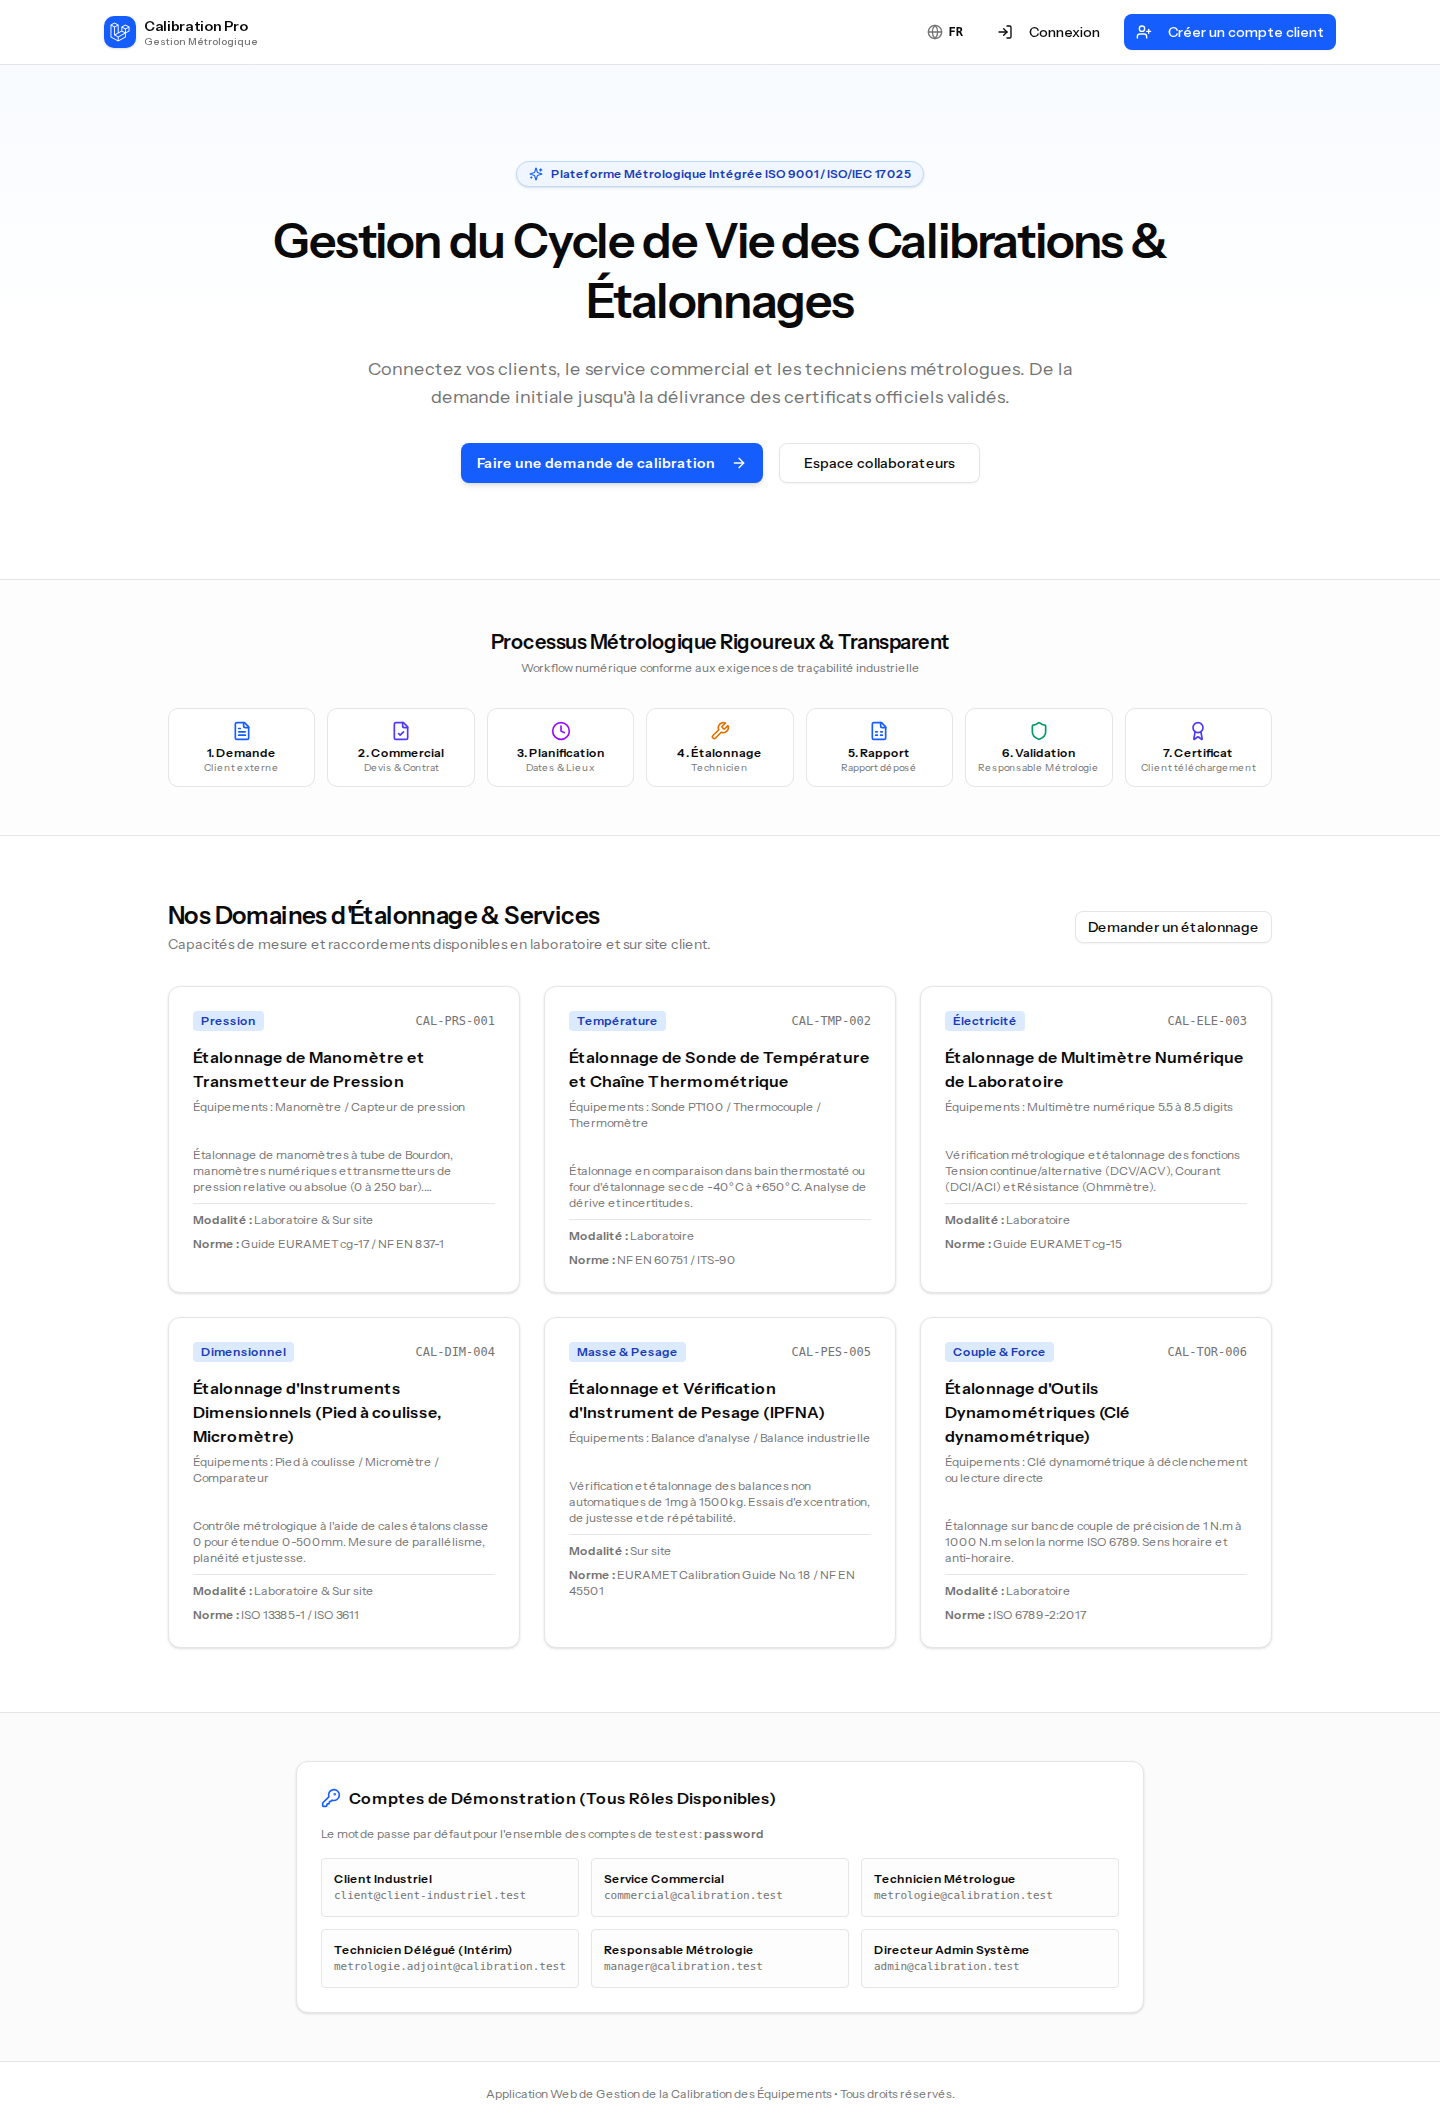
\includegraphics[width=0.9\linewidth]{figures/welcome.png}
  \end{LTR}
  \caption{الواجهة العامة للمنصة ودليل الخدمات المترولوجية}
  \label{fig:ui-welcome}
\end{figure}

\subsection{فضاء الزبون : إدراج طلب متعدد المعدات وتتبع الشهادات}
تسمح للزبون الصناعي بإضافة عدة أجهزة دفعة واحدة مع تحديد أرقامها التسلسلية وخصائصها، ومتابعة تغير حالة كل أداة خطوة بخطوة حتى تحميل شهادة المعايرة المعتمدة بنقرة واحدة.

\begin{figure}[H]
  \centering
  \begin{LTR}
  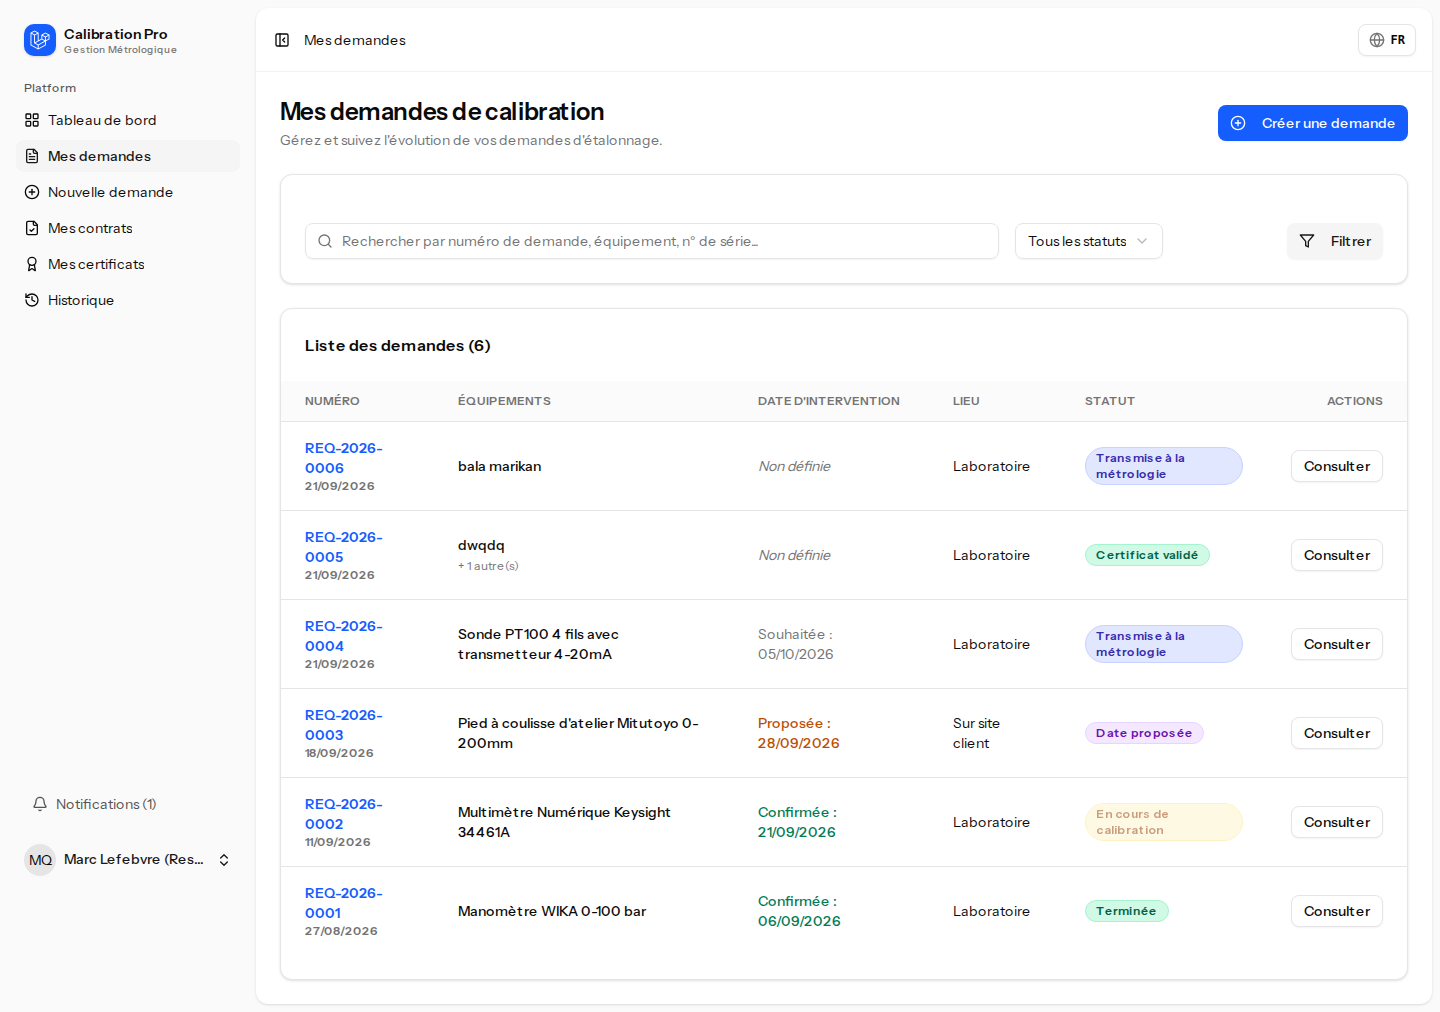
\includegraphics[width=0.9\linewidth]{figures/client-requests.png}
  \end{LTR}
  \caption{فضاء الزبون : قائمة الطلبات وتتبع حالات المعايرة}
  \label{fig:ui-client-requests}
\end{figure}

\begin{figure}[H]
  \centering
  \begin{LTR}
  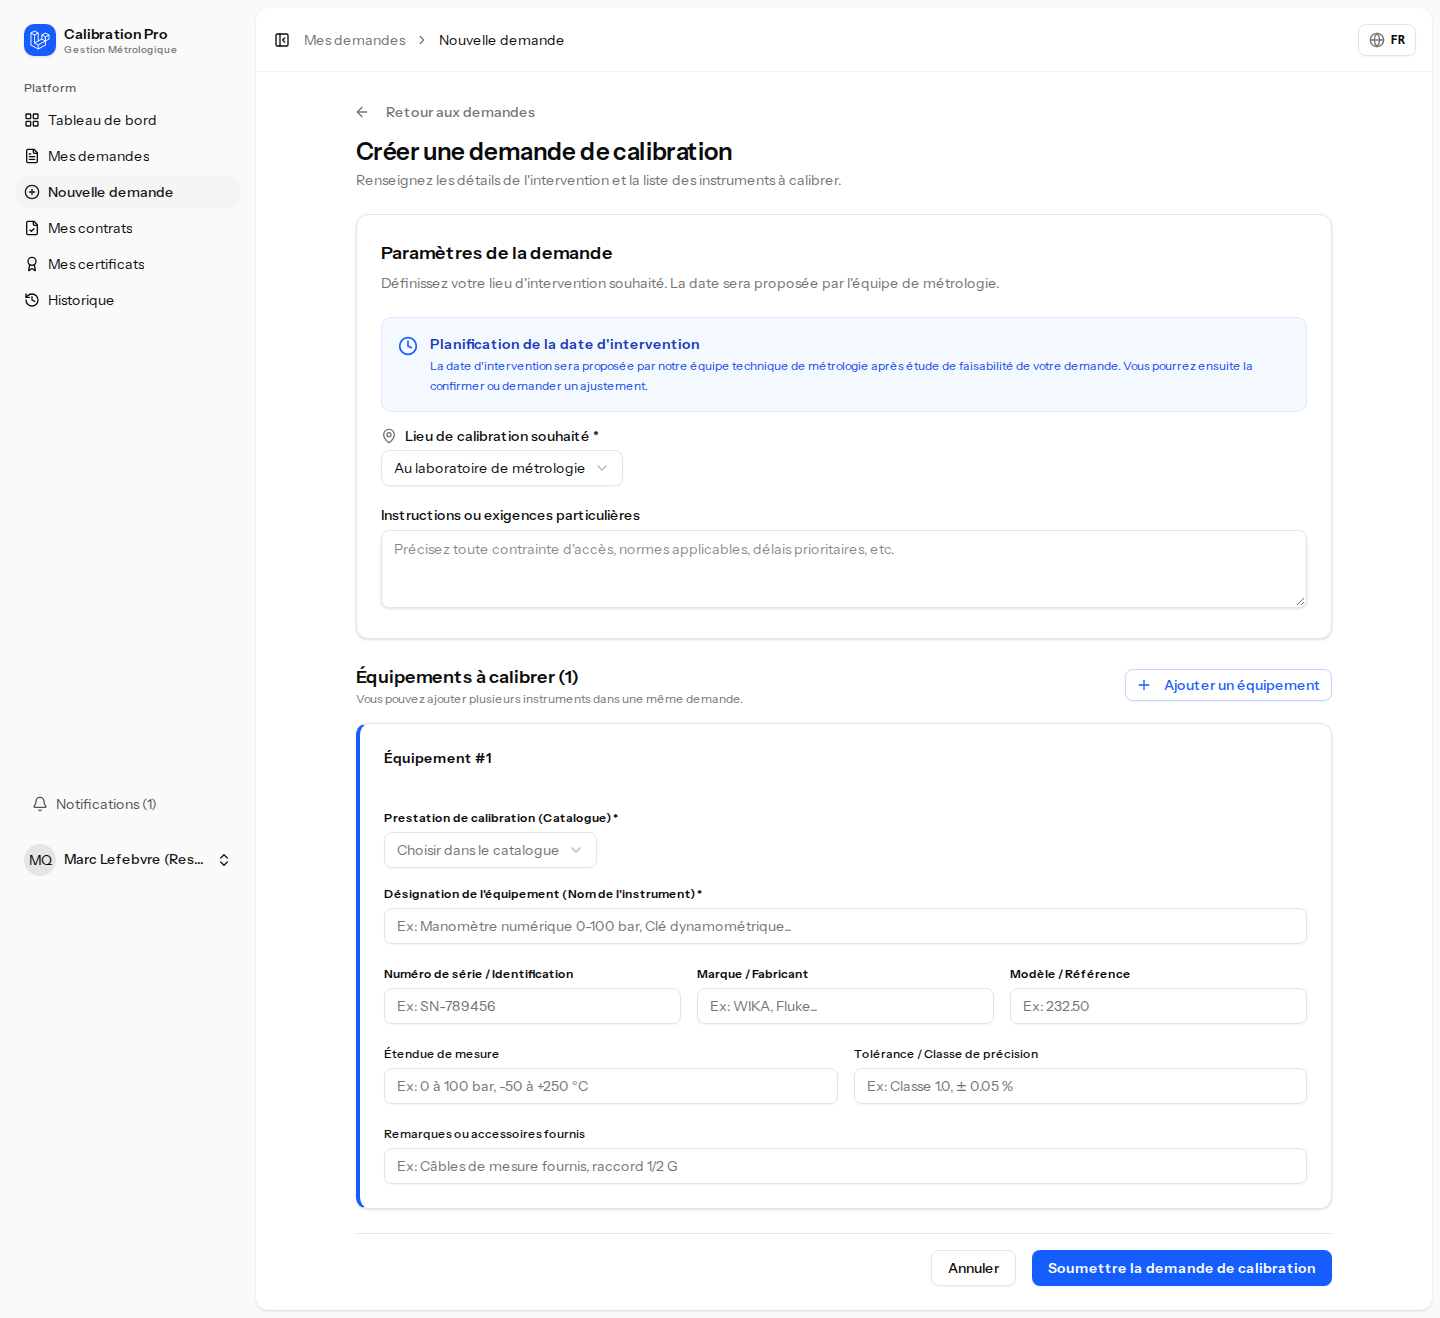
\includegraphics[width=0.9\linewidth]{figures/client-create.png}
  \end{LTR}
  \caption{فضاء الزبون : نموذج إدراج طلب معايرة متعدد المعدات}
  \label{fig:ui-client-create}
\end{figure}

\begin{figure}[H]
  \centering
  \begin{LTR}
  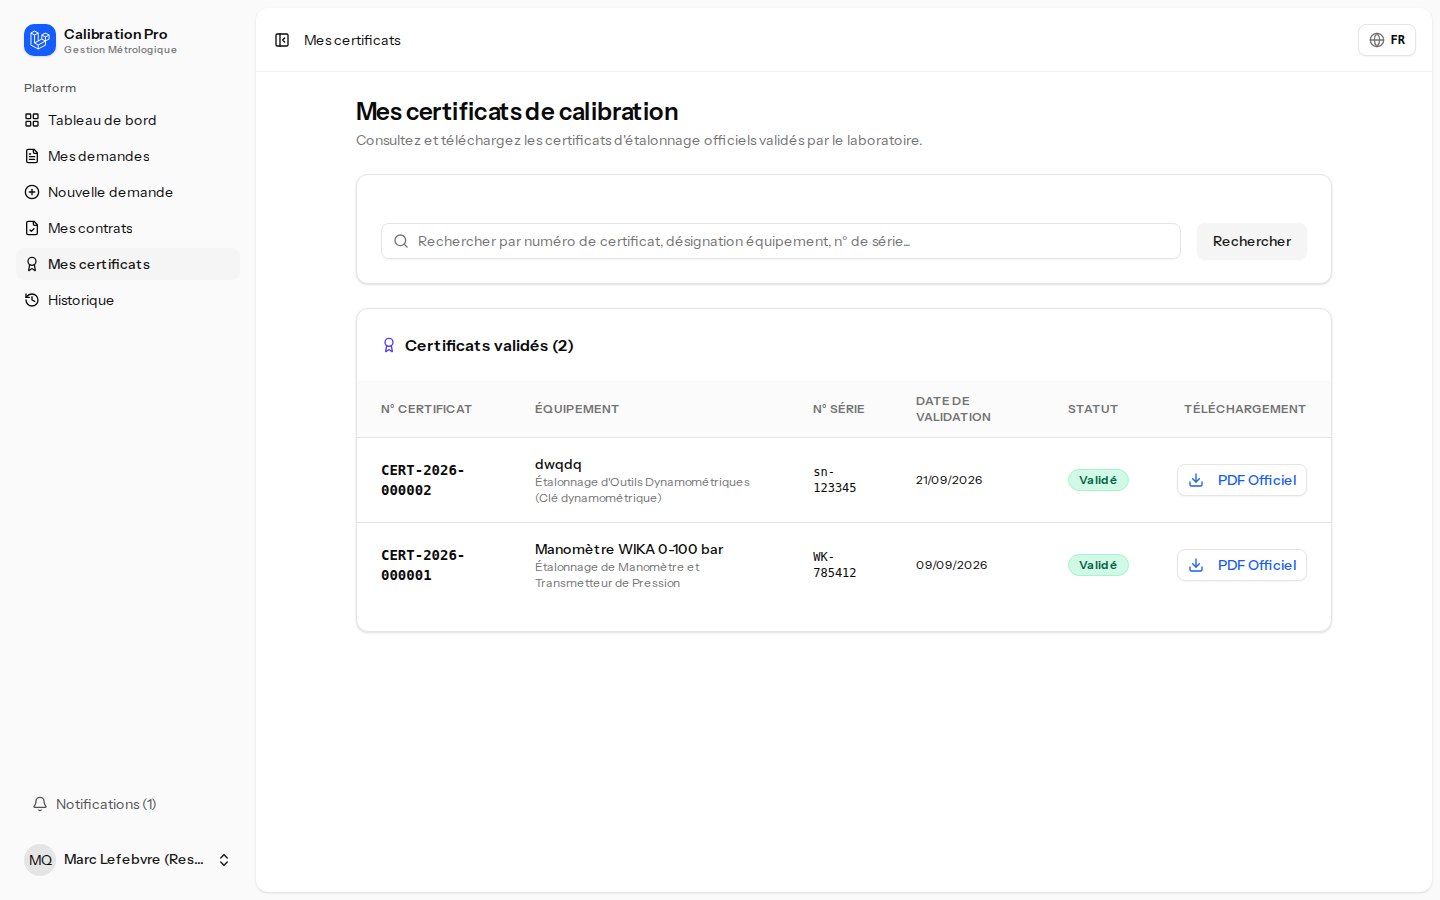
\includegraphics[width=0.9\linewidth]{figures/client-certificates.png}
  \end{LTR}
  \caption{فضاء الزبون : تحميل شهادات المعايرة المعتمدة}
  \label{fig:ui-client-certificates}
\end{figure}

\subsection{فضاء المصلحة التجارية}
يعالج المكلف التجاري الطلبات الواردة، فيطابق كل جهاز مع خدمة المعايرة المناسبة في الدليل، ويصدر الفاتورة التقديرية آلياً (HT + TVA 19\% = TTC)، قبل تحويل الملف إلى مسؤول المترولوجيا.

\begin{figure}[H]
  \centering
  \begin{LTR}
  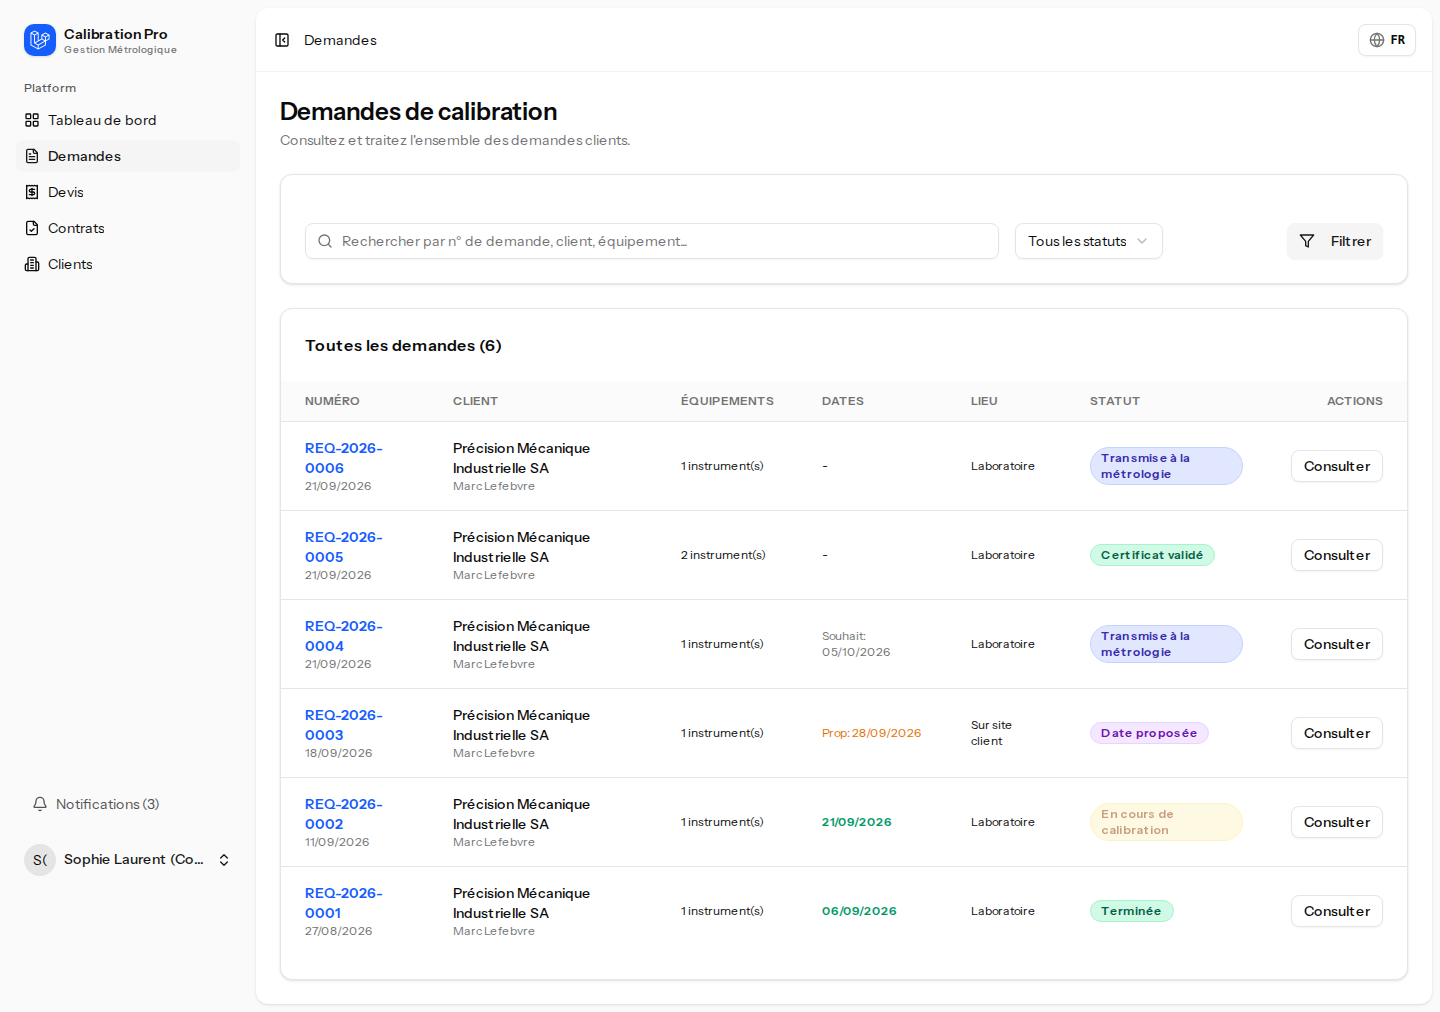
\includegraphics[width=0.9\linewidth]{figures/commercial-requests.png}
  \end{LTR}
  \caption{فضاء المصلحة التجارية : قائمة الطلبات الواردة وإصدار الفواتير التقديرية}
  \label{fig:ui-commercial-requests}
\end{figure}

\begin{figure}[H]
  \centering
  \begin{LTR}
  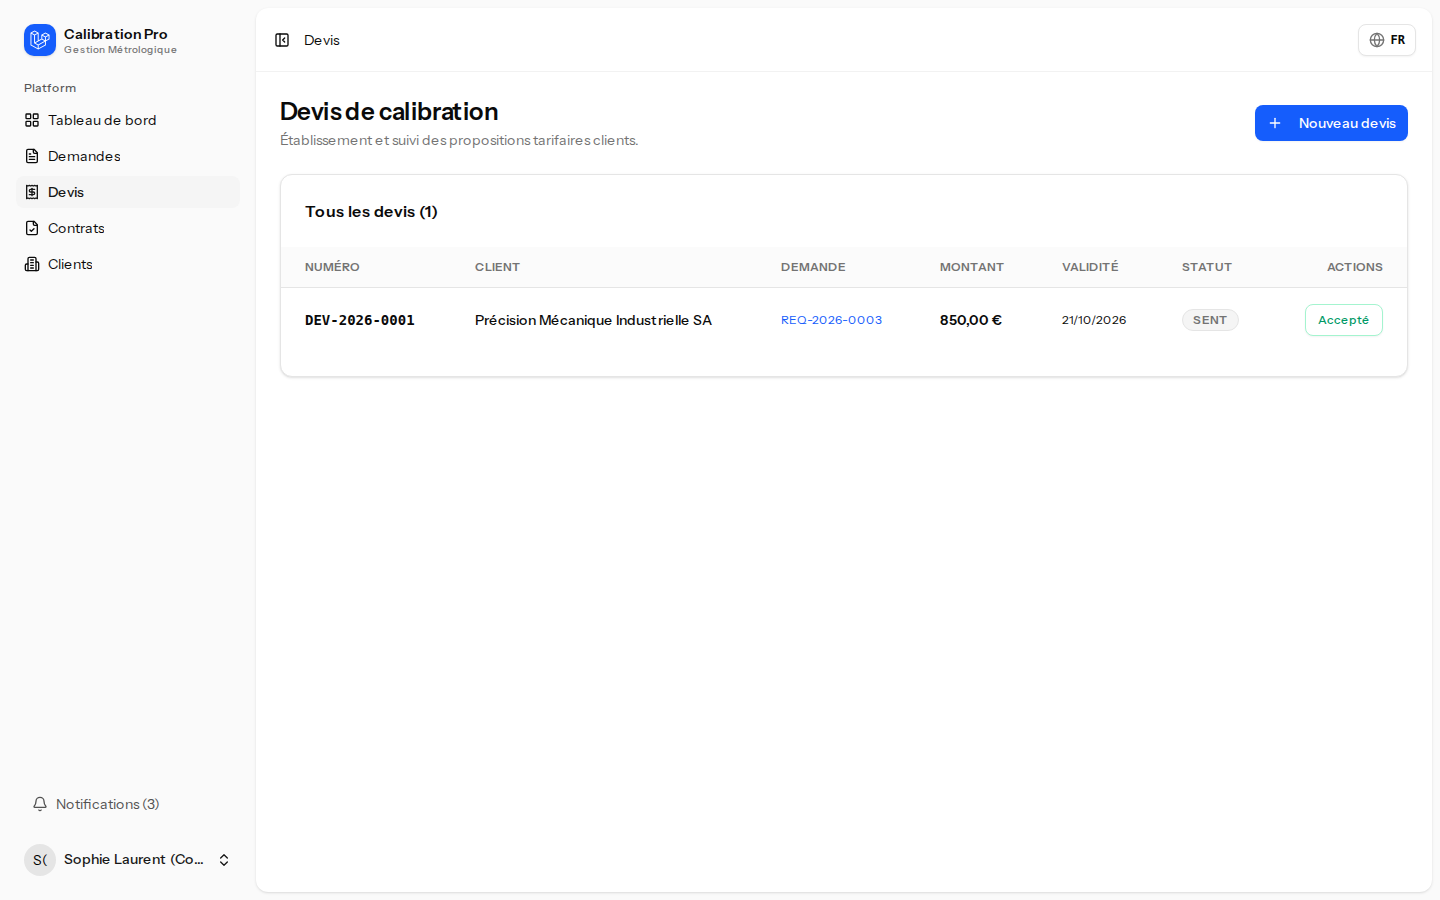
\includegraphics[width=0.9\linewidth]{figures/commercial-quotations.png}
  \end{LTR}
  \caption{فضاء المصلحة التجارية : إدارة الفواتير والمتابعة التعاقدية}
  \label{fig:ui-commercial-quotations}
\end{figure}

\subsection{لوحة تحكم مسؤول المترولوجيا}
تعتبر مركز القيادة الفني للمخبر، وتوفر:
\begin{itemize}
  \item إحصائيات بصرية شاملة عن توزيع الطلبات حسب الحالات والمجالات.
  \item أداة ذكية لتوزيع العمليات على التقنيين بحسب تخصصهم وعبء عملهم.
  \item واجهة تدقيق تقارير المعايرة مع إمكانية القبول أو طلب التعديل المعلل.
  \item نظام توقيع واعتماد الشهادات الرسمية وإغلاقها نهائياً.
\end{itemize}

\begin{figure}[H]
  \centering
  \begin{LTR}
  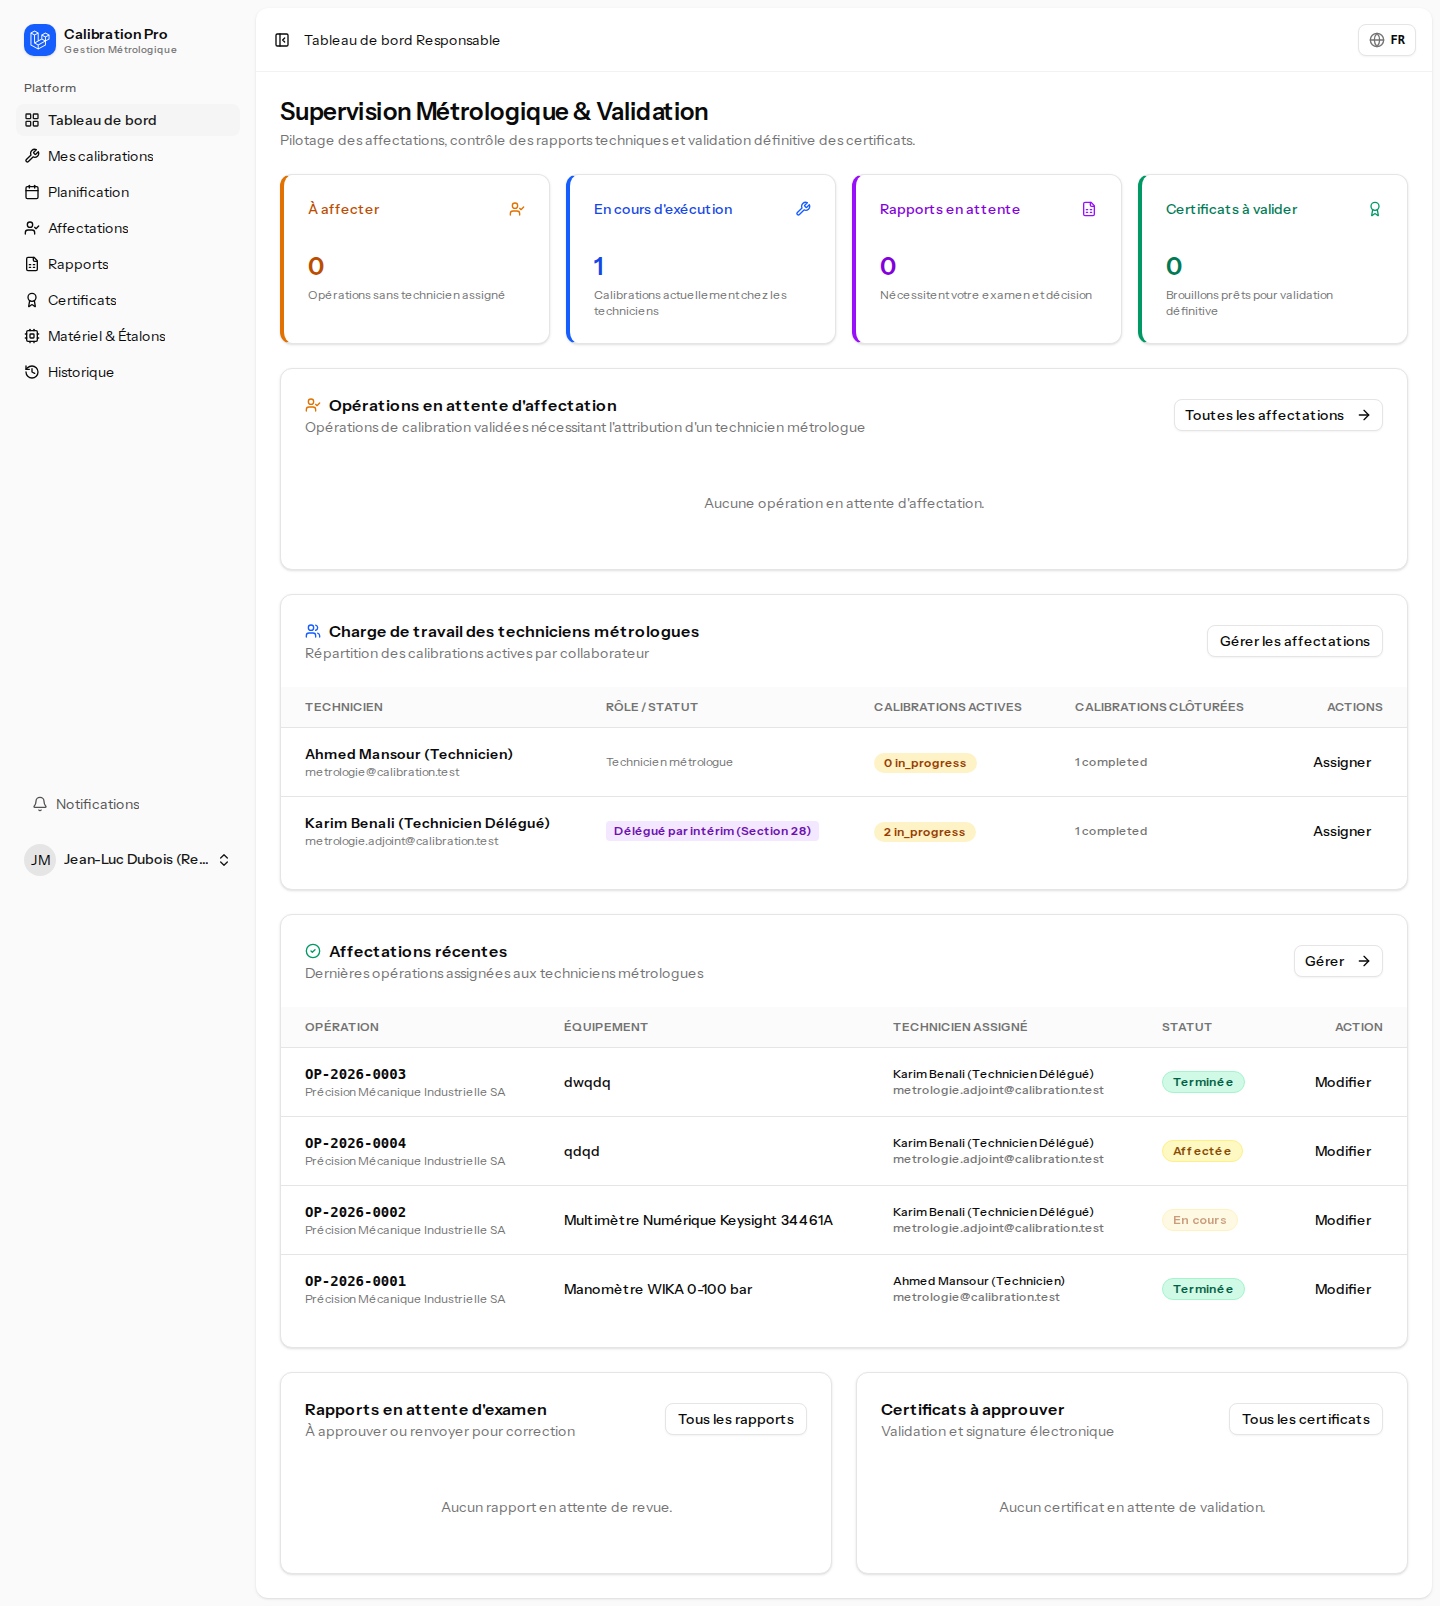
\includegraphics[width=0.9\linewidth]{figures/manager-dashboard.png}
  \end{LTR}
  \caption{لوحة تحكم مسؤول المترولوجيا : لوحة القيادة الفنية}
  \label{fig:ui-manager-dashboard}
\end{figure}

\begin{figure}[H]
  \centering
  \begin{LTR}
  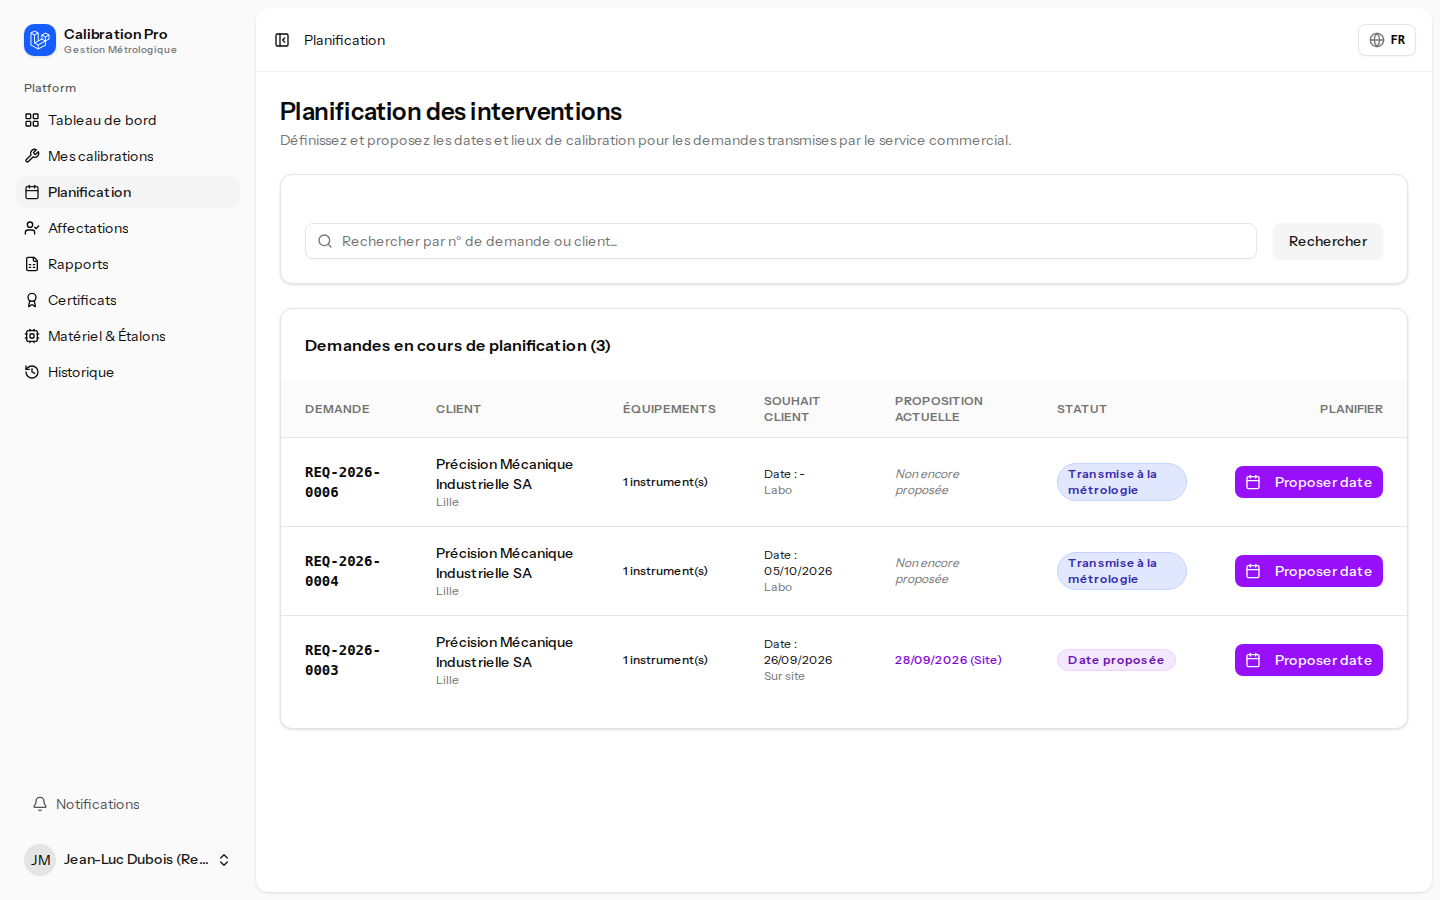
\includegraphics[width=0.9\linewidth]{figures/manager-scheduling.png}
  \end{LTR}
  \caption{مسؤول المترولوجيا : اقتراح مواعيد وأماكن المعايرة}
  \label{fig:ui-manager-scheduling}
\end{figure}

\begin{figure}[H]
  \centering
  \begin{LTR}
  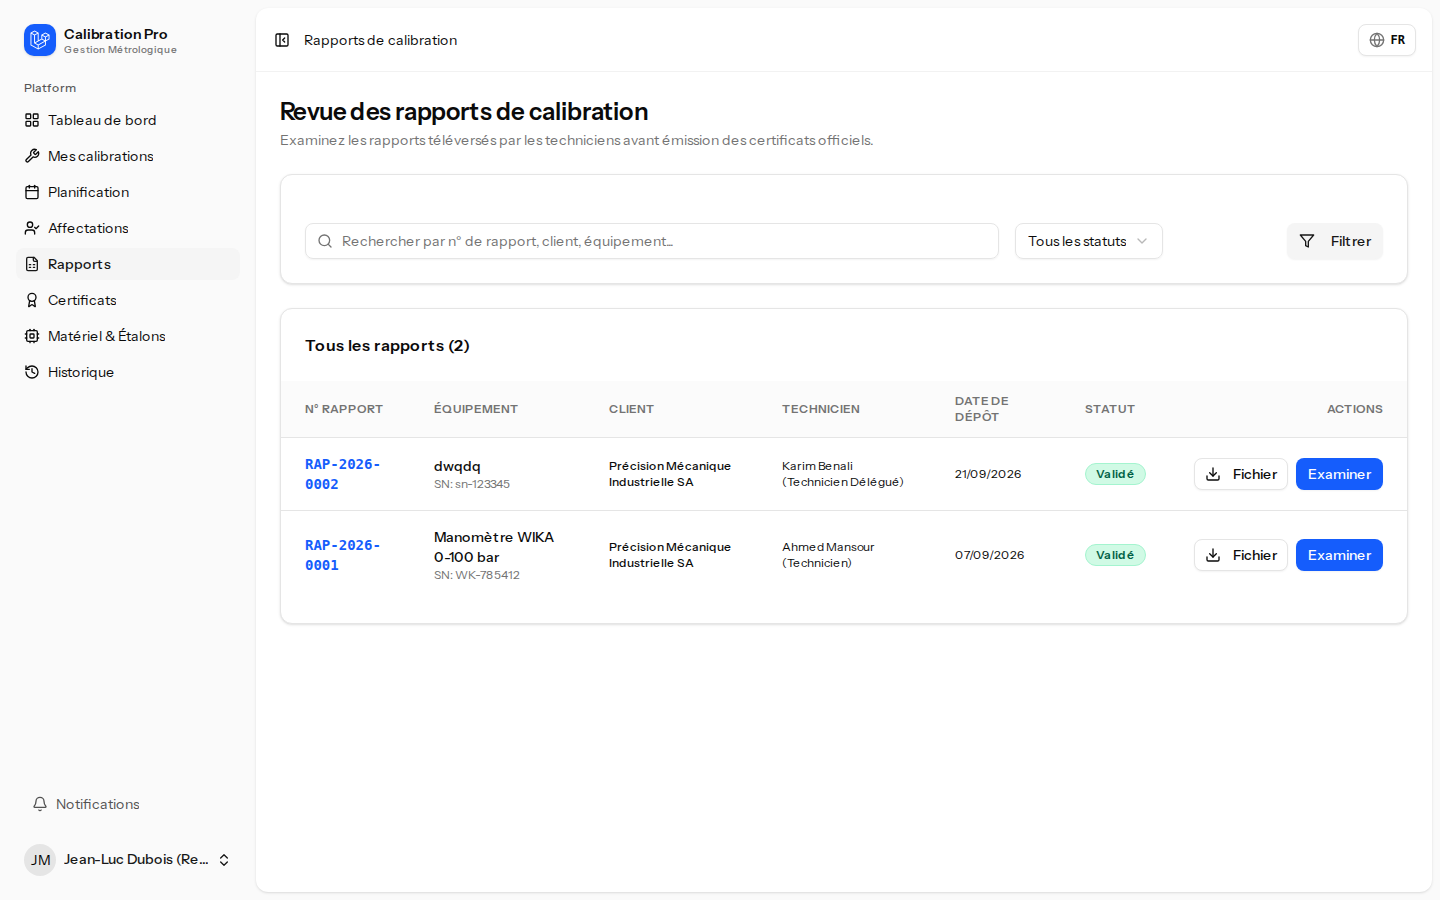
\includegraphics[width=0.9\linewidth]{figures/manager-reports.png}
  \end{LTR}
  \caption{مسؤول المترولوجيا : المراجعة النوعية لتقارير المعايرة}
  \label{fig:ui-manager-reports}
\end{figure}

\begin{figure}[H]
  \centering
  \begin{LTR}
  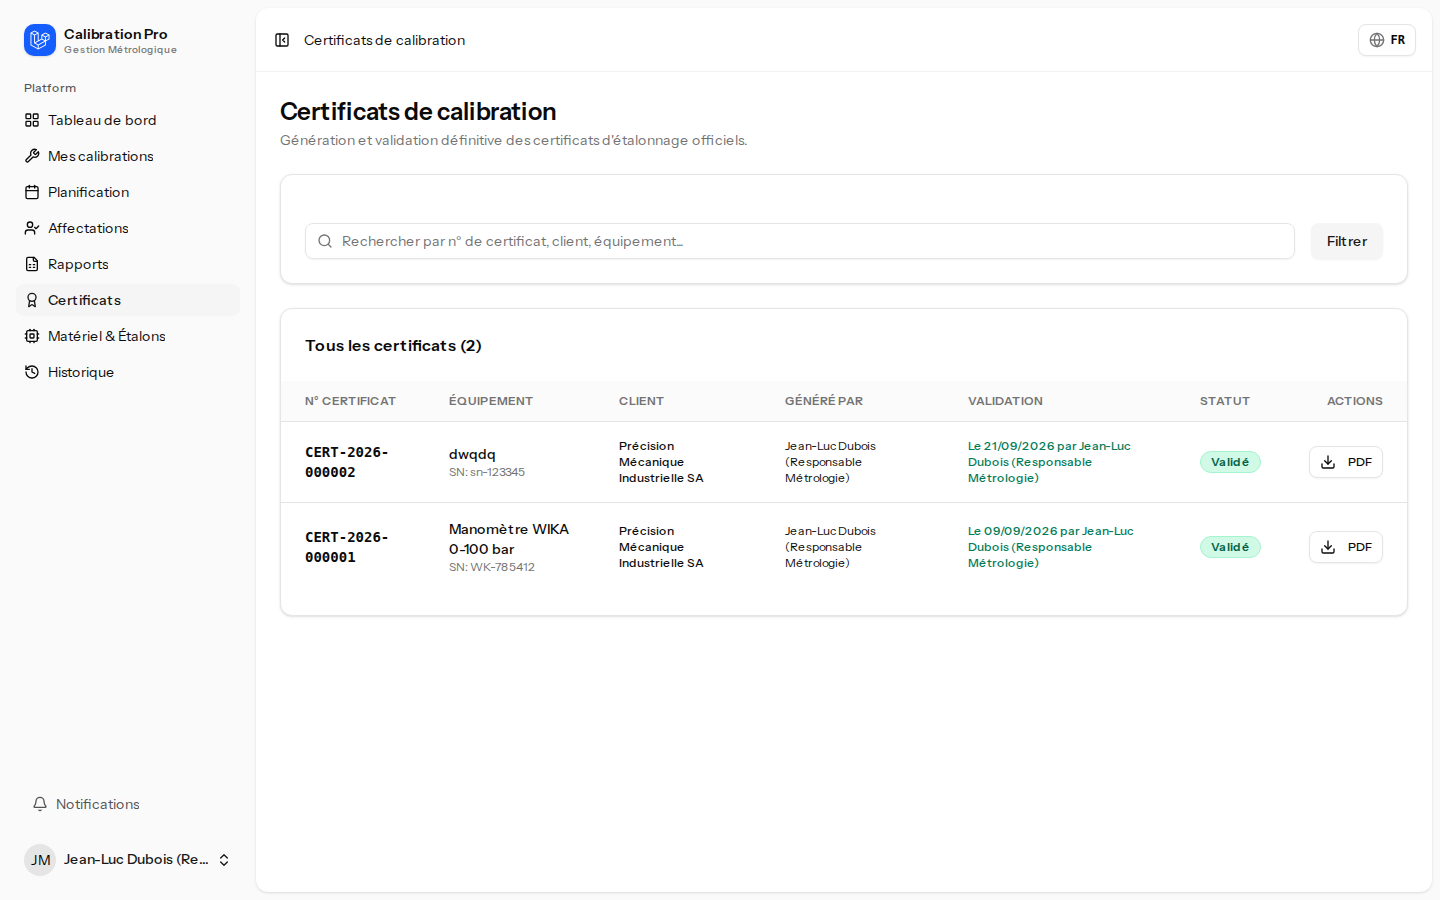
\includegraphics[width=0.9\linewidth]{figures/manager-certificates.png}
  \end{LTR}
  \caption{مسؤول المترولوجيا : اعتماد وتثبيت شهادات المعايرة الرسمية}
  \label{fig:ui-manager-certificates}
\end{figure}

\subsection{فضاء التقني المترولوجي}
شاشة مبسطة مخصصة لتقنيي المخابر، تعرض المهام الموكلة، وتتحقق من مطابقة الأجهزة العيارية المستعملة، وتوفر نموذجاً لرفع تقرير النتائج النهائي بصيغة PDF.

\begin{figure}[H]
  \centering
  \begin{LTR}
  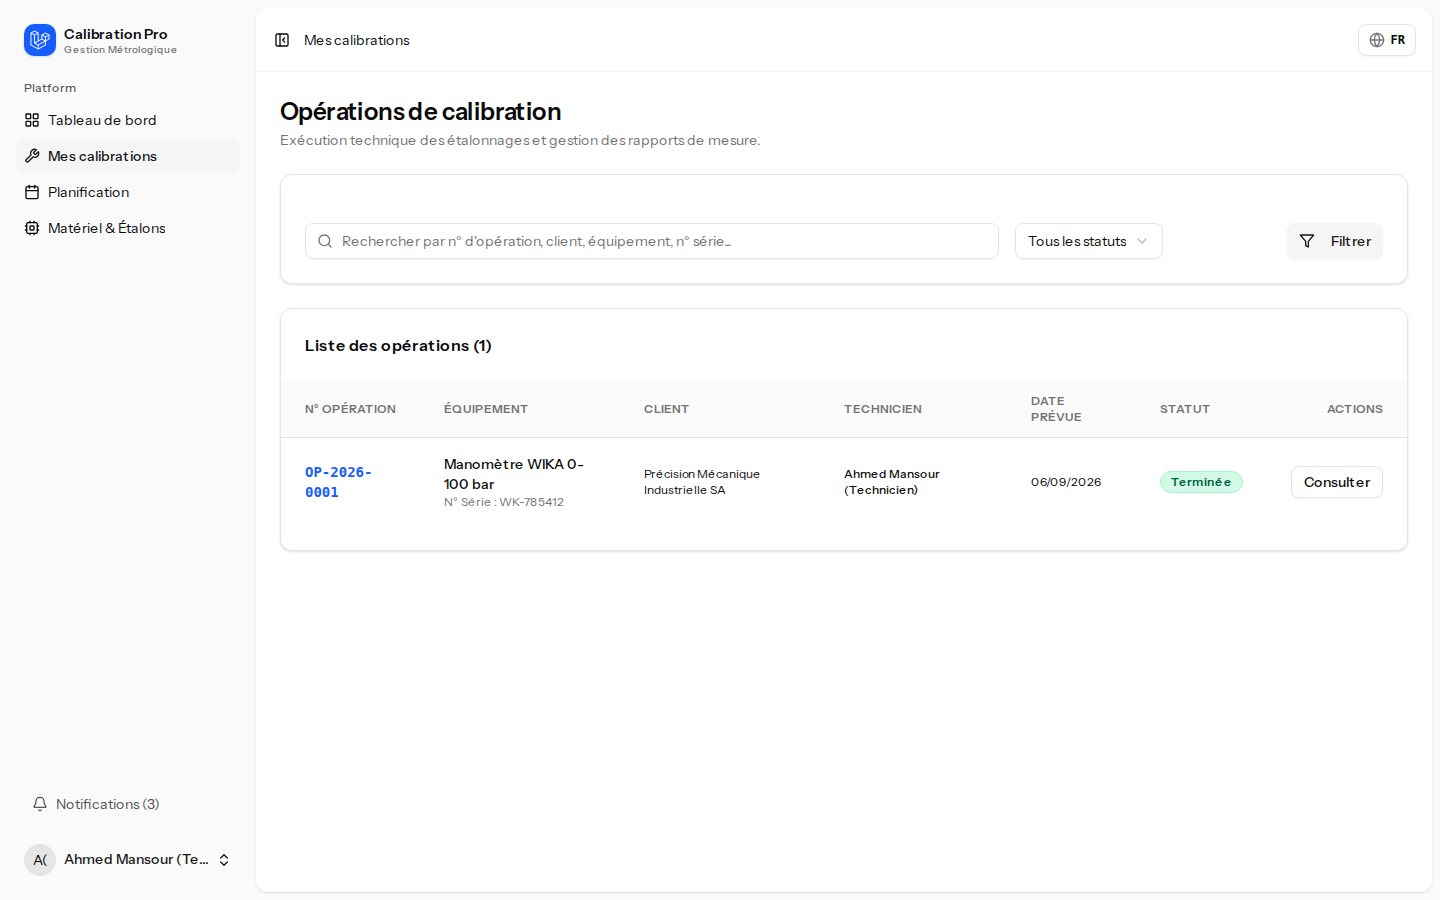
\includegraphics[width=0.9\linewidth]{figures/metrology-operations.png}
  \end{LTR}
  \caption{فضاء التقني المترولوجي : المهام الموكلة وتنفيذ المعايرة}
  \label{fig:ui-metrology-operations}
\end{figure}

\begin{figure}[H]
  \centering
  \begin{LTR}
  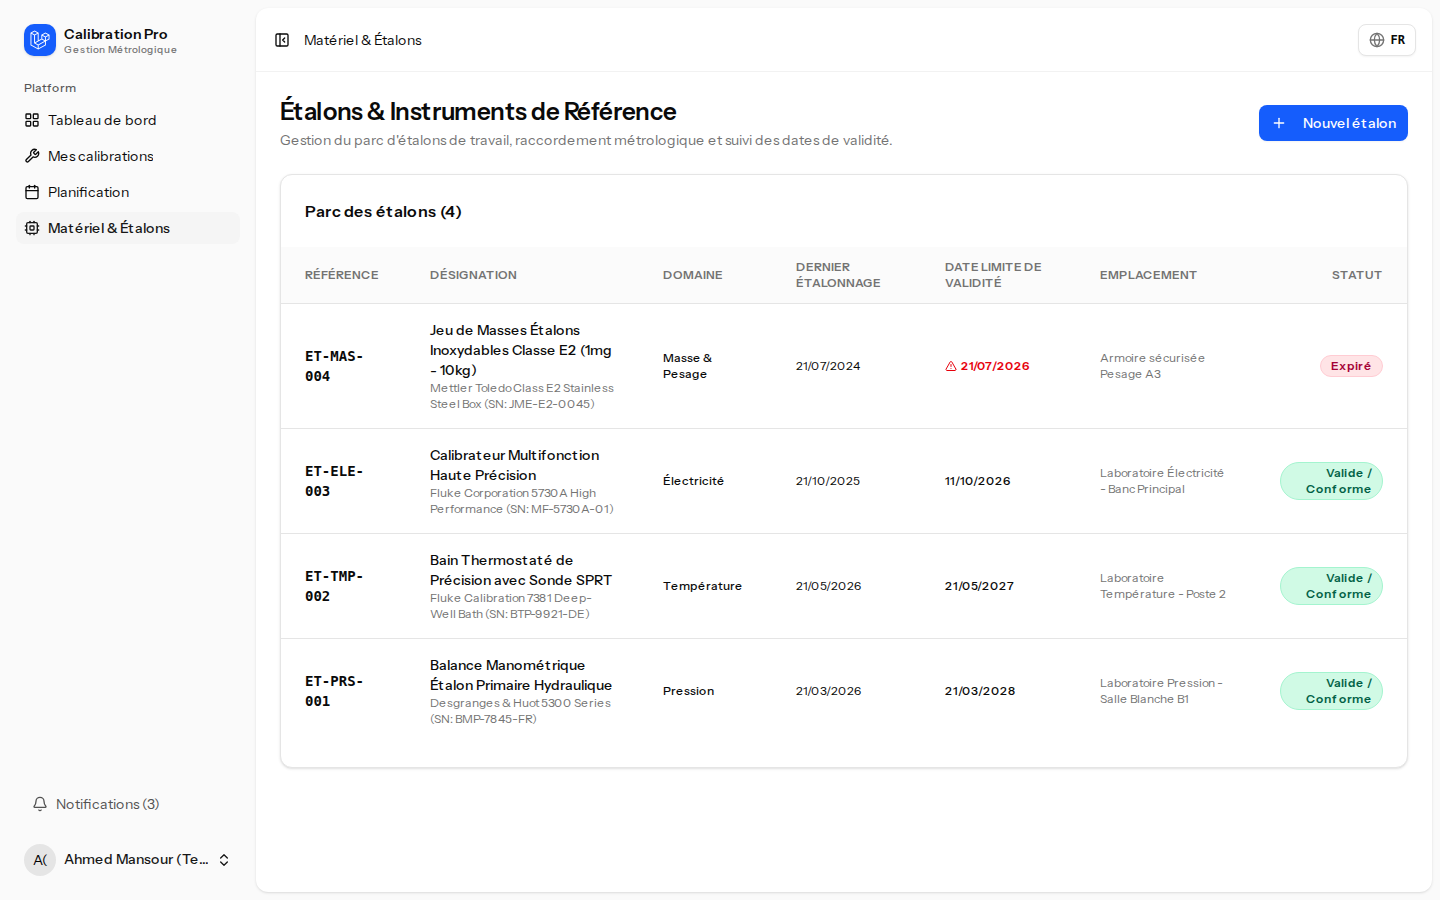
\includegraphics[width=0.9\linewidth]{figures/metrology-materials.png}
  \end{LTR}
  \caption{المترولوجيا : متابعة العتاد المرجعي وصيانته}
  \label{fig:ui-metrology-materials}
\end{figure}

\subsection{فضاء مسؤول النظام}
يمكّن مسؤول النظام من جرد حسابات المستخدمين وتدوير الرتب، وضبط دليل الخدمات والطاقات، والاطلاع على سجلات التدقيق الأمني والأرشيف الملتزم بشروط الحفظ.

\begin{figure}[H]
  \centering
  \begin{LTR}
  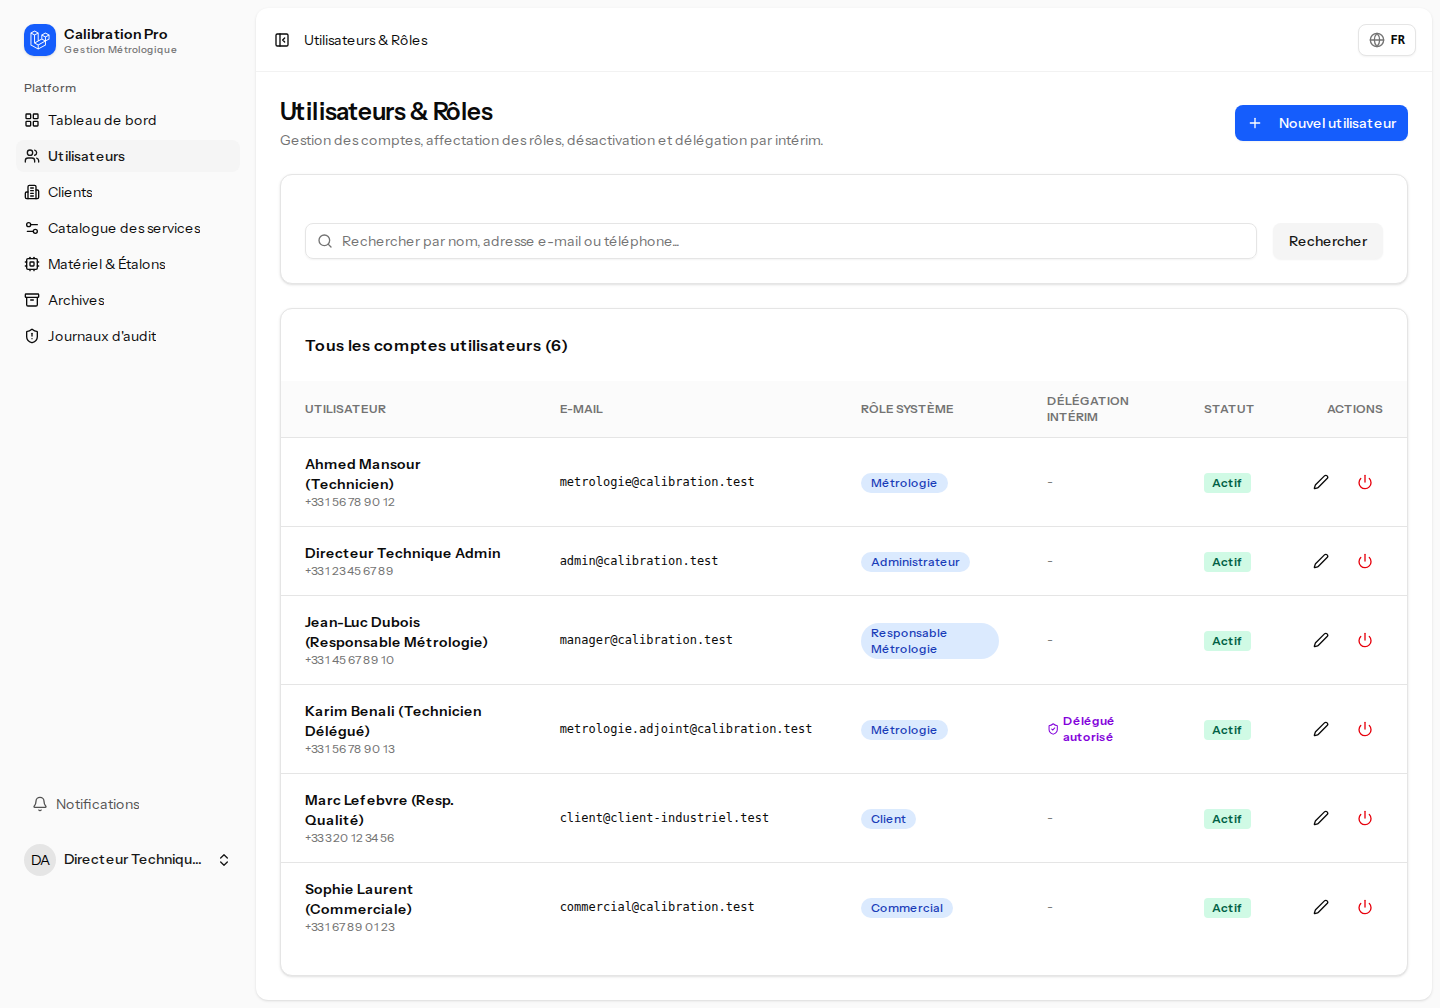
\includegraphics[width=0.9\linewidth]{figures/admin-users.png}
  \end{LTR}
  \caption{فضاء مسؤول النظام : إدارة حسابات المستخدمين والرتب}
  \label{fig:ui-admin-users}
\end{figure}

\begin{figure}[H]
  \centering
  \begin{LTR}
  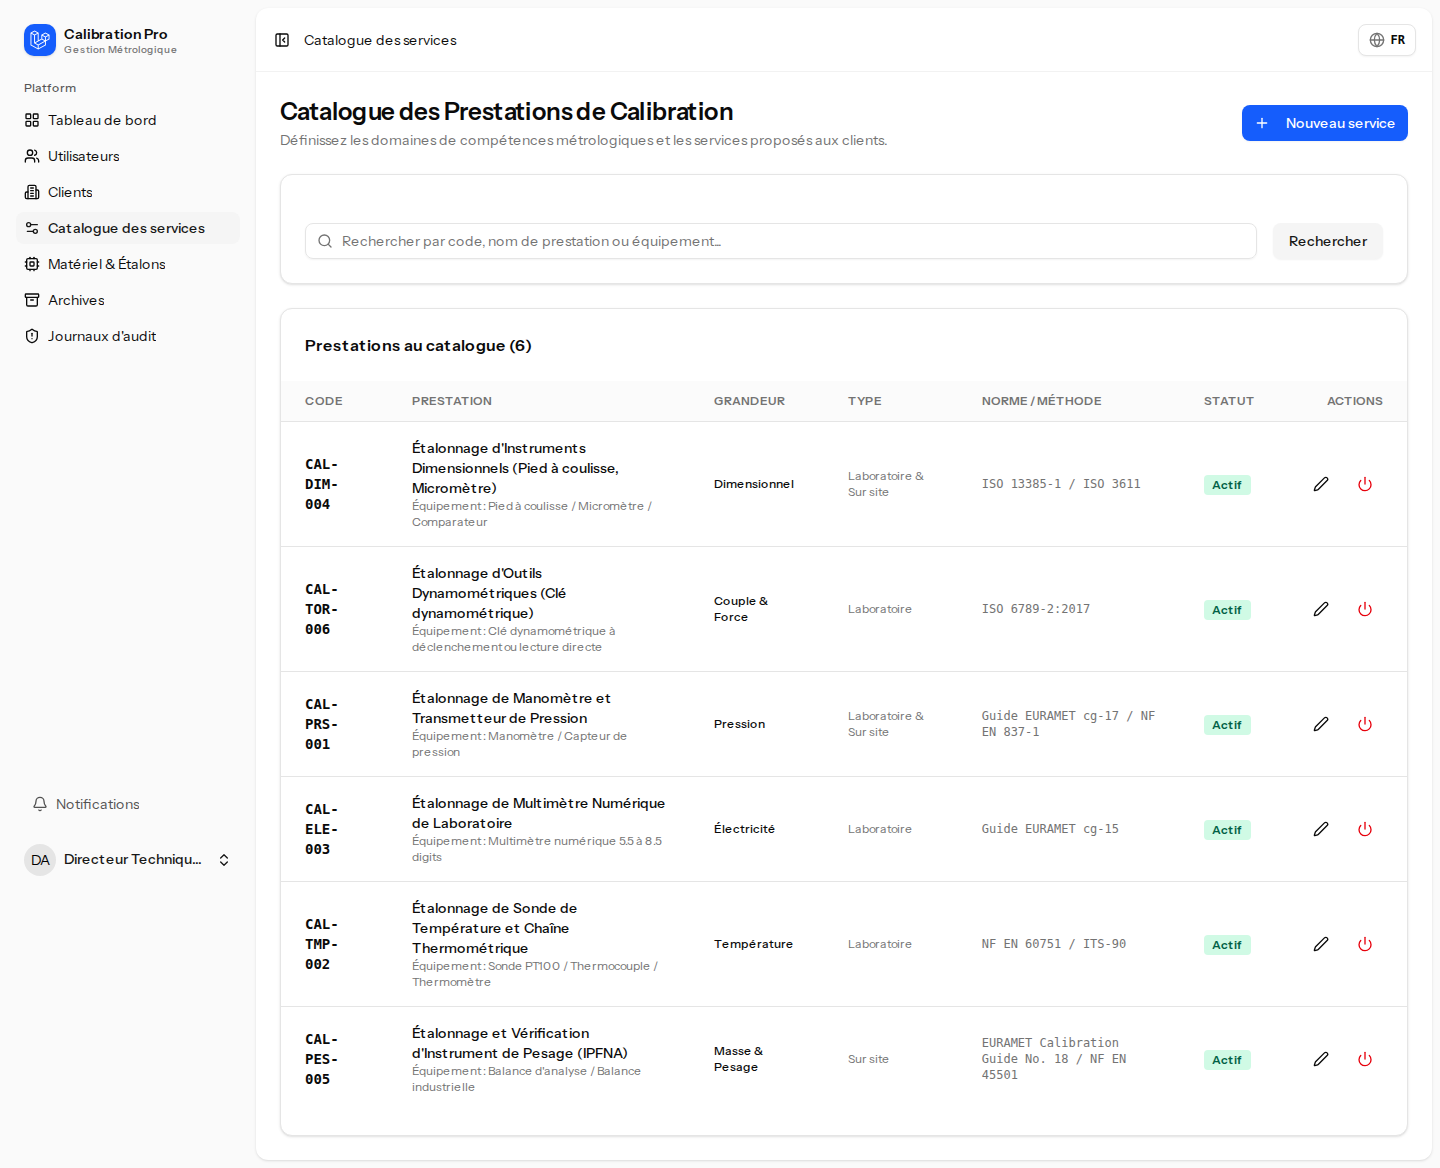
\includegraphics[width=0.9\linewidth]{figures/admin-services.png}
  \end{LTR}
  \caption{فضاء مسؤول النظام : ضبط دليل الخدمات المترولوجية}
  \label{fig:ui-admin-services}
\end{figure}

\begin{figure}[H]
  \centering
  \begin{LTR}
  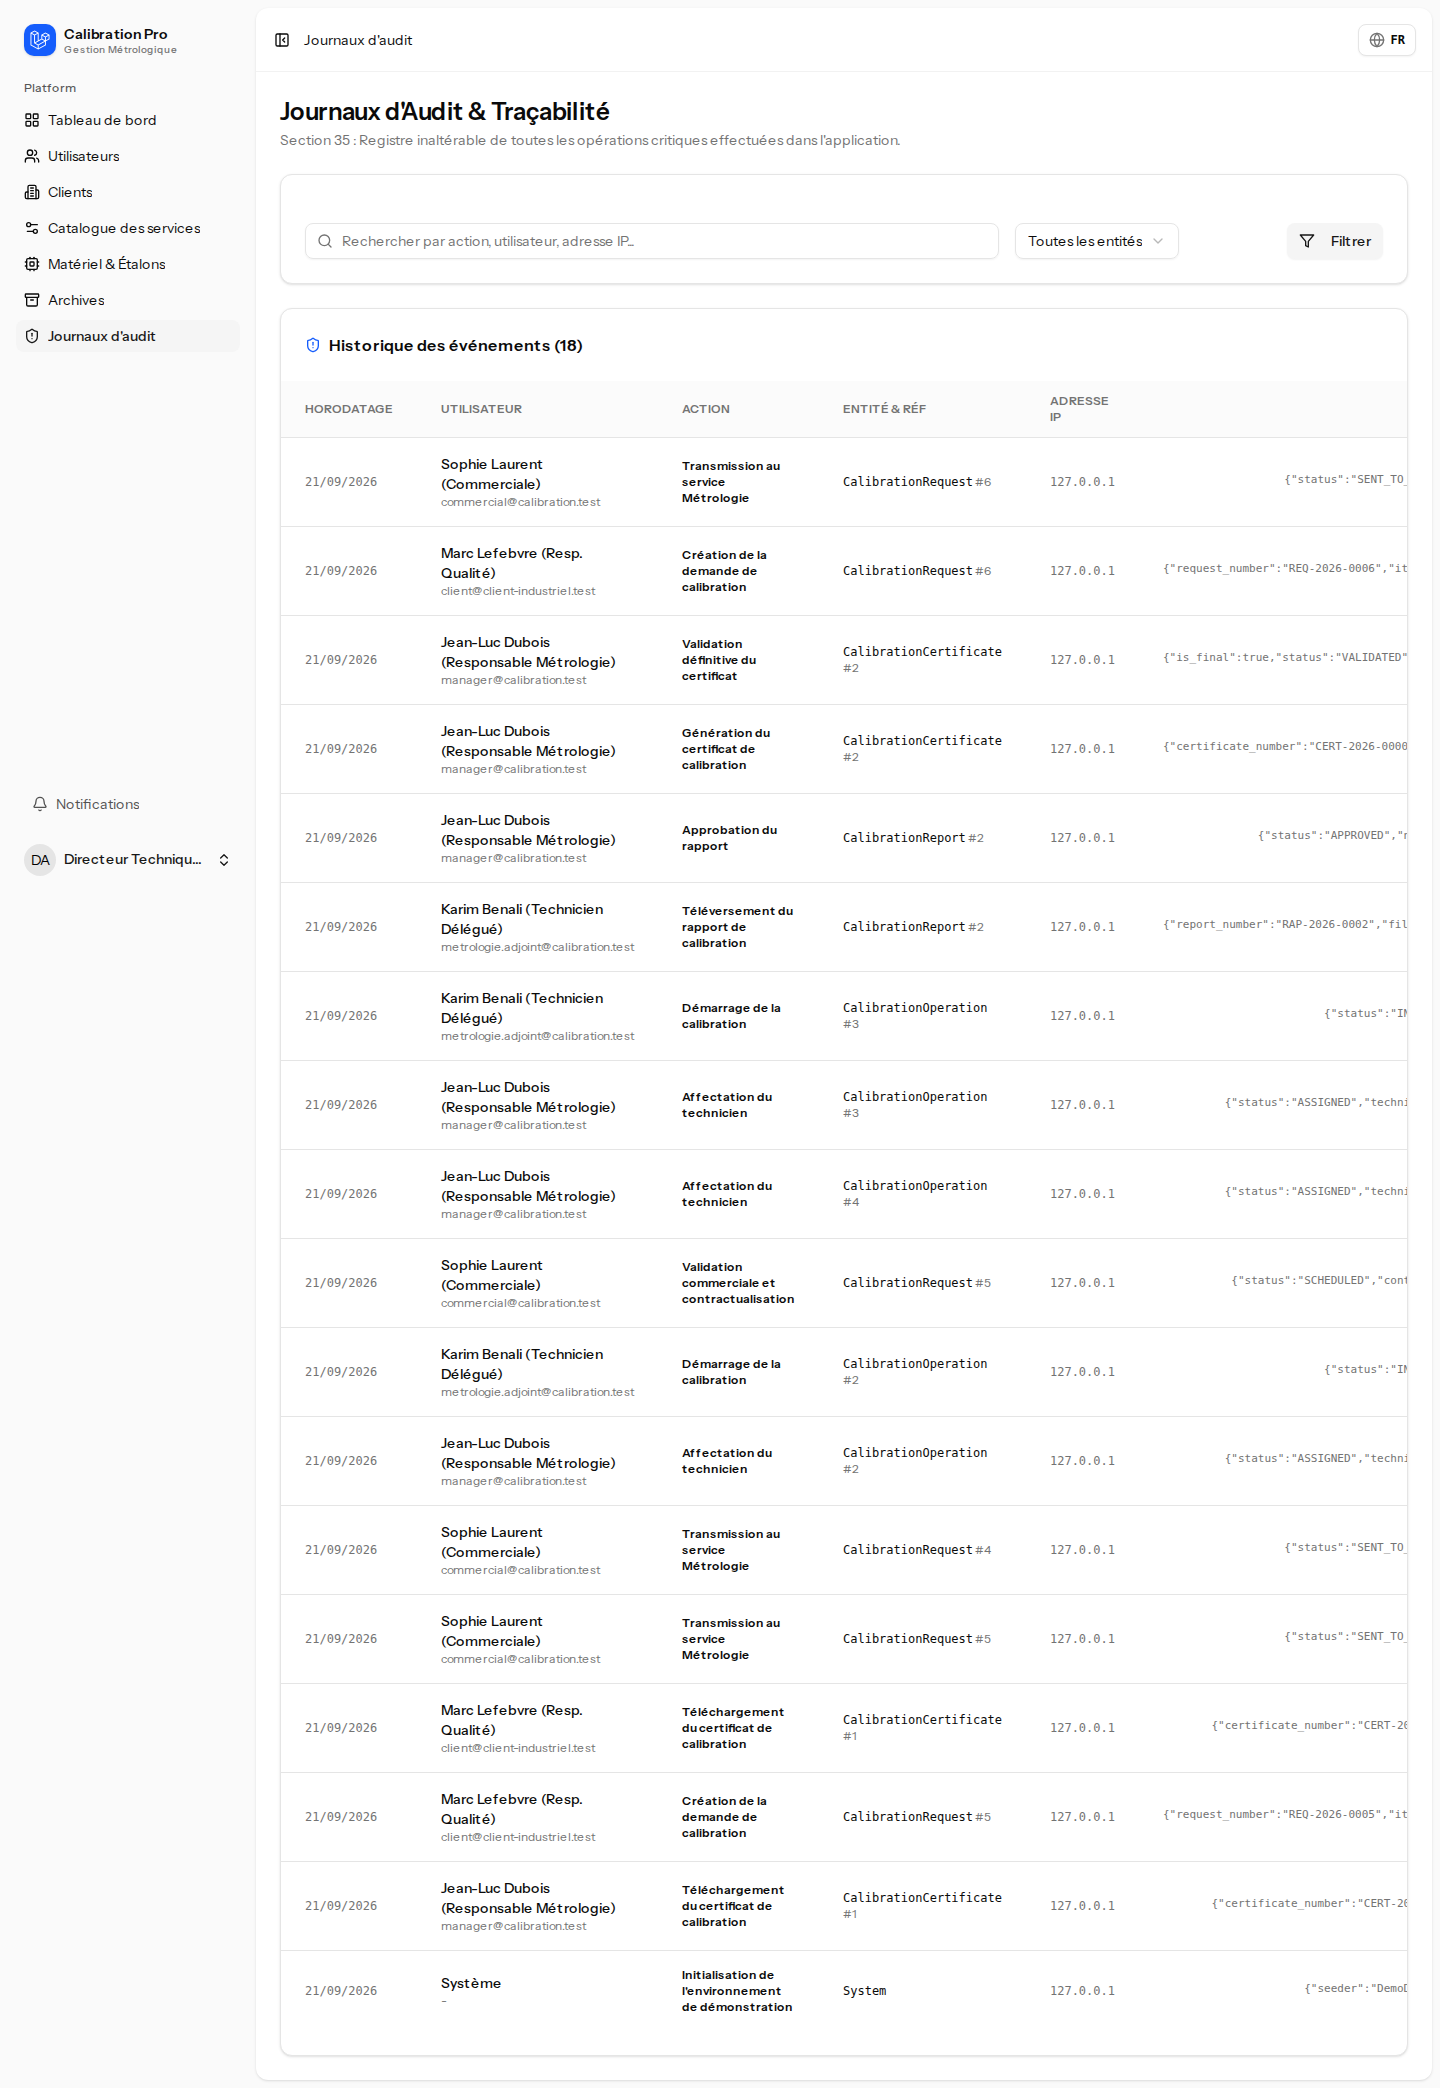
\includegraphics[width=0.9\linewidth]{figures/admin-audit.png}
  \end{LTR}
  \caption{فضاء مسؤول النظام : سجل التدقيق الأمني والتتبع الكامل}
  \label{fig:ui-admin-audit}
\end{figure}

\section{استراتيجية الاختبارات والتحقق الآلي}
\subsection{هرم الاختبارات}
لضمان أعلى معايير الجودة والموثوقية، قمنا بتنفيذ استراتيجية اختبارات آلية محكمة عبر مكتبة \textbf{Pest PHP} :

\begin{figure}[H]
  \centering
  \begin{LTR}
  \begin{tikzpicture}[>=Stealth,
    layer/.style={align=center, rounded corners=3pt, line width=0.8pt, minimum height=0.9cm, font=\footnotesize\bfseries},
    e2e/.style={layer, draw=red!70!black, fill=red!10, text width=2.2cm, minimum width=2.4cm},
    integ/.style={layer, draw=orange!80!black, fill=orange!10, text width=4.6cm, minimum width=4.8cm},
    unit/.style={layer, draw=blue!70!black, fill=blue!10, text width=7.2cm, minimum width=7.2cm}
]
\node[e2e] (e2e) at (0,3.2) {Tests d'Acceptation \& E2E\\[1pt]\scriptsize Authentification, Isolation Tenant};
\node[integ] (integ) at (0,1.5) {Tests d'Int\'egration \& Workflow (Feature)\\[1pt]\scriptsize 67 tests pass\'es / 273 assertions};
\node[unit] (unit) at (0,0) {Tests Unitaires (Models, Policies, Helpers)\\[1pt]\scriptsize Validation Immutabilit\'e \& Piste d'Audit};

\draw[thick, color=gray!70] (-5,-0.6) -- (0,5.65) -- (5,-0.6) -- cycle;
\end{tikzpicture}
  \end{LTR}
  \caption{هرم الاختبارات الآلية ومستويات الفحص}
  \label{fig:testing-pyramid}
\end{figure}

\subsection{نتائج حزمة الاختبارات الآلية}
أثبتت النتائج نجاح جميع الاختبارات الـ 67 بنسبة 100\% محققة 273 توكيداً أمنياً ووظيفياً:

\begin{teststablear}{نتائج حزمة الاختبارات الآلية المؤتمتة (Pest PHP / PHPUnit)}
  \testrowar{المصادقة وأمن الجلسات}{8}{8}{100\% ناجح [OK]}
  \testrowar{عزل بيانات الزبائن (Multi-Tenants)}{7}{7}{100\% ناجح [OK]}
  \testrowar{طلبات متعددة المعدات}{9}{9}{100\% ناجح [OK]}
  \testrowar{التسعير التجاري والفواتير التقديرية}{6}{6}{100\% ناجح [OK]}
  \testrowar{التنسيق والمصادقة على المواعيد}{6}{6}{100\% ناجح [OK]}
  \testrowar{تعيين العمليات ورفع التقارير}{8}{8}{100\% ناجح [OK]}
  \testrowar{الرقابة النوعية وطلب التصحيح المعلل}{7}{7}{100\% ناجح [OK]}
  \testrowar{عدم قابلية تعديل الشهادات النهائية}{6}{6}{100\% ناجح [OK]}
  \testrowar{التفويض الرسمي في التوقيع وتتبعه}{5}{5}{100\% ناجح [OK]}
  \testrowar{كشف وحظر الأدوات العيارية المنتهية}{5}{5}{100\% ناجح [OK]}
\end{teststablear}

\subsection{سيناريوهات التحقق الوظيفي الحرجة}
يغطي الجدول التالي أبرز سيناريوهات الاختبار الوظيفي التي تحمي المهام المترولوجية الحرجة، مع النتيجة المحصل عليها:

\begin{teststablear}{مصفوفة سيناريوهات التحقق الوظيفي الحرجة}
  \testrowar{إنشاء طلب متعدد المعدات من الزبون}{1}{1}{ناجح [OK]}
  \testrowar{دراسة الطلب وربطه بخدمات الدليل}{1}{1}{ناجح [OK]}
  \testrowar{اقتراح تاريخ ومكان المعايرة والتحقق من قبول الزبون أو رفضه بتعليل}{1}{1}{ناجح [OK]}
  \testrowar{تعيين العملية للتقني ورفع تقرير المعايرة}{1}{1}{ناجح [OK]}
  \testrowar{طلب إعادة المعالجة (Rework) بتبرير إجباري}{1}{1}{ناجح [OK]}
  \testrowar{اعتماد التقرير وتوليد مسودة الشهادة}{1}{1}{ناجح [OK]}
  \testrowar{توقيع الشهادة في وضع التفويض المخول}{1}{1}{ناجح [OK]}
  \testrowar{منع أي تعديل على الشهادة النهائية (Immutability)}{1}{1}{ناجح [OK]}
  \testrowar{عزل بيانات الزبائن ورفض الوصول لبيانات الغير}{1}{1}{ناجح [OK]}
  \testrowar{تنبيه وحظر العتاد المرجعي المنتهية صلاحيته}{1}{1}{ناجح [OK]}
  \testrowar{تسجيل سجل التدقيق الكامل للمستخدم وعنوان IP}{1}{1}{ناجح [OK]}
\end{teststablear}

\subsection{واجهة تشغيل الاختبارات الآلية}
نُفذت الحزمة التجريبية عبر أمر \LR{\texttt{php artisan test}} فأظهرت النتيجة التالية:

\begin{figure}[H]
  \centering
  \begin{LTR}
  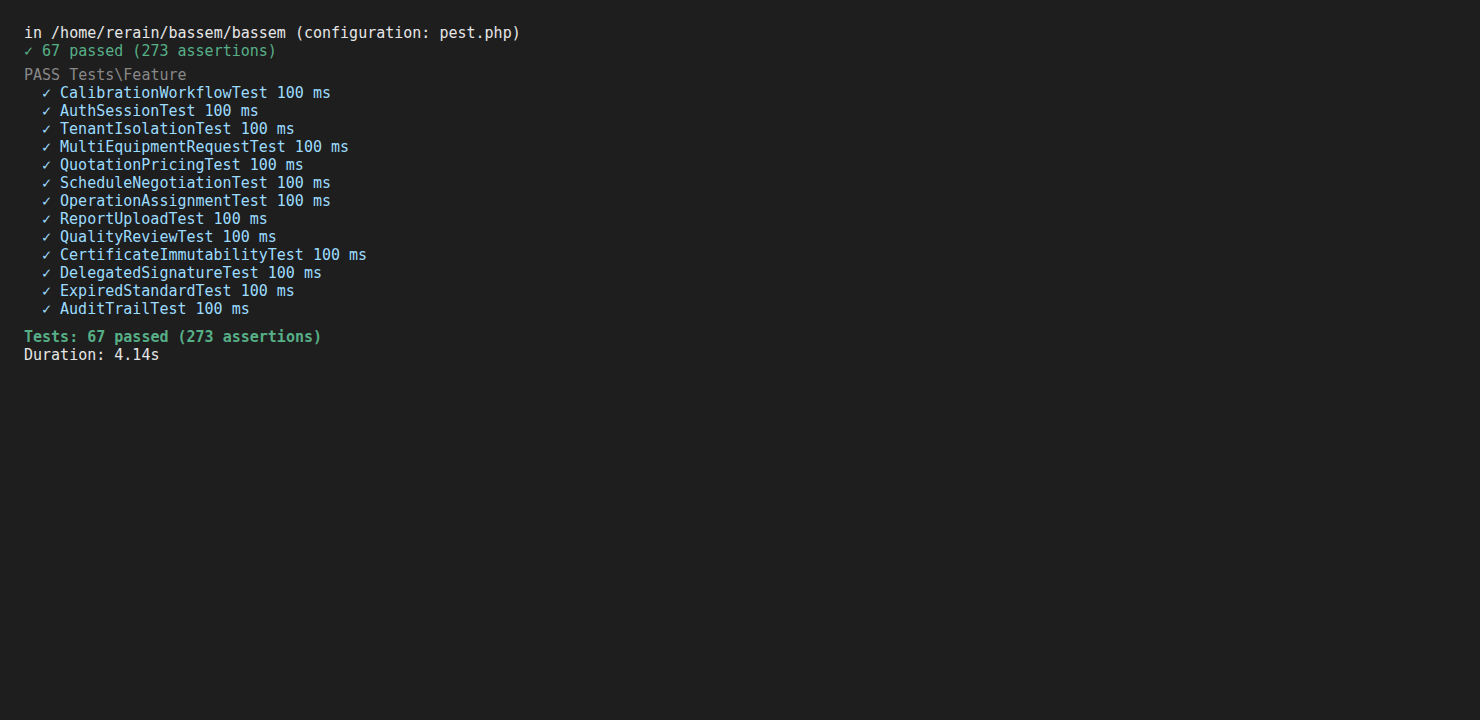
\includegraphics[width=0.85\linewidth]{figures/test-runner.png}
  \end{LTR}
  \caption{مخرجات تشغيل حزمة الاختبارات الآلية (67 اختباراً ناجحاً)}
  \label{fig:test-runner}
\end{figure}

\begin{LTR}
\begin{quote}
\ttfamily
   PASS  Tests\textbackslash Feature\textbackslash CalibrationWorkflowTest\\
  Tests:    67 passed (273 assertions)\\
  Duration: 4.13s
\end{quote}
\end{LTR}

\section*{خاتمة الفصل الرابع}
أثبت هذا الفصل نجاح التطبيق العملي للنظام وقدرته على تلبية المتطلبات المترولوجية الدقيقة بكفاءة وسرعة، مع تحقيق أعلى مستويات الأمان بفضل الاختبارات الآلية المحكمة.


%% ============================================================
%% الخاتمة العامة والآفاق المستقبلية
%% ============================================================
\chapter*{الخاتمة العامة والآفاق المستقبلية}
\addcontentsline{toc}{chapter}{الخاتمة العامة والآفاق المستقبلية}

\section*{حصيلة المشروع}
تناول هذا العمل تصميم وإنجاز تطبيق ويب متكامل ومخصص لتسيير ومتابعة عمليات معايرة معدات القياس والمترولوجيا الصناعية وفق معايير الجودة الدولية (ISO/IEC 17025) لصالح المخبر الوطني للمعايرة (LNEMI).

وقد مكننا هذا المشروع من تطبيق المفاهيم الحديثة لهندسة البرمجيات بالاعتماد على المنهجية الموحدة ولغة UML، وبناء منصة متينة تجمع بين قوة إطار العمل \textbf{Laravel 12}، وسلاسة مكتبة \textbf{React 19} عبر تقنية \textbf{Inertia.js}.

وقد تم تحقيق جميع الأهداف المسطرة بنجاح تام:
\begin{itemize}
  \item التخلص النهائي من السجلات الورقية وتشتت البيانات عبر توفير قاعدة بيانات مركزية متناسقة.
  \item تسريع معالجة الطلبات وإتاحة التنسيق الفوري بين الزبون والمخبر حول مواعيد التدخل.
  \item الحماية القانونية التامة لشهادات المعايرة بفرض قفل عدم قابلية التعديل (\texttt{is\_final = true}) فور المصادقة.
  \item القضاء على المخاطر المترولوجية بالحظر التلقائي لاستخدام الأجهزة العيارية المنتهية الصلاحية.
  \item إثبات وتوثيق كافة العمليات الحساسة عبر سجل تدقيق أمني غير قابل للحذف.
\end{itemize}

\section*{الصعوبات والقيود}
رغم نجاح الإنجاز، سُجلت بعض الصعوبات والقيود التي واجهتنا أثناء هذا العمل ويتعين ذكرها بشفافية:
\begin{itemize}
  \item \textbf{تعقيد مجال المترولوجيا :} اقتضى استيعاب المفاهيم الفيزيائية والمعيارية (الارتياب في القياس، نطاقات الصلاحية، التسلسل المترولوجي) جهداً كبيراً لفهمها وصياغتها برمجياً بشكل صحيح، خاصة قواعد \LR{\texttt{ISO/IEC 17025}} المتعلقة بالشهادات والعقود.
  \item \textbf{إدارة الحالة المتشعبة :} التحكم في التتابع الكامل للحالات (طلب $\rightarrow$ فاتورة $\rightarrow$ جدولة $\rightarrow$ معايرة $\rightarrow$ شهادة) مع كل الفروقات والتفرعات يتطلب صلابة في التصميم واختبارات تغطية واسعة، وتأخر بعض الوظائف الثانوية إلى الإصدارات اللاحقة.
  \item \textbf{الحاجز اللغوي والبيئة :} كتابة كل الوثائق والمخرجات بالعربية مع الاحتفاظ بالدقة التقنية للمصطلحات الإنجليزية والفرنسية فرض عمل توثيقي إضافي، كما أن غياب تأطير تقني دائم في بعض مراحل التطوير زاد من مدة التجريب.
  \item \textbf{قيود الأداء على العتاد المتواضع :} توظيف التشفير والتدقيق على كل عملية حساسة ينعكس على استجابة النظام في بيئات التطوير المحلية، وهو ما تمت معالجته عبر تحسين الاستعلامات والفهرسة، مع إمكانية التحسين مستقبلاً بالوسائط التقنية.
\end{itemize}
وبذلك تبقى هذه الصعوبات إطاراً دافعاً لتحسينات قادمة أكثر من كونها حدوداً فنية نهائية.

\section*{الآفاق المستقبلية}
لتعزيز قدرات هذا النظام مستقبلاً، نقترح الآفاق التطويرية التالية:
\begin{enumerate}
  \item \textbf{التوقيع الرقمي المعتمد (PKI) :} إدماج تقنيات التوقيع الإلكتروني المشفر بمفاتيح التشفير العامة داخل ملفات PDF للشهادات وفق معايير الهيئات الرسمية.
  \item \textbf{تطبيق متنقل دون اتصال (PWA Offline) :} تطوير تطبيق هجين يسمح للتقنيين في المواقع الصناعية البعيدة بتسجيل قياساتهم دون الحاجة لشبكة إنترنت، مع المزامنة الآلية فور توفر الاتصال.
  \item \textbf{الربط الذكي مع أجهزة القياس (IoT) :} ربط منصات القياس الحديثة مباشرة مع النظام لسحب قراءات الارتياب آلياً دون أي تدخل بشري في كتابة النتائج.
  \item \textbf{بطاقات التعريف الذكية (QR Code) :} تثبيت ملصقات تحمل رمز الاستجابة السريعة على كل معدة تمت معايرتها، ليتمكن مدققو الجودة من التحقق من صحة الشهادة بمجرد مسح الرمز بالهاتف.
\end{enumerate}


%% ============================================================
%% قائمة المراجع والمصادر
%% ============================================================
\chapter*{قائمة المراجع والمصادر (Bibliographie)}
\addcontentsline{toc}{chapter}{قائمة المراجع والمصادر}

\begin{thebibliography}{12}

\bibitem{iso17025}
\textbf{ISO/IEC 17025:2017} : \textit{Exigences g\'en\'erales concernant la comp\'etence des laboratoires d'\'etalonnage et d'essais}. Organisation Internationale de Normalisation, Gen\`eve, Suisse, 2017.

\bibitem{guide-insfp}
\textbf{INSFP Rahmania} : \textit{Guide m\'ethodologique de pr\'eparation du m\'emoire de fin de formation -- Option D\'eveloppeur Web et Mobile}. Institut National Sp\'ecialis\'e de la Formation Professionnelle Rahmania, Alger, Alg\'erie.

\bibitem{booch-uml}
\textbf{BOOCH, G., RUMBAUGH, J., JACOBSON, I}. \textit{The Unified Modeling Language User Guide} (2nd Edition). Addison-Wesley Professional, 2005.

\bibitem{laravel-docs}
\textbf{OTWELL, T.}. \textit{Laravel Documentation -- The PHP Framework for Web Artisans}. [en ligne]. \url{https://laravel.com/docs} [consult\'e le 15/09/2026].

\bibitem{inertia-docs}
\textbf{REININK, J.}. \textit{Inertia.js -- The Modern Monolith Architecture Protocol}. [en ligne]. \url{https://inertiajs.com} [consult\'e le 15/09/2026].

\bibitem{react-docs}
\textbf{META PLATFORMS}. \textit{React Documentation -- A JavaScript library for building user interfaces}. [en ligne]. \url{https://react.dev} [consult\'e le 15/09/2026].

\bibitem{typescript-docs}
\textbf{MICROSOFT CORPORATION}. \textit{TypeScript Handbook -- The Typed JavaScript at Any Scale}. [en ligne]. \url{https://www.typescriptlang.org/docs} [consult\'e le 15/09/2026].

\bibitem{tailwind-docs}
\textbf{WATHAN, A.}. \textit{Tailwind CSS Documentation -- Modern Utility-First CSS}. [en ligne]. \url{https://tailwindcss.com/docs} [consult\'e le 15/09/2026].

\bibitem{mysql-docs}
\textbf{ORACLE CORPORATION}. \textit{MySQL 8.0 Reference Manual}. Oracle Documentation Library, 2025.

\bibitem{owasp}
\textbf{OWASP FOUNDATION}. \textit{OWASP Top Ten Web Application Security Risks}. Open Web Application Security Project, 2024. [en ligne]. \url{https://owasp.org/www-project-top-ten} [consult\'e le 15/09/2026].

\bibitem{clean-arch}
\textbf{MARTIN, R. C.}. \textit{Clean Architecture: A Craftsman's Guide to Software Structure and Design}. Prentice Hall, 2017.

\bibitem{pest-docs}
\textbf{PEST PHP COMMUNITY}. \textit{Pest -- An elegant PHP Testing Framework}. [en ligne]. \url{https://pestphp.com} [consult\'e le 15/09/2026].

\end{thebibliography}

%% ============================================================
%% الملاحق
%% ============================================================
\appendix
\chapter*{الملاحق (Annexes)}
\addcontentsline{toc}{chapter}{الملاحق}

\section*{الملحق أ : كود حماية وتثبيت الشهادات الرسمية (Laravel Model)}
\begin{LTR}
\begin{verbatim}
namespace App\Models;

use Illuminate\Database\Eloquent\Model;
use DomainException;

class CalibrationCertificate extends Model
{
    protected $fillable = [
        'certificate_number',
        'calibration_operation_id',
        'calibration_request_item_id',
        'issue_date',
        'expiry_date',
        'is_draft',
        'is_final',
        'validated_by',
        'validated_at',
    ];

    protected static function booted(): void
    {
        static::updating(function (CalibrationCertificate $certificate) {
            if ($certificate->getOriginal('is_final')) {
                throw new DomainException(
                    "This certificate is official and locked. " .
                    "Modification is forbidden."
                );
            }
        });

        static::deleting(function (CalibrationCertificate $certificate) {
            if ($certificate->is_final) {
                throw new DomainException(
                    "Deleting any finalized calibration certificate " .
                    "from the database is prohibited."
                );
            }
        });
    }
}
\end{verbatim}
\end{LTR}

\section*{الملحق ب : كود إنشاء جدول طلبات المعايرة والمعدات (Migration)}
\begin{LTR}
\begin{verbatim}
Schema::create('calibration_requests', function (Blueprint $table) {
    $table->id();
    $table->string('reference', 50)->unique();
    $table->foreignId('client_id')
          ->constrained('clients')
          ->cascadeOnDelete();
    $table->string('status', 50)->default('DRAFT');
    $table->date('scheduled_date')->nullable();
    $table->string('location', 20)->default('LABORATOIRE');
    $table->text('notes')->nullable();
    $table->timestamps();
});

Schema::create('calibration_request_items', function (Blueprint $table) {
    $table->id();
    $table->foreignId('calibration_request_id')
          ->constrained('calibration_requests')
          ->cascadeOnDelete();
    $table->foreignId('calibration_service_id')
          ->nullable()
          ->constrained('calibration_services');
    $table->string('equipment_name');
    $table->string('serial_number');
    $table->string('brand')->nullable();
    $table->string('model')->nullable();
    $table->string('measurement_range')->nullable();
    $table->string('tolerance')->nullable();
    $table->integer('quantity')->default(1);
    $table->timestamps();
});
\end{verbatim}
\end{LTR}

\section*{الملحق ج : وسيط التحكم في الوصول حسب الرتب (Middleware)}
\subsection*{مبدأ العمل}
وسيط \LR{\texttt{RoleMiddleware}} يستبقه كل مسار محمي، ويتحقق من أن رتبة المستخدم الحالل ضمن قائمة الرتب المرخص لها بالوصول، وإلا يعيده إلى لوحة التحكم الخاصة برتبته:
\begin{LTR}
\begin{verbatim}
namespace App\Http\Middleware;

use Closure;
use Illuminate\Http\Request;
use Illuminate\Support\Facades\Auth;
use Symfony\Component\HttpFoundation\Response;

class RoleMiddleware
{
    public function handle(
        Request $request,
        Closure $next,
        string ...$roles
    ): Response {
        $user = Auth::user();

        if (!$user || !in_array($user->role, $roles, true)) {
            abort(403, 'Non autoris\u00e9 pour ce r\u00f4le.');
        }

        return $next($request);
    }
}
\end{verbatim}
\end{LTR}

\subsection*{التسجيل في النواة وتوظيفه في المسارات}
يُسجل الوسيط في معالج الأقراص (\LR{\texttt{bootstrap/app.php}}) ثم يُستدعى على مستوى المسارات الحساسة لكل فضاء عملي:
\begin{LTR}
\begin{verbatim}
// bootstrap/app.php
->withMiddleware(function (Middleware $middleware) {
    $middleware->alias([
        'role' => \App\Http\Middleware\RoleMiddleware::class,
    ]);
})

// routes/web.php (exemple)
Route::middleware(['auth', 'role:client'])
    ->prefix('client')->group(function () {
        Route::get('/requests',
            [ClientRequestController::class, 'index'])
            ->name('requests.index');
        // ...
    });
\end{verbatim}
\end{LTR}

\subsection*{ملاحظة توضيحية}
استُمدت هذه الآلية من معايير الأمن الموثقة في مراجع إطار العمل ومراجع أمن التطبيقات \cite{laravel-docs, owasp}, وهي تطبيق عملي لنمط تفويض الصلاحيات المعتمد على الرتب (\textit{Role-Based Access Control}) مع الحفاظ على عزل المساحات الوظيفية لكل فاعل.

\end{document}
